% In this file you should put the actual content of the blueprint.
% It will be used both by the web and the print version.
% It should *not* include the \begin{document}
%
% If you want to split the blueprint content into several files then
% the current file can be a simple sequence of \input. Otherwise It
% can start with a \section or \chapter for instance.

\section{Introduction}

The purpose of this paper is to report on the \emph{Equational Theories Project} (ETP)\footnote{\url{https://teorth.github.io/equational_theories/}}, a pilot project launched\footnote{\url{https://terrytao.wordpress.com/2024/09/25}} in September 2024 to explore new ways to collaboratively work on mathematical research projects using machine assistance. The project goal, in the area of universal algebra, was selected\footnote{The specific mathematical goal was inspired by \href{https://mathoverflow.net/questions/450930}{a MathOverflow question}.} to be particularly amenable to crowdsourced and computer-assisted techniques, while still being of mathematical research interest.

The project achieved its primary goal on 14 April 2025, when the $\num{4694} \times (\num{4694}-1) = \num{22028942}$ implications between the test set of $\num{4694}$ equational laws were completely determined, with proofs or refutations formalized in \emph{Lean}.  This required coordinating the efforts of a large number of participants contributing both human-written formalizations and automatically generated proofs from various computer tools.  In this paper, we report on both the scientific outcomes of the project, as well as the organizational issues that came up with organizing a mathematical project of this scale.

\subsection{Magmas and Equational Laws}

In order to describe the mathematical goals of the ETP, we need some notation. A \emph{magma} $\Magma = (M,\op)$ is a set $M$ (known as the \emph{carrier}) together with a binary operation $\op \colon M \times M \to M$. An \emph{equational law} for a magma, or \emph{law} for short, is an identity involving $\op$ and some formal indeterminates, which we will typically denote using the Roman letters $\x,\y,\z,\w,\uu,\vv$, as well as the formal equality symbol $\formaleq$ in place of the equality symbol $=$ to emphasize the formal nature of the law.

In the ETP, a unique number was assigned to each equational law, via a numbering system that we describe in \Cref{numbering-app}.  For instance, the \emph{commutative law} $\x \op \y \formaleq \y \op \x$ is assigned the equation number \eqref{eq43}, while the \emph{associative law} $(\x \op \y) \op \z \formaleq \x \op (\y \op \z)$ is assigned the equation number \eqref{eq4512}.  A list of all equations referred to by number in this paper is also provided in \Cref{numbering-app}.

A magma $\Magma = (M,\op)$ obeys a law $E$ if the law $E$ holds for all possible assignments of the indeterminate to elements of $M$, in which case we write $\Magma \models E$. Thus, for instance $\Magma \models \Eq{43}$ if one has $x \op y = y \op x$ for all $x,y \in M$.  Note that the formal indeterminate symbols $\x, \y$ in $\Eq{43}$ are now replaced by concrete elements $x,y$ of the carrier $M$.

We say that a law $E$ \emph{entails} or \emph{implies} another law $E'$ if every magma that obeys $E$, also implies $E'$: $(\Magma \models E) \implies (\Magma \models E')$.  We write this relation as $E \vdash E'$. We say that two laws are \emph{equivalent} if they entail each other. For instance, the constant law $\x \op \y \formaleq \z \op \w$ \eqref{eq46} can easily be seen to be equivalent to the law $\x \op \x \formaleq \y \op \z$ \eqref{eq41}.  It is clear that $\vdash$ is a pre-order, that is to say a partial order after one quotients by equivalence.

In this entailment pre-ordering, the maximal element is given by the trivial law $\x\formaleq\x$ \eqref{eq1}, and the minimal element is given by the singleton law $\x\formaleq \y$ \eqref{eq2}, thus $\Eq{2} \vdash E \vdash \Eq{1}$ for all laws $E$.

We also define a variant: we say that $E$ \emph{entails} $E'$ \emph{for finite magmas}, and write $E \vdashfin E'$, if every \emph{finite} magma $M$ that obeys $E$, also obeys $E'$.  Clearly, the relation $E \vdash E'$ implies $E \vdashfin E'$; but, as observed by Austin \cite{austin_finite}, the converse is not true in general.

The \emph{order} of an equational law is the number of occurrences of the magma operation, and can be viewed as a crude measure of complexity of the law. For instance, the commutative law \eqref{eq43} has order $2$, while the associative law \eqref{eq4512} has order $4$. We note some selected laws of small order that have previously appeared in the literature:
\begin{itemize}
\item The \emph{central groupoid law} $\x \formaleq (\y \op \x) \op (\x \op \z)$ \eqref{eq168} is an order-$3$ law introduced by Evans \cite{evans} and studied further by Knuth \cite{knuth} and many further authors, being closely related to central digraphs (also known as unique path property digraphs), and leading in particular to the discovery of the Knuth-Bendix algorithm \cite{knuth-bendix}; see \cite{klt} for a more recent survey.
\item \emph{Tarski's axiom} $\x \formaleq \y \op (\z \op (\x \op (\y \op \z)))$ \eqref{eq543} is an order-$4$ law that was shown by Tarski \cite{Tarski1938} to characterize the operation of subtraction in an abelian group; that is to say, a magma $\Magma = (M,\op)$ obeys \eqref{eq543} if and only if there is an abelian group structure on $\Magma$ for which $x \op y = x-y$ for all $x,y \in M$.
\item In a similar vein, it was shown in \cite{mendelsohn-padmanabhan} (see also \cite{meredith-prior}) that the order-$4$ law
$\x \formaleq (\y \op \z) \op (\y \op (\x \op \z))$ \eqref{eq1571} characterizes addition (or subtraction) in an abelian group of exponent $2$; it was shown in \cite{mccune_et_al} that the order-$6$ law $\x \formaleq (\y \op ((\x \op \y) \op \y)) \op (\x \op (\z \op \y))$ \eqref{eq345169} characterizes the Sheffer stroke in a boolean algebra, and it was shown in \cite{higman-neumann} that the order-$8$ law
$\x \formaleq \y \op ((((\y \op \y) \op \x) \op \z) \op (((\y \op \y) \op \y) \op \z))$ \eqref{eq42323216} characterizes division in a (not necessarily abelian) group.
\end{itemize}
Some further examples of laws characterizing well-known algebraic structures are listed in \cite{mccune-survey}.

The Birkhoff completeness theorem \cite[Th.~3.5.14]{term-rewriting} implies that an implication $E \vdash E'$ of equational laws holds if and only if the left-hand side of $E'$ can be transformed into the right-hand side by a finite number of substitution rewrites using the law $E$. However, the problem of determining whether such an implication holds is undecidable in general \cite{mckenzie}. Even when the order is small, some implications\footnote{Another contemporaneous example of this phenomenon was the solution of the Robbins problem \cite{robbins}.} can require lengthy computer-assisted proofs; for instance, it was noted in \cite{Kisielewicz2} that the order-$4$ law $\x \formaleq (\y \op \x) \op ((\x \op \z) \op \z)$ \eqref{eq1689} was equivalent to the singleton law \eqref{eq2}, but all known proofs were found with computer assistance.\footnote{We improved such a proof to make it human-readable, see \href{https://teorth.github.io/equational_theories/blueprint/implications-chapter.html}{the blueprint of the ETP}.}  Furthermore, for the finite magma implication relation $E \vdashfin E'$, no analogue of the Birkhoff completeness theorem is available.

\subsection{The Equational Theories Project}

As noted in \Cref{numbering-app}, there are $\num{4694}$ equational laws of order at most $4$. The primary mathematical goal of the ETP was to completely determine the \emph{implication graph} for these laws, in which there is a directed edge from $E$ to $E'$ precisely when $E \vdash E'$. As the project progressed, an additional goal was added to determine the slightly larger \emph{finite implication graph}, in which there is a directed edge from $E$ to $E'$ precisely when $E \vdashfin E'$.

Such systematic determinations of implication graphs have been seen previously in the literature; for instance, in \cite{phillips-vojtechovsky}, the relations between $60$ identities of Bol--Moufang type were established, and in the blog post \cite[\S 17]{Wolfram_2022}, some initial steps towards generating this graph for the first hundred or so laws on our list were performed. However, to our knowledge, the ETP is the first project to study such implications at the scale of thousands of laws.

The ETP requires the determination of the truth or falsity of $\num{4694}^2 = \num{22033636}$ implications (for both arbitrary magmas and finite magmas), or $\num{4694} \times (\num{4694}-1) = \num{22028942}$ if the reflexive implications $E \vdash E$ are removed; while one can use properties such as the transitivity of entailment to reduce the work somewhat, this is clearly a task that requires significant automation. It was also a project highly amenable to crowdsourcing, in which different participants could work on developing different techniques, each of which could be used to fill out a different part of the implication graph. In this respect, the project could be compared with a Polymath project \cite{Gowers2009}, which used online forums such as blogs and wikis to openly collaborate on a mathematical research problem. However, the Polymath model required human moderators to review and integrate the contributions of the participants, which clearly would not scale to the ETP which required the verification of over twenty million mathematical statements. Instead, the ETP was centered around a GitHub repository in which the formal mathematical contributions had to be entered in the proof assistant language \emph{Lean}, where they could be automatically verified. In this respect, the ETP was more similar to the recently concluded Busy Beaver Challenge\footnote{\url{https://bbchallenge.org/}}, which was a similarly crowdsourced project that computed the fifth Busy Beaver number $BB(5)$ to be $\num{47176870}$ through an analysis of about $180$ million Turing machines, with the halting analysis being verified in a variety of computer languages, with the final formal proof written in the proof assistant language \emph{Coq} \cite{the_coq_development_team_2024_14542673, bbchallenge_bb5}. One of the aims of the ETP was to explore potential workflows for such collaborative, formally verified mathematical research projects that could serve as a model for future projects of this nature.

Secondary aims of the ETP included the possibility of discovering unusually interesting equational laws, or new experimental observations about such laws, that had not previously been noticed in the literature; and to develop benchmarks to assess the performance of automated theorem provers and other AI tools.

\subsection{Outcomes}

The ETP achieved almost all of its primary objectives, with all of the $\num{22033636}$ implications $E \vdash E'$ and non-implications $E \not \vdash E'$ magmas formalized in the proof assistant language \emph{Lean}, and can be found on the ETP GitHub repository.  See \Cref{fig:854}, \Cref{fig:1729} and \Cref{fig:longchain} for some small fragments of the implication graphs produced.
The $\num{4694}$ laws organized into $\num{1415}$ equivalence classes, with by far the largest class being the class of $\num{1496}$ equations equivalent to the trivial law $\Eq{2}$.

For the finite implication graph $E \vdashfin E'$, we could similarly formalize all but two implications.  Specifically, we were unable to obtain either a human-readable or formalized proof or disproof of the implication $E677 \vdashfin E255$ (or its equivalent dual $E2910 \vdashfin E47$), despite extensive efforts from the participants of the project; we tentatively conjecture this implication to be false (i.e., that there exists a finite magma obeying \eqref{eq677} but not \eqref{eq255}), but the refutation appears to be ``immune'' to most of the techniques that we developed for the project.  (We were however able to establish that the corresponding implication $E677 \vdash E255$ for arbitrary magmas was false, using the greedy construction discussed in \Cref{greedy-sec}.)

\begin{figure}
\centering
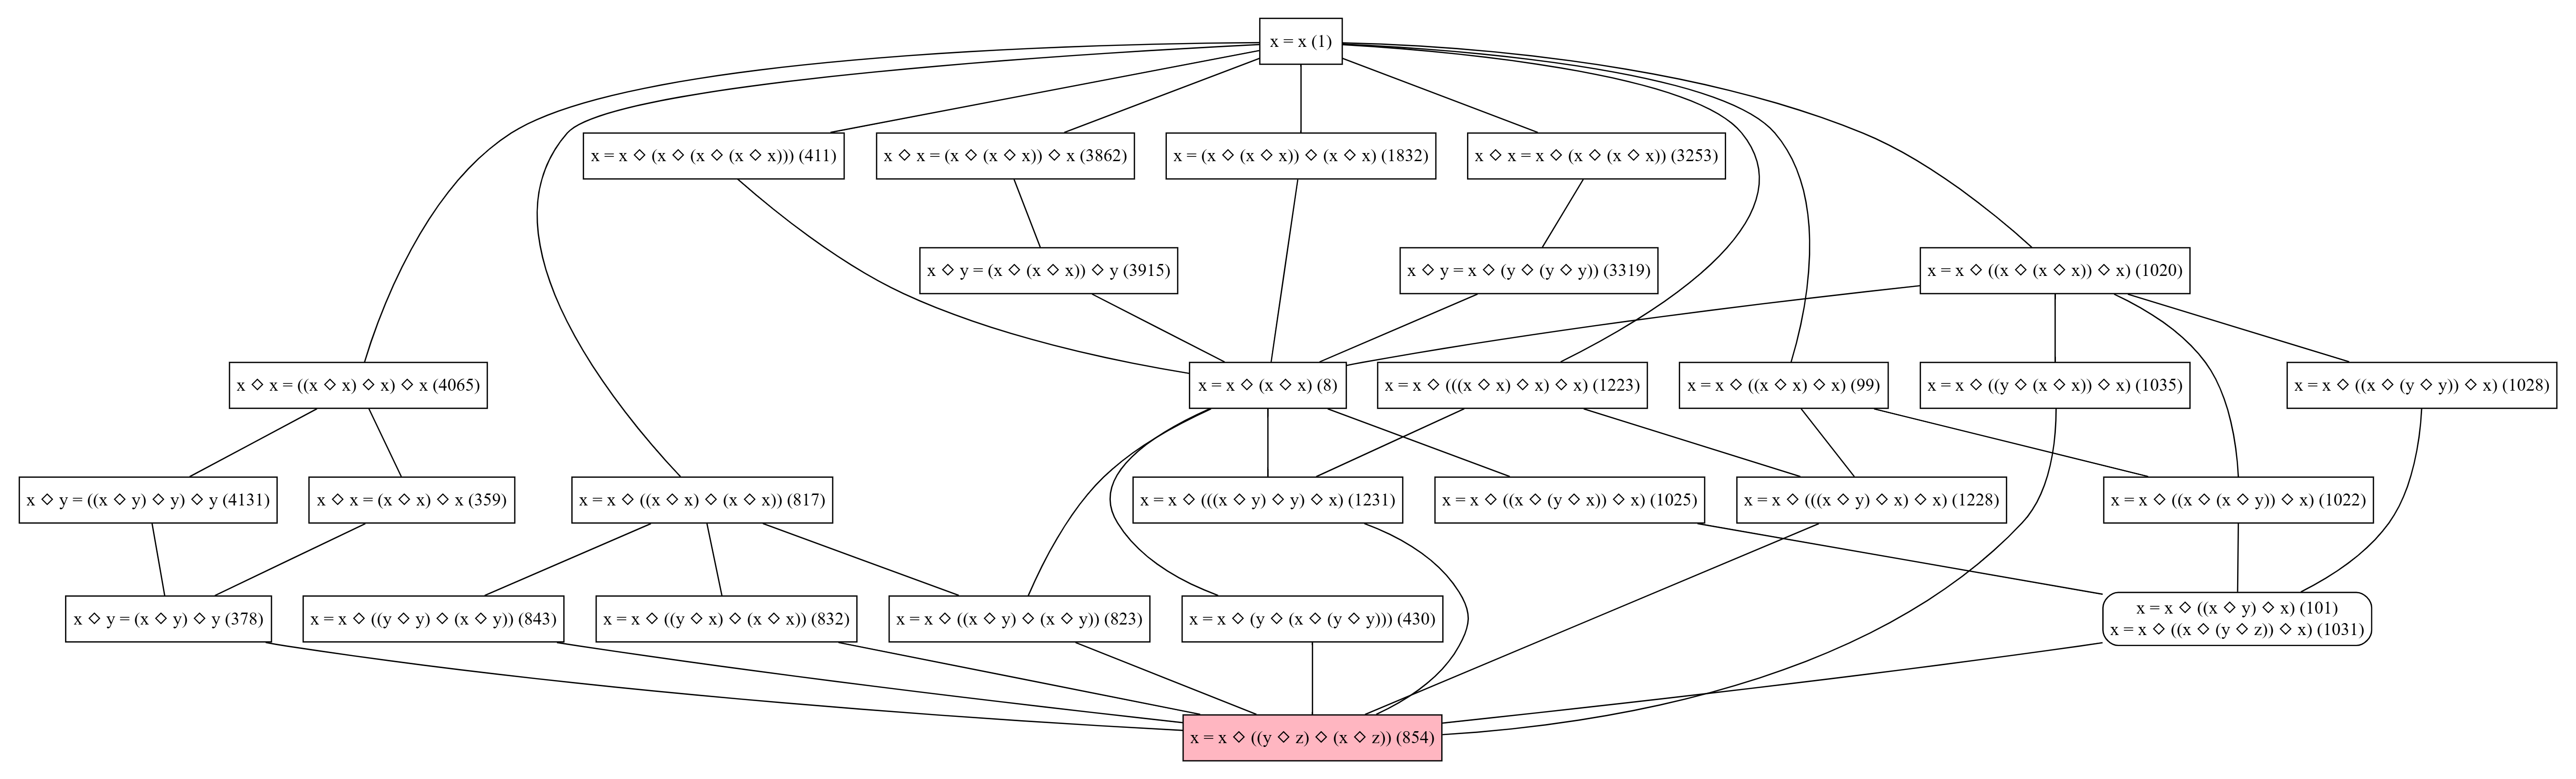
\includegraphics[width=0.85\textwidth]{854.png}
\caption{A Hasse diagram of all the equational laws implied by \eqref{eq854} (for unrestricted magmas).  An edge in this diagram indicates that the lower equation implies the higher one. Rounded rectangles indicate groups of equivalent laws.  This graph was produced by the visualization tool \emph{Graphiti}, which was developed for this project.}
\label{fig:854}
\end{figure}

\begin{figure}
    \centering
    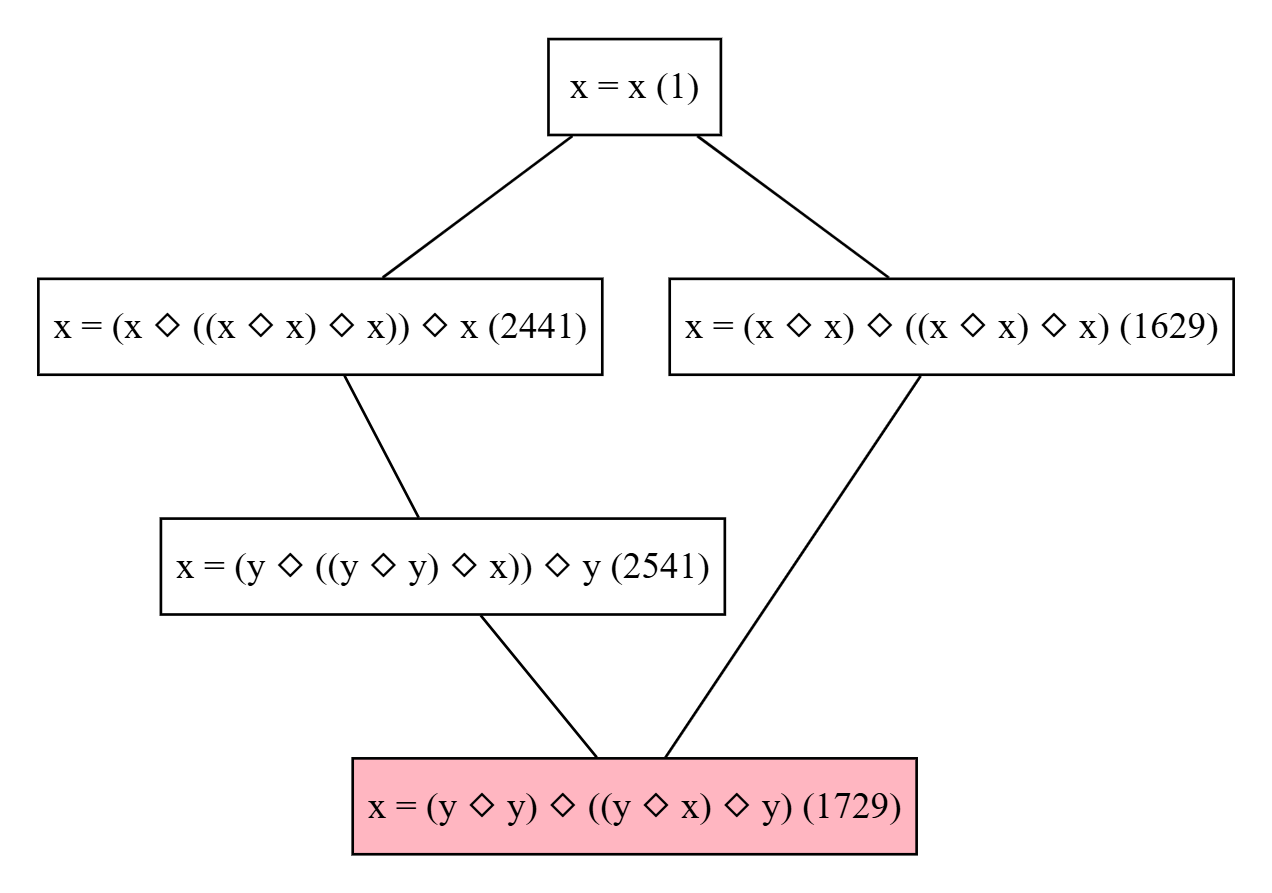
\includegraphics[width=0.4\textwidth]{ramanujan-infinite.png}
    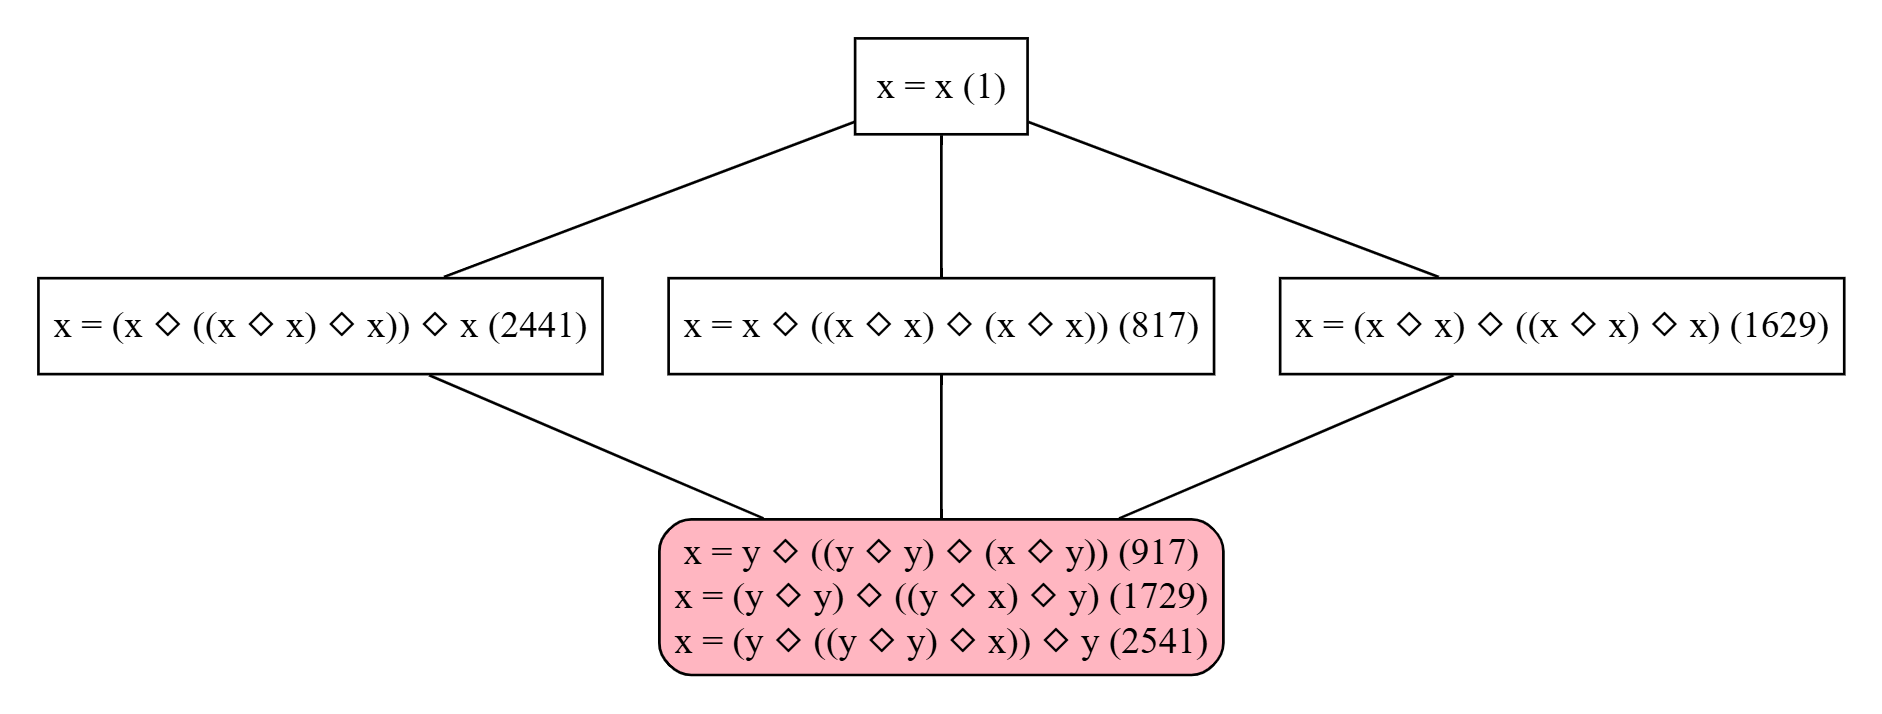
\includegraphics[width=0.4\textwidth]{ramanujan-finite.png}
    \caption{A Hasse diagram of all the equational laws implied by \eqref{eq1729}, both for unrestricted magmas (left) and finite magmas (right). Note the slightly larger number of implications in the latter.}
    \label{fig:1729}
\end{figure}

\begin{figure}
    \centering
    \resizebox{\textwidth}{!}{%
      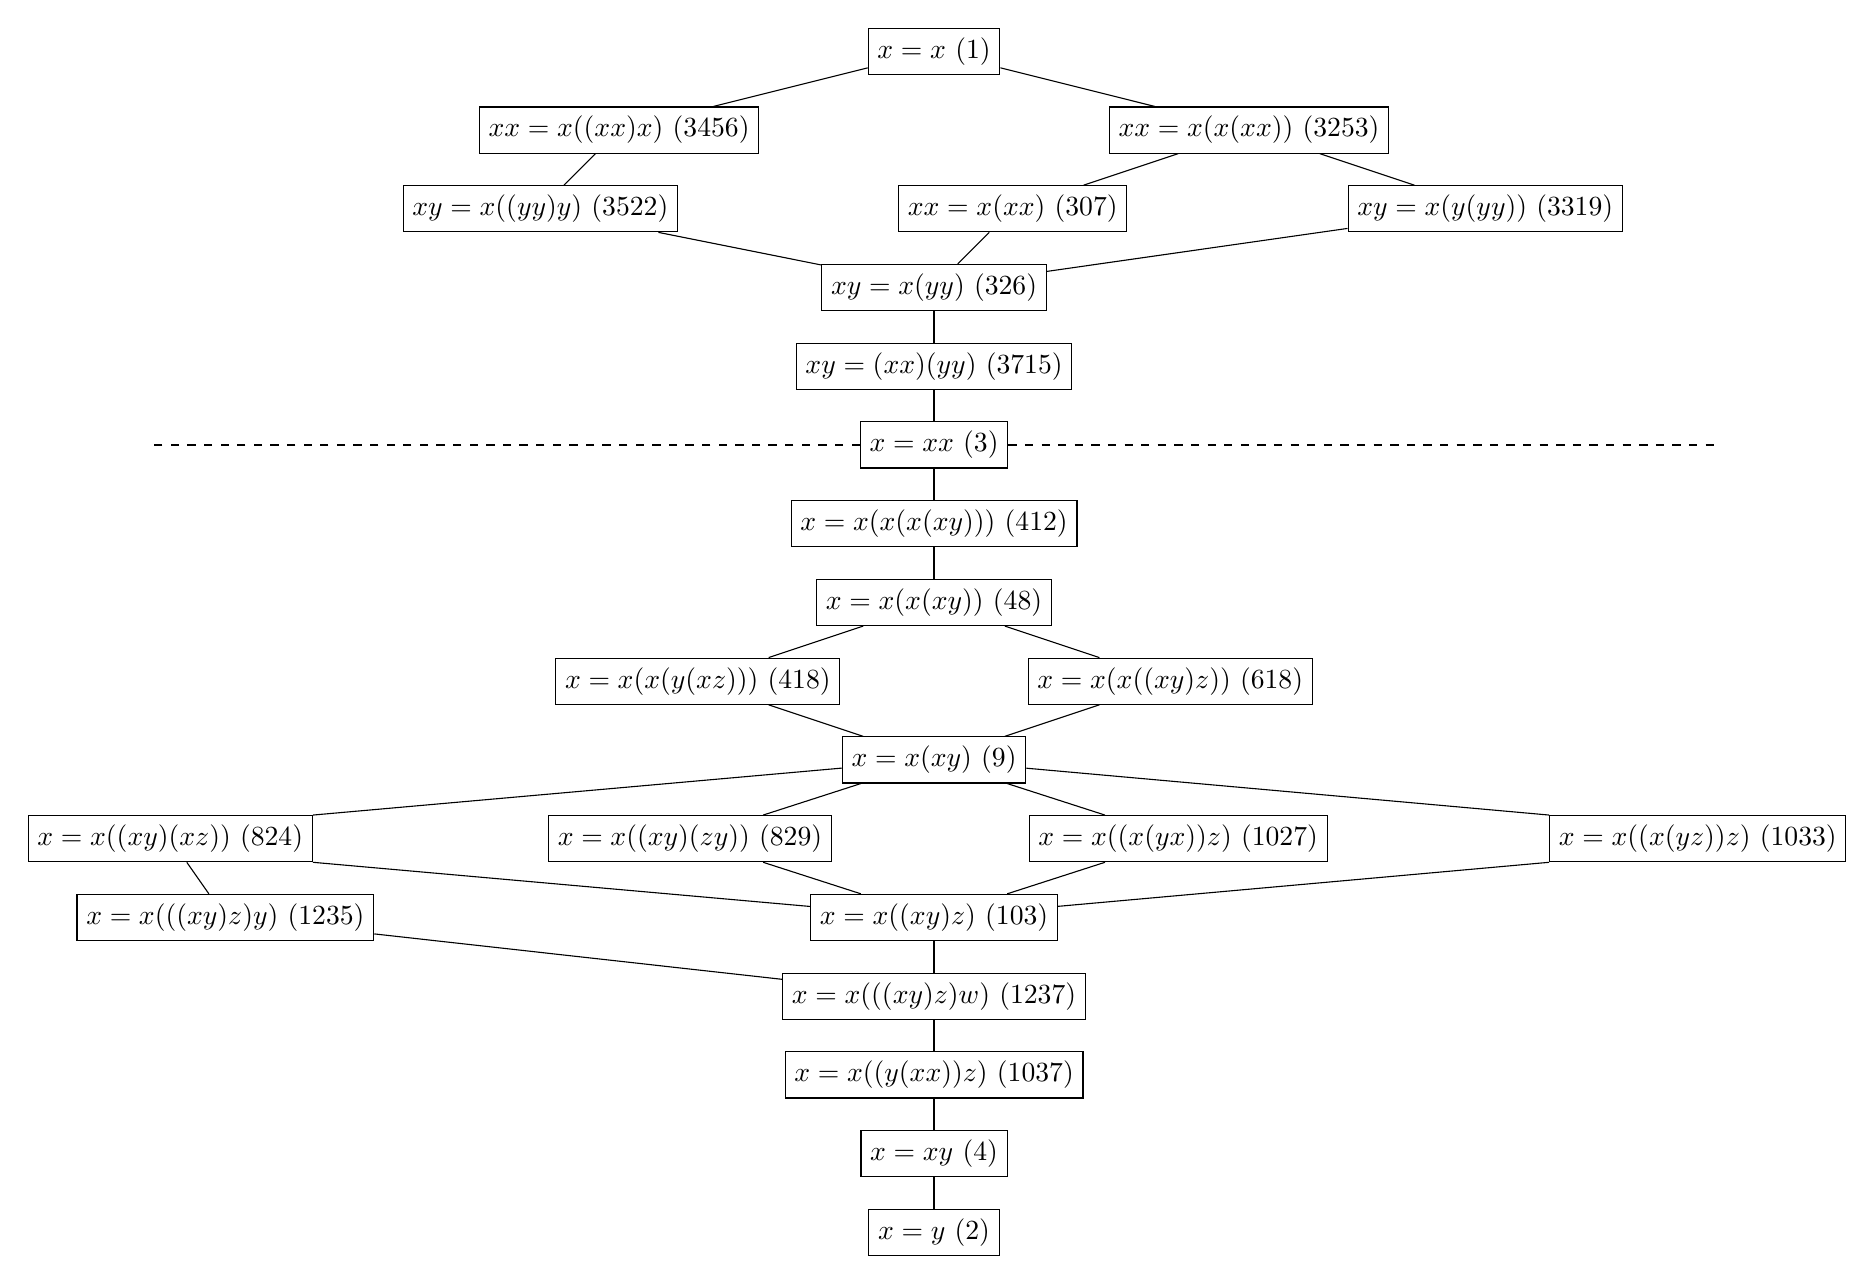
\begin{tikzpicture}
        \node(1)[draw] at (0,15) {$x = x$ (1)};
        \node(3253)[draw] at (4,14) {$x \op x = x \op (x \op (x \op x))$ (3253)};
        \node(3456)[draw] at (-4,14) {$x \op x = x \op ((x \op x) \op x)$ (3456)};
        \node(3319)[draw] at (7,13) {$x \op y = x \op (y \op (y \op y))$ (3319)};
        \node(307)[draw] at (1,13) {$x \op x = x \op (x \op x)$ (307)};
        \node(3522)[draw] at (-5,13) {$x \op y = x \op ((y \op y) \op y)$ (3522)};
        \node(326)[draw] at (0,12) {$x \op y = x \op (y \op y)$ (326)};
        \node(3715)[draw] at (0,11) {$x \op y = (x \op x) \op (y \op y)$ (3715)};
        \node(3)[draw] at (0,10) {$x = x \op x$ (3)};
        \draw[dashed](3)--(-10,10);
        \draw[dashed](3)--(10,10);
        \node(412)[draw] at (0,9) {$x = x \op (x \op (x \op (x \op y)))$ (412)};
        \node(48)[draw] at (0,8) {$x = x \op (x \op (x \op y))$ (48)};
        \node(618)[draw] at (3,7) {$x = x \op (x \op ((x \op y) \op z))$ (618)};
        \node(418)[draw] at (-3,7) {$x = x \op (x \op (y \op (x \op z)))$ (418)};
        \node(9)[draw] at (0,6) {$x = x \op (x \op y)$ (9)};
        \node(824)[draw] at (-9.7,5) {$x = x \op ((x \op y) \op (x \op z))$ (824)};
        \node(829)[draw] at (-3.1,5) {$x = x \op ((x \op y) \op (z \op y))$ (829)};
        \node(1027)[draw] at (3.1,5) {$x = x \op ((x \op (y \op x)) \op z)$ (1027)};
        \node(1033)[draw] at (9.7,5) {$x = x \op ((x \op (y \op z)) \op z)$ (1033)};
        \node(103)[draw] at (0,4) {$x = x \op ((x \op y) \op z)$ (103)};
        \node(1235)[draw] at (-9,4) {$x = x \op (((x \op y) \op z) \op y)$ (1235)};
        \node(1237)[draw] at (0,3) {$x = x \op (((x \op y) \op z) \op w)$ (1237)};
        \node(1037)[draw] at (0,2) {$x = x \op ((y \op (x \op x)) \op z)$ (1037)};
        \node(4)[draw] at (0,1) {$x = x \op y$ (4)};
        \node(2)[draw] at (0,0) {$x = y$ (2)};
        \draw(2)--(4);
        \draw(4)--(1037);
        \draw(1037)--(1237);
        \draw(1237)--(1235);
        \draw(1235)--(824);
        \draw(1237)--(103);
        \draw(103)--(1027);
        \draw(103)--(1033.south west);
        \draw(103)--(824.south east);
        \draw(103)--(829);
        \draw(1027)--(9);
        \draw(1033.north west)--(9);
        \draw(829)--(9);
        \draw(824.north east)--(9);
        \draw(9)--(418);
        \draw(9)--(618);
        \draw(418)--(48);
        \draw(618)--(48);
        \draw(48)--(412);
        \draw(412)--(3);
        \draw(3)--(3715);
        \draw(3715)--(326);
        \draw(326)--(3522);
        \draw(3522)--(3456);
        \draw(3456)--(1);
        \draw(326)--(307);
        \draw(307)--(3253);
        \draw(3253)--(1);
        \draw(326)--(3319);
        \draw(3319)--(3253);
      \end{tikzpicture}%
    }
    \caption{Longest chains of implications (length $15$) between inequivalent laws in the implication graph.  The parts above/below law 3 can be independently dualized. }
    \label{fig:longchain}
\end{figure}

Of the $\num{22033636}$ possible implications $E \vdash E'$, $8178279$ (or $37.12\%$) would end up being true; for an additional set of either $820$ or $822$ pairs $E,E'$, the weaker implication $E \vdashfin E'$ also held. To establish such positive implications $E \vdash E'$ or $E \vdashfin E'$, the main techniques used were as follows:

\begin{itemize}
    \item A very small number of positive implications were established and \textbf{formalized by hand}, mostly through direct rewriting of the laws; but this approach would not scale to the full project.
    \item \textbf{Simple rewriting rules}, for instance based on the observation that any law of the form $\x \formaleq f(\y,\z,\dots)$ was necessarily equivalent to the trivial law \eqref{eq2}, could already reduce the size of potential equivalence classes by a significant fraction. We discuss this method in \Cref{rewrite-sec}.
    \item The preorder axioms for $\vdash$, as well as the ``duality'' symmetry of the preorder with respect to replacing a magma operation $x \op y$ with its opposite $x \op^{\mathrm{op}} y \coloneqq y \op x$, can be used to significantly cut down on the number of implications that need to be proven explicitly; ultimately, only $10657$ ($0.13\%$) of the positive implications needed a direct proof.
    \item To obtain additional implications for finite magmas, heavy reliance was made on the fact that for functions $f \colon M \to M$ on a finite set $M$, surjectivity was equivalent to injectivity.  Some more sophisticated variants of this idea can lead to additional implications; see \Cref{finite-sec}.
    \item \textbf{Automated Theorem Provers} (ATP) could be deployed at extremely fast speeds to establish a complete generating set of positive implications; see \Cref{automated-sec}.
\end{itemize}

More challenging were the $\num{13855357}$ ($62.88\%$) implications that were false, $E \nvdash E'$, and particularly the slightly smaller set of $\num{13854535}$ or $\num{13854537}$ implications that were false even for finite magmas, $E \nvdashfin E'$. Here, the range of techniques needed to refute such implications were quite varied, and may be of independent interest:
\begin{itemize}
        \item \textbf{Syntactic methods}, such as observing a ``matching invariant'' of the law $E$ that was not shared by the law $E'$, could be used to obtain some refutations.  For instance, if both sides of $E$ had the same order, but both sides of $E'$ did not, this could be used to syntactically refute $E \vdash E'$.  Similarly, if the law $E$ was confluent, enjoyed a complete rewriting system, or otherwise permitted some understanding of the free magma associated to that law, one could decide the assertions $E \vdash E'$ for all possible laws $E'$, or at least a significant fraction of such laws.  We discuss these methods, and the extent to which they can be automated, in \Cref{syntactic-sec}.
        \item \textbf{Small finite magmas}, which can be described explicitly by multiplication tables, could be tested by brute force computations to provide a large number of finite counterexamples to implications, or by ATP-assisted methods. See \Cref{finite-sec}.
        \item \textbf{Linear models}, in which the magma operation took the form $x \op y = ax + by$ for some (commuting or noncommuting) coefficients $a,b$, allowed for another large class of counterexamples to implications, which could be automatically scanned for either by brute force or by Grobner basis type calculations; many of these examples could also be made finite. See \Cref{linear-sec}.
        \item \textbf{Translation invariant models}, in which the magma operation took the form $x \op y = x + f(y-x)$ on an additive group, or $x \op y = x f(x^{-1} y)$ on a noncommutative group, reduce matters to analyzing certain functional equations; see \Cref{translation-sec}.
        \item \textbf{Greedy methods}, in which either the multiplication table $(x,y) \mapsto x \op y$ or the function $f$ determining a translation-invariant model are iteratively constructed by a greedy algorithm subject to a well-chosen ruleset, were effective in resolving many implications not easily disposed of by preceding methods. See \Cref{greedy-sec}.
        \item Starting with a simple base magma $\Magma$ obeying both $E$ and $E'$, and either \textbf{enlarging} it to a larger magma $\Magma'$ containing $\Magma$ as a submagma, \textbf{extending} it to a magma $\MagmaN$ with a projection homomorphism $\pi: \MagmaN \to \Magma$, or \emph{modifying the multiplication table} on a small number of values, also proved effective when combined with greedy methods or with a ``\textbf{magma cohomology}'' construction. See \Cref{modify-base}.
        \item To each equation $E$ one can associate a ``\textbf{twisting semigroup}'' $S_E$.  If $S_E$ is larger than $S_{E'}$, then this can often be used to disprove the implication $E \vdash E'$; see \Cref{twisting-sec}.
        \item Some \textbf{ad hoc models} based on existing mathematical objects, such as infinite trees, rings of polynomials, or ``Kisielewicz models'' utilizing the prime factorization of the natural numbers, could also handle some otherwise difficult cases.  In some cases, the magma law induced some relevant and familiar structures, such as a directed graph or a partial order, which also helped guide counterexample constructions. We will not detail these diverse examples here, but refer the reader to the ETP blueprint for more discussion.
        \item \textbf{Automated theorem provers} were helpful in identifying which simplifying axioms could be added to the magma without jeopardizing the ability to refute the desired implication $E \vdash E'$ or $E \vdashfin E'$.
\end{itemize}

While the vast majority of negative implications could be quickly resolved by one of the above techniques, either with human input or in a completely automated fashion, there were perhaps two dozen such negative results that required quite delicate and \emph{sui generis} constructions.  The hardest such implication, $\Eq{1729} \nvdash \Eq{817}$, took several months to establish and then formalize (using a combination of many of the above constructions), with the final proof in \emph{Lean} requiring just over $\num{4000}$ dedicated lines of code from multiple contributors.

In the course of completing the implication graph, some interesting new algebraic structures were discovered.  One such example concerns the magmas obeying \eqref{eq1485}, which we refer to as \emph{weak central groupoids} as they contain the central groupoids (obeying \eqref{eq168}) as a subclass.  In \cite{knuth} it was observed that all finite central groupoids have order equal to a perfect square $n^2$; empirically, we have found that finite weak central groupoids always have order $n^2$ or $2n^2$, although we have no rigorous proof of this claim; they also have a graph-theoretic interpretation analogous to the interpretation of central groupoids as digraphs with the unique path property.  For these and other observations we refer the reader to \href{https://teorth.github.io/equational_theories/blueprint/weak-central-groupoids-chapter.html}{the blueprint of the ETP}.

The objective of using the data from the ETP to establish well-calibrated benchmarks to evaluate ATPs remains an interesting open problem; the participants of this project did not have the required expertise to develop and test such benchmarks to the standards expected in the area.  However, in \Cref{automated-sec} we present a more informal ``field report'' of our experiences using ATPs in the project, in the hope that this will provide some useful guidance to other researchers seeking to incorporate ATPs into their own research.

\begin{figure}
\centering
\begin{tikzpicture}[
    >=Latex,
    node distance=1.1cm,
    every node/.style={draw, rectangle, align=center},
    label/.style={font=\bfseries}
  ]

  %% Column labels
  \node[label] (ghlabel)   at (0,2) {GitHub};
  \node[label] (zuliplabel) at (7,2) {Lean Zulip};

  %% GitHub nodes
  \node (blueprint)   {Blueprint};
  \node (formal)     [below=of blueprint] {Lean formalization};
  \node (viz)        [below=of formal]    {Visualization tools};

  %% Lean Zulip nodes
  \node (hproofs)    [right=of blueprint]       {Human-gen. proofs};
  \node (cproofs)    [right=3cm of formal]         {Computer-gen. proofs};
  \node (hdisc)      [right=of viz]         {Human discussion};

  %% External ATP box
  \node (atp)        [right=of cproofs]         {ATPs, other\\external tools};

  %% Grouping boxes
  % GitHub container
  \node[draw,dotted,inner sep=8pt,fit=(blueprint)(formal)(viz), label=above:GitHub]
    (ghbox) {};
  % Lean Zulip container
  \node[draw,dotted,inner sep=8pt,fit=(hproofs)(cproofs)(hdisc), label=above:Lean Zulip]
    (zulipbox) {};

  %% Arrows
  \draw[human,->] (blueprint)  -- (formal);
  \draw[auto,->] (formal)     -- (viz);
  \draw[human,->] (viz)        -- (hdisc);
  \draw[human,->] (hdisc)      -- (atp);
  \draw[auto,->] (atp)        -- (cproofs);
  \draw[human,->] (cproofs)    -- (hproofs);
  \draw[semi,->] (cproofs)    -- (formal);
  \draw[human,<->] (hproofs)   -- (hdisc);
  \draw[human,->] (hproofs)  -- (blueprint);
  \draw[human,->] (hproofs)  -- (formal);

\end{tikzpicture}
\caption{Some of the main dynamics in which proofs were generated, discussed within the Lean Zulip channel and then formalized in the Github repository.  Boldface arrows indicate human activities, such as proposing an automated attack on outstanding implications, converting a computer-generated proof into a human-readable format, formalizing a human readable proof directly, or first creating a more precise blueprint for other collaborators to work on.  Dashed arrows indicate fully automated processes, while the partly dashed line indicated a semi-automated process requiring human supervision. }
\label{fig:flow}
\end{figure}

\subsection{Further directions}

While the primary objective of the ETP was being completed, some additional related results were generated as spinoffs.  Specifically:
\begin{itemize}
\item In the blueprint on the ETP web site, we report some partial progress on classifying which of the $57882$ distinct laws of order $5$ are equivalent to the singleton law \eqref{eq2}, either with or without the requirement that the magma be finite.
\item In \Cref{higman-neumann} we report on classifying the laws of order $8$ that are equivalent to the Higman-Neumann law \eqref{eq42323216}.
\item In \Cref{ml-sec} we report on preliminary experiments on using machine learning to determine to what extent the implication graph can be predicted by a neural network.
\end{itemize}

\chapter{Selected laws}\label{subgraph-eq}

In this project we study the 4694 laws (up to symmetry and relabeling) of total order at most $4$.

Selected laws of interest are listed below, as well as in \href{https://github.com/teorth/equational_theories/blob/main/equational_theories/Equations.lean}{this file}.

\begin{definition}[Equation 1]\label{eq1}\lean{Equation1}\leanok\uses{magma-def}  Equation 1 is the law $0 \formaleq 0$ (or the equation $x=x$).
\end{definition}

This is the trivial law, satisfied by all magmas. It is self-dual.


\begin{definition}[Equation 2]\label{eq2}\lean{Equation2}\leanok\uses{magma-def}  Equation 2 is the law $0 \formaleq 1$ (or the equation $x=y$).
\end{definition}

This is the singleton law, satisfied only by the empty and singleton magmas.  It is self-dual.

\begin{definition}[Equation 3]\label{eq3}\lean{Equation3}\leanok\uses{magma-def}  Equation 3 is the law $0 \formaleq 0 \op 0$ (or the equation $x = x \op x$).
\end{definition}

This is the idempotence law.  It is self-dual.

\begin{definition}[Equation 4]\label{eq4}\lean{Equation4}\leanok\uses{magma-def}  Equation 4 is the law $0 \formaleq 0 \op 1$ (or the equation $x = x \op y$).
\end{definition}

This is the left absorption law.

\begin{definition}[Equation 5]\label{eq5}\lean{Equation5}\leanok\uses{magma-def}  Equation 5 is the law $0 \formaleq 1 \op 0$ (or the equation $x = y \op x$).
\end{definition}

This is the right absorption law (the dual of Definition \ref{eq4}).

\begin{definition}[Equation 6]\label{eq6}\lean{Equation6}\leanok\uses{magma-def}  Equation 6 is the law $0 \formaleq 1 \op 1$ (or the equation $x = y \op y$).
\end{definition}

This law is equivalent to the singleton law.

\begin{definition}[Equation 7]\label{eq7}\lean{Equation7}\leanok\uses{magma-def}  Equation 7 is the law $0 \formaleq 1 \op 2$ (or the equation $x = y \op z$).
\end{definition}

This law is equivalent to the singleton law.

\begin{definition}[Equation 8]\label{eq8}\lean{Equation8}\leanok\uses{magma-def}  Equation 8 is the law $0 \formaleq 0 \op (0 \op 0)$ (or the equation $x = x \op (x \op x)$).
\end{definition}

\begin{definition}[Equation 14]\label{eq14}\lean{Equation14}\leanok\uses{magma-def}  Equation 14 is the law $0 \formaleq  1 \op (0 \op 1)$ (or the equation $x = y \op (x \op y))$.
\end{definition}

Appears in Problem A1 from Putnam 2001.

\begin{definition}[Equation 16]\label{eq16}\lean{Equation16}\leanok\uses{magma-def}  Equation 16 is the law $0 \formaleq  1 \op (1 \op 0)$ (or the equation $x = y \op (y \op x))$.
\end{definition}

\begin{definition}[Equation 23]\label{eq23}\lean{Equation23}\leanok\uses{magma-def}  Equation 23 is the law $0 \formaleq  (0 \op 0) \op 0$ (or the equation $x = (x \op x) \op x$).
\end{definition}

This is the dual of Definition \ref{eq8}.

\begin{definition}[Equation 29]\label{eq29}\lean{Equation29}\leanok\uses{magma-def}  Equation 29 is the law $0 \formaleq  (1 \op 0) \op 1$ (or the equation $x = (y \op x) \op y)$.
\end{definition}

Appears in Problem A1 from Putnam 2001.  Dual to Definition \ref{eq14}.

\begin{definition}[Equation 38]\label{eq38}\lean{Equation38}\leanok\uses{magma-def}  Equation 38 is the law $0 \op 0  \formaleq  0 \op 1$ (or the equation $x \op x = x \op y$).
\end{definition}

This law asserts that the magma operation is independent of the second argument.

\begin{definition}[Equation 39]\label{eq39}\lean{Equation39}\leanok\uses{magma-def}  Equation 39 is the law $0 \op 0  \formaleq  1 \op 0$ (or the equation $x \op x = y \op x$).
\end{definition}

This law asserts that the magma operation is independent of the first argument (the dual of Definition \ref{eq38}).

\begin{definition}[Equation 40]\label{eq40}\lean{Equation40}\leanok\uses{magma-def}  Equation 40 is the law $0 \op 0  \formaleq  1 \op 1$ (or the equation $x \op x = y \op y$).
\end{definition}

This law asserts that all squares are constant. It is self-dual.

\begin{definition}[Equation 41]\label{eq41}\lean{Equation41}\leanok\uses{magma-def}  Equation 41 is the law $0 \op 0  \formaleq  1 \op 2$ (or the equation $x \op x = y \op z$).
\end{definition}

This law is equivalent to the constant law, Definition \ref{eq46}.

\begin{definition}[Equation 42]\label{eq42}\lean{Equation42}\leanok\uses{magma-def}  Equation 42 is the law $0 \op 1  \formaleq  0 \op 2$ (or the equation $x \op y = x \op z$).
\end{definition}

Equivalent to Definition \ref{eq38}.

\begin{definition}[Equation 43]\label{eq43}\lean{Equation43}\leanok\uses{magma-def}  Equation 43 is the law $0 \op 1  \formaleq  1 \op 0$ (or the equation $x \op y = y \op x$).
\end{definition}

The commutative law. It is self-dual.

\begin{definition}[Equation 45]\label{eq45}\lean{Equation45}\leanok\uses{magma-def}  Equation 45 is the law $0 \op 1  \formaleq  2 \op 1$ (or the equation $x \op y = z \op y$).
\end{definition}

This is the dual of Definition \ref{eq42}.

\begin{definition}[Equation 46]\label{eq46}\lean{Equation46}\leanok\uses{magma-def}  Equation 46 is the law $0 \op 1  \formaleq  2 \op 3$ (or the equation $x \op y = z \op w$).
\end{definition}

The constant law: all products are constant. It is self-dual.

\begin{definition}[Equation 168]\label{eq168}\lean{Equation168}\leanok\uses{magma-def}  Equation 168 is the law $0  \formaleq  (1 \op 0) \op (0 \op 2)$ (or the equation $x = (y \op x) \op (x \op z)$).
\end{definition}

The law of a central groupoid. It is self-dual.

\begin{definition}[Equation 381]\label{eq381}\lean{Equation381}\leanok\uses{magma-def}  Equation 381 is the law $0 \op 1  \formaleq  (0 \op 2) \op 1$ (or the equation $x \op y = (x \op z) \op y$).
\end{definition}

Appears in Putnam 1978, Problem A4, part (b).

\begin{definition}[Equation 387]\label{eq387}\lean{Equation387}\leanok\uses{magma-def}  Equation 387 is the law $0 \op 1  \formaleq  (1 \op 1) \op 0$ (or the equation $x \op y = (y \op y) \op x$).
\end{definition}

Introduced in \href{https://mathoverflow.net/a/450905/766}{MathOverflow}.

\begin{definition}[Equation 953]\label{eq953}\lean{Equation953}\leanok\uses{magma-def}  Equation 953 is the law $0 = 1 \op ((2 \op 0) \op (2 \op 2))$ (or the equation $x = y \op ((z \op x) \op (z \op z))$).
\end{definition}

\begin{definition}[Equation 1571]\label{eq1571}\lean{Equation1571}\leanok\uses{magma-def}  Equation 1571 is the law $0 \formaleq  (1 \op 2) \op (1 \op (0 \op 2))$ (or the equation $x = (y \op z) \op (y \op (x \op z))$).
\end{definition}

Introduced in \cite{mendelsohn-padmanabhan}.

\begin{definition}[Equation 1689]\label{eq1689}\lean{Equation1689}\leanok\uses{magma-def}  Equation 1689 is the law $0 \formaleq  (1 \op 0) \op ((0 \op 2) \op 2)$ (or the equation $x = (y \op x) \op ((x \op z) \op z)$).
\end{definition}

Mentioned in \cite{Kisielewicz2}.

\begin{definition}[Equation 2662]\label{eq2662}\lean{Equation2662}\leanok\uses{magma-def}  Equation 2662 is the law $0 \formaleq  ((0 \op 1) \op (0 \op 1)) \op 0$ (or the equation $x = ((x \op y) \op (x \op y)) \op x$).
\end{definition}

Appears in \cite{mendelsohn-padmanabhan}.

\begin{definition}[Equation 3722]\label{eq3722}\lean{Equation3722}\leanok\uses{magma-def}  Equation 3722 is the law $0 \op 1  \formaleq  (0 \op 1) \op (0 \op 1)$ (or the equation $x \op y = (x \op y) \op (x \op y)$).
\end{definition}

Appears in Putnam 1978, Problem A4, part (a).  It is self-dual.

\begin{definition}[Equation 3744]\label{eq3744}\lean{Equation3744}\leanok\uses{magma-def}  Equation 3744 is the law $0 \op 1  \formaleq  (0 \op 2) \op (3 \op 1)$ (or the equation $x \op y = (x \op z) \op (w \op y)$).
\end{definition}

This law is called a ``bypass operation'' in Putnam 1978, Problem A4. It is self-dual.

\begin{definition}[Equation 4512]\label{eq4512}\lean{Equation4512}\leanok\uses{magma-def}  Equation 4512 is the law $0 \op (1 \op 2)  \formaleq  (0 \op 1) \op 2$ (or the equation $x \op (y \op z) = (x \op y) \op z$).
\end{definition}

The associative law. It is self-dual.

\begin{definition}[Equation 4513]\label{eq4513}\lean{Equation4513}\leanok\uses{magma-def}  Equation 4513 is the law $0 \op (1 \op 2)  \formaleq  (0 \op 1) \op 3$ (or the equation $x \op (y \op z) = (x \op y) \op w$).
\end{definition}

\begin{definition}[Equation 4522]\label{eq4522}\lean{Equation4522}\leanok\uses{magma-def}  Equation 4522 is the law $0 \op (1 \op 2)  \formaleq  (0 \op 3) \op 4$ (or the equation $x \op (y \op z) = (x \op w) \op u$).
\end{definition}

Dual to Definition \ref{eq4579}.

\begin{definition}[Equation 4564]\label{eq4564}\lean{Equation4564}\leanok\uses{magma-def}  Equation 4564 is the law $0 \op (1 \op 2)  \formaleq  (3 \op 1) \op 2$ (or the equation $x \op (y \op z) = (w \op y) \op z$).
\end{definition}

Dual to Definition \ref{eq4513}.

\begin{definition}[Equation 4579]\label{eq4579}\lean{Equation4579}\leanok\uses{magma-def}  Equation 4579 is the law $0 \op (1 \op 2)  \formaleq  (3 \op 4) \op 2$ (or the equation $x \op (y \op z) = (w \op u) \op z$).
\end{definition}

Dual to Definition \ref{eq4522}.

\begin{definition}[Equation 4582]\label{eq4582}\lean{Equation4582}\leanok\uses{magma-def}  Equation 4582 is the law $0 \op (1 \op 2)  \formaleq  (3 \op 4) \op 5$ (or the equation $x \op (y \op z) = (w \op u) \op v$).
\end{definition}

This law asserts that all triple constants (regardless of bracketing) are constant.

We also note some selected laws of order more than $5$.

\begin{definition}[Equation 5105]
  \label{eq5105}\uses{magma-def}
  Equation 5105 is the law $0  \formaleq 1 \circ (1 \circ (1 \circ (0 \circ (2 \circ 1))))$ (or the equation $x = y \circ (y \circ (y \circ (x \circ (z \circ y))))$).
\end{definition}

This law of order $5$ was mentioned in \cite{Kisielewicz2}.

\begin{definition}[Equation 28393]
  \label{eq28393}\uses{magma-def}
  Equation 28393 is the law $0  \formaleq  (((1 \circ 1) \circ 1) \circ 0) \circ (1 \circ 2)$ (or the equation $x = (((y \circ y) \circ y) \circ x) \circ (y \circ z)$).
\end{definition}

This law of order $5$ was introduced by Kisielewicz \cite{Kisielewicz}.

\begin{definition}[Equation 374794]
  \lean{Equation374794}\leanok
  \label{eq374794}\uses{magma-def}
  Equation 374794 is the law $0  \formaleq  (((1 \circ 1) \circ 1) \circ 0) \circ ((1 \circ 1) \circ 2)$ (or the equation $x = (((y \circ y) \circ y) \circ x) \circ ((y \circ y) \circ z)$).
\end{definition}

This law of order $6$ was introduced by Kisielewicz \cite{Kisielewicz}.

The singleton or empty magma obeys all equational laws.  One can ask whether an equational law admits nontrivial finite or infinite models.  An \emph{Austin law} is a law which admits infinite models, but no nontrivial finite models.  Austin \cite{austin} established the first such law, namely the order $9$ law
$$ (((1 \circ 1) \circ 1) \circ 0) \circ (((1 \circ 1) \circ ((1 \circ 1) \circ 1)) \circ 2) \formaleq 0.$$
A shorter Austin law of order $6$ was established in \cite{Kisielewicz}:

\begin{theorem}[Kisielewicz's first Austin law]
  \lean{InfModel.Finite.Equation374794_implies_Equation2,InfModel.Equation374794_not_implies_Equation2}\leanok
  \label{kis-thm}\uses{eq374794,eq2}
  Definition \ref{eq374794} is an Austin law.
\end{theorem}

\begin{proof} \leanok Suppose for contradiction that we have a non-trivial model of Definition \ref{eq374794}. Write $y^2 := y \circ y$ and $y^3 := y^2 \circ y$. For any $y,z$, introduce the functions $f_y: x \mapsto y^3 \circ x$ and $g_{yz}: x \mapsto x \circ (y^2 \circ z)$.  Definition \ref{eq374794} says that $g_{yz}$ is a left-inverse of $f_y$, hence by finiteness these are inverses and $g_{yz}$ is independent of $z$. In particular
$$ f(y^3) = g_{yy}(y^3) = g_{yz}(y^3) = f(y^2 \circ z)$$
and hence $y^2 \circ z$ is independent of $z$.  Thus
$$ f_y(x) = (y^2 \circ y) \circ x = (y^2 \circ y^2) \circ x$$
is independent of $x$.  As $f_y$ is invertible, this forces the magma to be trivial, a contradiction.

To construct an infinite magma, take the positive integers $\Z^+$ with the operation $x \circ y$ defined as
\begin{itemize}
  \item $2^x$ if $y=x$;
  \item $3^y$ if $x = 1 \neq y$;
  \item $\min(j,1)$ if $x=3^j$ and $y \neq x$; and
  \item $1$ otherwise.
\end{itemize}
Then $y^2 = 2^y$, $y^3 = 1$, and $y^2 \circ z$ a power of two for all $y, z$, and $(1 \circ x) \circ w = x$ for all $x$ whenever $w$ is a power of two, so Definition \ref{eq374794} is satisfied.
\end{proof}

An even shorter law (order $5$) was obtained by the same author in a followup paper \cite{Kisielewicz2}:

\begin{theorem}[Kisielewicz theoremII]\label{kis-thm2}\uses{eq2} Definition \ref{eq28393} is an Austin law.
\end{theorem}

\begin{proof} Using the $y^2$ and $y^3$ notation as before, the law reads
\begin{equation}\label{kis2-law}
   x = (y^3 \circ x) \circ (y \circ z).
  \end{equation}
In particular, for any $y$, the map $T_y \colon x \mapsto y^3 \circ x$ is injective, hence bijective in a finite model $G$.  In particular we can find a function $f : G \to G$ such that $T_y f(y) = y^3$ for all $y$  Applying \eqref{kis2-law} with $x = f(y)$, we conclude
$$ T_y(y \circ z) = y^3 \circ (y \circ z) = f(y) $$
and thus $y \circ z$ is independent of $z$ by injectivity of $T_y$.  Thus, the left-hand side of \eqref{kis2-law} does not depend on $x$, and so the model is trivial.  This shows there are no non-trivial finite models.

To establish an infinite model, use $\N$ with $x \circ y$ defined by requiring
$$ y \circ y = 2^y; \quad 2^y \circ y = 3^y$$
and
$$ 3^y \circ x = 3^y 5^x$$
for $x \neq 3^y$, and
$$ (3^y 5^x) \circ z = x$$
for $z \neq 3^y 5^x$.  Finally set
$$ 2^{3^y} \circ z = 3^y$$
for $z \neq 3^y, 2^{3^y}$.  All other assignments of $\circ$ may be made arbitrarily. It is then a routine matter to establish \eqref{kis2-law}.
\end{proof}

In that paper a computer search was also used to show that no law of order four or less is an Austin law.

An open question is whether Definition \ref{eq5105} is an Austin law.  We have the following partial result from \cite{Kisielewicz2}:

\begin{theorem}[Equation 5105 has no non-trivial finite models]\lean{InfModel.Finite.Equation5105_implies_Equation2}\leanok\label{5105-nontrivial}\uses{eq5105} Definition \ref{eq5105} has no non-trivial finite models.
\end{theorem}

\begin{proof} \leanok From Definition \ref{eq5105} we see that the map $w \mapsto y \circ w$ is onto, hence injective in a finite model.  Using this injectivity four times in Definition \ref{eq5105}, we see that $z \circ y$ does not depend on $z$, hence the expression
$x \circ (z \circ y)$ does not depend on $x$.  By Definition \ref{eq5105} again, this means that $x$ does not depend on $x$, which is absurd in a non-trivial model.
\end{proof}

\chapter{Infinite models}

In this chapter we consider non-implications which are refuted only on infinite models, as those are
more challenging to prove---they can't be proved by directly giving an operation table and checking
which laws it satisfies.

We note some selected laws of order more than $5$, used for such non-implications.

\begin{definition}[Equation 5105]
  \label{eq5105}\uses{magma-def}\lean{Equation28393}\leanok
  Equation 5105 is the law $0  \formaleq 1 \op (1 \op (1 \op (0 \op (2 \op 1))))$ (or the equation $x = y \op (y \op (y \op (x \op (z \op y))))$).
\end{definition}

This law of order $5$ was mentioned in \cite{Kisielewicz2}.

\begin{definition}[Equation 28393]
  \label{eq28393}\uses{magma-def}\lean{Equation28393}\leanok
  Equation 28393 is the law $0  \formaleq  (((0 \op 0) \op 0) \op 1) \op (0 \op 2)$ (or the equation $x = (((x \op x) \op x) \op y) \op (x \op z)$).
\end{definition}

This law of order $5$ was introduced by Kisielewicz \cite{Kisielewicz}.

\begin{definition}[Equation 374794]
  \lean{Equation374794}\leanok
  \label{eq374794}\uses{magma-def}
  Equation 374794 is the law $0  \formaleq  (((1 \op 1) \op 1) \op 0) \op ((1 \op 1) \op 2)$ (or the equation $x = (((y \op y) \op y) \op x) \op ((y \op y) \op z)$).
\end{definition}

This law of order $6$ was introduced by Kisielewicz \cite{Kisielewicz}.

The singleton or empty magma obeys all equational laws.  One can ask whether an equational law admits nontrivial finite or infinite models.  An \emph{Austin law} is a law which admits infinite models, but no nontrivial finite models.  Austin \cite{austin} established the first such law, namely the order $9$ law
$$ (((1 \op 1) \op 1) \op 0) \op (((1 \op 1) \op ((1 \op 1) \op 1)) \op 2) \formaleq 0.$$
A shorter Austin law of order $6$ was established in \cite{Kisielewicz}:

\begin{theorem}[Kisielewicz's first Austin law]
  \lean{InfModel.Finite.Equation374794_implies_Equation2,InfModel.Equation374794_not_implies_Equation2}\leanok
  \label{kis-thm}\uses{eq374794,eq2}
  Definition \ref{eq374794} is an Austin law.
\end{theorem}

\begin{proof} \leanok  First we show that every finite model of Definition \ref{eq374794} is trivial.  Write $y^2 := y \op y$ and $y^3 := y^2 \op y$.  For any $y,z$, introduce the functions ${f_y: x \mapsto y^3 \op x}$ and ${g_{yz}: x \mapsto x \op (y^2 \op z)}$.  Definition \ref{eq374794} says that $g_{yz}(f_y(x))=x$, hence by finiteness $g_{yz}=f_y^{-1}$, showing that $g_{yz}$ does not depend on the value of $z$.  Since
$$ f_y(y^2 \op z) = g_{yz}(y^3),$$
it follows that $f_y(y^2 \op z)=f_y(y^3)$ which by injectivity of $f_y$ implies that $z\mapsto y^2 \op z$ is a constant function (with $y$ fixed).  Substituting $y^2$ for $y$ shows that the same is true for $z\mapsto (y^2 \op y^2) \op z$, and since
$$ f_y(z) = (y^2 \op y) \op z = (y^2 \op y^2) \op z$$
we conclude that $f_y$ is also a constant function.  But this function is already known to be injective, thus there do not exist distinct elements in its domain, showing that the model must be trivial.

To construct an infinite model, consider the magma of positive integers $\Z^+$ with the operation $x \op y$ defined by
$$
x \op y = \begin{cases}
2^x, & y=x\\
3^y, & x=1,\ y\not=1\\
\min(j, 1), & x=3^j,\ y \neq x\\
1, & else
\end{cases}.
$$
Then $y \op y = 2^y$ and $(y \op y) \op y = 1$ for all $y$.  Moreover, $(y \op y) \op z$ is a power of two for all $y, z$, and $(1 \op x) \op w = x$ for all $x$ whenever $w$ is a power of two.  It follows that this magma is a model of Definition \ref{eq374794}.
\end{proof}

An even shorter law (order $5$) was obtained by the same author in a follow-up paper \cite{Kisielewicz2}:

\begin{theorem}[Kisielewicz's second Austin law]\label{kis-thm2}\uses{eq2, eq28393} Definition \ref{eq28393} is an Austin law.
\end{theorem}

\begin{proof} Using the $y^2$ and $y^3$ notation as before, the law reads
\begin{equation}\label{kis2-law}
   x = (y^3 \op x) \op (y \op z).
  \end{equation}
In particular, for any $y$, the map $T_y \colon x \mapsto y^3 \op x$ is injective, hence bijective in a finite model $G$.  In particular we can find a function $f : G \to G$ such that $T_y f(y) = y^3$ for all $y$  Applying \eqref{kis2-law} with $x = f(y)$, we conclude
$$ T_y(y \op z) = y^3 \op (y \op z) = f(y) $$
and thus $y \op z$ is independent of $z$ by injectivity of $T_y$.  Thus, the left-hand side of \eqref{kis2-law} does not depend on $x$, and so the model is trivial.  This shows there are no non-trivial finite models.

To establish an infinite model, use $\N$ with $x \op y$ defined by requiring
$$ y \op y = 2^y; \quad 2^y \op y = 3^y$$
and
$$ 3^y \op x = 3^y 5^x$$
for $x \neq 3^y$, and
$$ (3^y 5^x) \op z = x$$
for $z \neq 3^y 5^x$.  Finally set
$$ 2^{3^y} \op z = 3^y$$
for $z \neq 3^y, 2^{3^y}$.  All other assignments of $\op$ may be made arbitrarily. It is then a routine matter to establish \eqref{kis2-law}.
\end{proof}

In that paper a computer search was also used to show that no law of order four or less is an Austin law.

An open question is whether Definition \ref{eq5105} is an Austin law.  We have the following partial result from \cite{Kisielewicz2}:

\begin{theorem}[Equation 5105 has no non-trivial finite models]\lean{InfModel.Finite.Equation5105_implies_Equation2}\leanok\label{5105-nontrivial}\uses{eq5105, models-def} Definition \ref{eq5105} has no non-trivial finite models.
\end{theorem}

\begin{proof} \leanok From Definition \ref{eq5105} we see that the map $w \mapsto y \op w$ is onto, hence injective in a finite model.  Using this injectivity four times in Definition \ref{eq5105}, we see that $z \op y$ does not depend on $z$, hence the expression
$x \op (z \op y)$ does not depend on $x$.  By Definition \ref{eq5105} again, this means that $x$ does not depend on $x$, which is absurd in a non-trivial model.
\end{proof}

We also have such a non-implication involving two laws of order $4$:
\begin{definition}[Equation 3994]
  \label{eq3994}\uses{magma-def}
  Equation 3994 is the law $0 \op 1 \formaleq (2 \op (0 \op 1)) \op 2$ (or the equation $x \op y = (z \op (x \op y)) \op z$).
\end{definition}

\begin{definition}[Equation 3588]
  \label{eq3588}\uses{magma-def}
  Equation 3588 is the law $0 \op 1 \formaleq 2 \op ((0 \op 1) \op 2)$ (or the equation $x \op y = z \op ((x \op y) \op z)$).
\end{definition}

\begin{theorem}[3994 implies 3588 for finite models]\label{finite_imp_3994_3588_thm}\uses{eq3994,eq3588,models-def}
  \lean{InfModel.Finite.Equation3994_implies_Equation3588}\leanok
  All finite magmas which satisfy definition \ref{eq3994} also satisfy definition \ref{eq3588}.
\end{theorem}

\begin{proof}\label{finite_imp_3994_3588} \leanok
  For a finite magma $M$, consider the set $S = \{x \op y | x, y \in M\}$.
  Now $f_z : x \mapsto z \op x$ and $g_z : x \mapsto x \op z$.
  They both map $S$ to $S$, and due to the hypothesis $g_z \op f_z$ is the identity on $S$,
  so because $S$ is finite $f_z$ and $g_z$ must be inverse bijections on it, and therefore
  they commute.
\end{proof}

\begin{theorem}[3994 does not imply 3588 for infinite models]\label{non_imp_3994_3588_thm}\uses{eq3994,eq3588,models-def}
  \lean{InfModel.Equation3994_not_implies_Equation3588}\leanok
  There exists a magma which satisfies \ref{eq3994} and not \ref{eq3588}.
\end{theorem}

\begin{proof} \leanok
  Consider $\mathbb{N}$, with $x \op y$ defined as $x \oplus y$ (bitwise XOR) if $x$ and $y$ are even,
  $y+2$ if only $y$ is even, $x \dot - 2$ if only $x$ is even, and $0$ if both are odd.
  Note that the range of the operation is the set of even naturals.
  Definition \ref{eq3994} is satisfied, because for even $z$ we get $z \oplus (x \op y) \oplus z = x \op y$
  and for odd $z$ we get $(x \op y) + 2 \dot - 2 = x \op y$.
  Setting $x = y = z = 1$, definition \ref{eq3588} isn't satisfied.
\end{proof}

The following result was established in \cite{austin_finite}:

\begin{theorem}[Austin's finite model theorem]\label{austin-two}\uses{models-def} Any law with at most two variables has a non-trivial finite model.
\end{theorem}

\begin{proof}  If neither side of the law is a single variable then the zero law $x \op y = 0$ will work, so one can assume the law takes the form $x = f(x,y)$.  Consider a finite field $F$ with the operation $x \op y := ax+by$ for some coefficients $a,b \in F$.  Then the law becomes a pair of equations $P(a,b)=0$, $Q(a,b)=1$ in the coefficients for some polynomials $P,Q$ with integer coefficients, which one can verify to not divide each other (they have the same degree, and do not have the same set of non-zero monomials).  From Bezout's theorem, this equation has a solution in some field, and hence by the Lefschetz principle it has a solution in a finite field.
\end{proof}

\chapter{General implications}\label{generla-implications-chapter}
We will be interested in seeing which laws imply which other laws, in the sense that magmas obeying the former law automatically obey the latter. We will also be interested in \emph{anti-implications} showing that one law does \emph{not} imply another, by producing examples of magmas that obey the former law but not the latter. Here is a formal definition.

\begin{definition}[Implication]\label{impl}\uses{models-def}
  A law $E$ is said to \emph{imply} another law $E'$ if $\{E\} \models E'$, or equivalently:
  $$ G \models w  \formaleq  w' \implies G \models w''  \formaleq  w''' \hbox{ for all magmas } G$$
  Two laws are said to be \emph{equivalent} if they imply each other.
\end{definition}

\begin{lemma}[Pre-order]\leanok\label{pre-order}\uses{impl}
  If we define $E \leq E'$ if $E$ implies $E'$, then this is a pre-order on the set of laws, and equivalence is an equivalence relation.
\end{lemma}

Note that we view the stronger law as less than or equal to the weaker law. This is because the class of magmas that obey the stronger law is a subset of the class of magmas that obey the weaker law. It is also consistent with the conventions of Lean's Mathlib.

\begin{proof}\leanok
  Trivial.
\end{proof}

Implications between the laws from \Cref{subgraph-eq} are depicted in \Cref{fig:implications}.

\begin{figure}
  \centering
  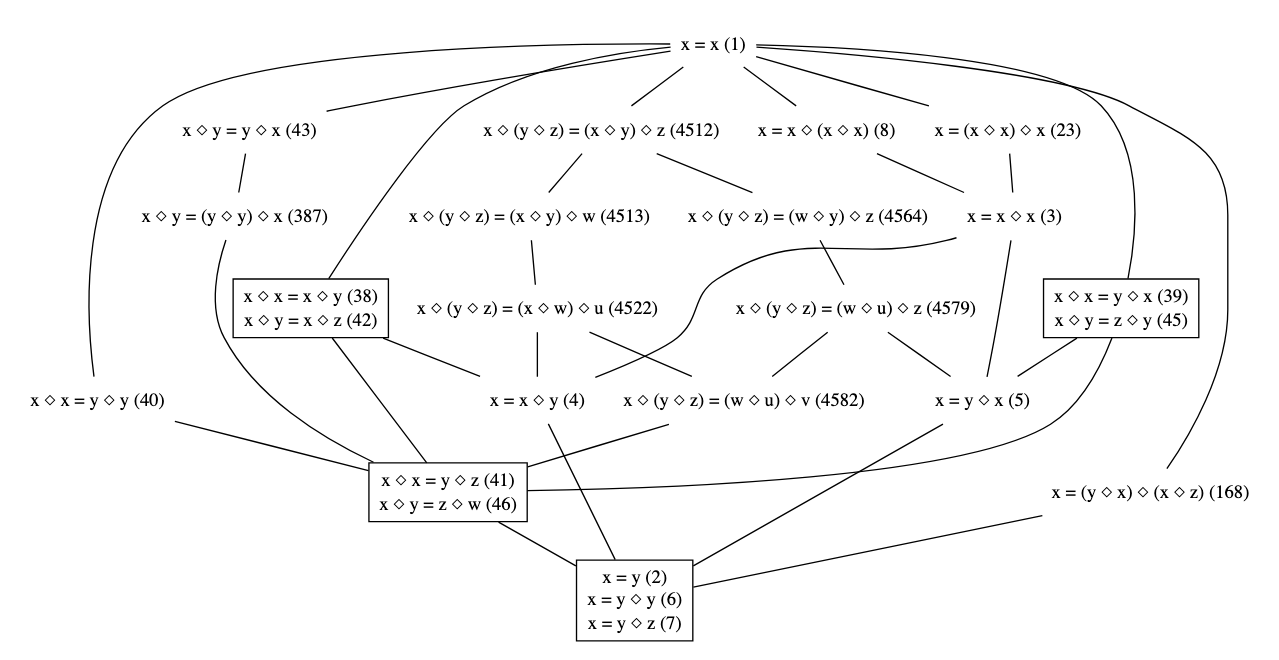
\includegraphics[width=1\linewidth]{../../images/subgraph.png}
  \caption{Implications between the above equations, displayed as a Hasse diagram.}
  \label{fig:implications}
\end{figure}

\begin{lemma}[Maximal element]\label{maximal}\uses{pre-order}\lean{Law.MagmaLaw.Equation1_maximal}\leanok
  The law $0  \formaleq  0$ is the maximal element in this pre-order.
\end{lemma}

\begin{proof}
  Trivial.
\end{proof}

\begin{lemma}[Minimal element]\label{minimal}\uses{pre-order}\lean{Law.MagmaLaw.Equation2_minimal}\leanok
  The law $0  \formaleq  1$ is the minimal element in this pre-order.
\end{lemma}

\begin{proof}
  Trivial.
\end{proof}

Every magma $G$ has a \emph{reversal} $G^{\mathrm{op}}$, formed by by replacing the magma operation $\op$ with its opposite $\op^{\mathrm{op}}:(x,y) \mapsto y \op x$. There is a natural isomorphism between these magmas, which induces an involution $w \mapsto w^{\mathrm{op}}$ on words $w \in M_X$. Every law $w  \formaleq  w'$ then has a \emph{dual} $w^{\mathrm{op}}  \formaleq  (w')^{\mathrm{op}}$.

For instance, the dual of the law $0 \op 1 = 0 \op 2$ is $1 \op 0 = 2 \op 0$, which after relabeling is $0 \op 1 = 2 \op 1$. A list of equations and their duals can be found \href{https://github.com/teorth/equational_theories/blob/main/data/dual_equations.md}{here}. Of the 4694 equations under consideration, 84 are self-dual, leaving 2305 pairs of dual equations.

The pre-ordering on laws has a duality symmetry:

\begin{lemma}[Duality of laws]\lean{Law.MagmaLaw.implies_iff_op}\leanok\label{duality}\uses{pre-order}
  The law $w  \formaleq  w'$ implies $w''  \formaleq  w'''$, if and only if $w^{\mathrm{op}}  \formaleq  (w')^{\mathrm{op}}$ implies $w''^{\mathrm{op}}  \formaleq  (w''')^{\mathrm{op}}$.
\end{lemma}

\begin{proof}
  This follows from the fact that a magma $G$ satisfies a law $w  \formaleq  w'$ if and only if $G^{\mathrm{op}}$ satisfies $w^{\mathrm{op}}  \formaleq  (w')^{\mathrm{op}}$.
\end{proof}

Some equational laws can be ``diagonalized'':

\begin{theorem}[Diagonalization]\label{diag}
  An equational law of the form
  \begin{equation}\label{prediag}
    F(x_1,\dots,x_n) = G(y_1,\dots,y_m),
  \end{equation}
  where $x_1,\dots,x_n$ and $y_1,\dots,y_m$ are distinct elements of the alphabet, implies the diagonalized law
  $$ F(x_1,\dots,x_n) = F(x'_1,\dots,x'_n).$$
  where $x'_1,\dots,x'_n$ are distinct from $x_1,\dots,x_n$
  In particular, if $G(y_1,\dots,y_m)$ can be viewed as a specialization of $F(x'_1,\dots,x'_n)$, then these two laws are equivalent.
\end{theorem}

\begin{proof}
  From two applications of \Cref{prediag} one has
  $$ F(x_1,\dots,x_n) = G(y_1,\dots,y_m)$$
  and
  $$ F(x'_1,\dots,x'_n) = G(y_1,\dots,y_m)$$
  whence the claim.
\end{proof}

Thus for instance, \Cref{eq7} is equivalent to \Cref{eq2}.

\begin{theorem}[Laws implied by the constant law]\label{constant-impl}\uses{impl,eq46}
  If $w, w'$ each have order at least one, then the law $w \formaleq w'$ is implied by the constant law (\Cref{eq46}). If exactly one of $w, w'$ has order zero, and the law $w \formaleq w'$ is not implied by the constant law.
\end{theorem}

\begin{proof}
  Routine.
\end{proof}

\begin{theorem}[Criterion for implication]\label{variable-impl}\uses{impl}\lean{Law.MagmaLaw.SameCount.derive}\leanok
  If $w \formaleq w'$ is such that every variable appears the same number of times in both $w$ and $w'$, and $w \formaleq w'$ implies another law $w'' \formaleq w'''$, then every variable appears the same number of times in both $w''$ and $w'''$.
\end{theorem}

\begin{proof}
  Consider the magma $\mathrm{MS}$ of multisets over an arbitrary set $A$ (which can be seen as finitely supported maps $A\rightarrow \N$), with the multiset addition law $+$. By hypothesis, this magma obeys $w \formaleq w'$, and hence $w'' \formaleq w'''$, giving the claim by comparing the orders of the elements of $A$ appearing in $w''$ and $w'''$ in this magma.
\end{proof}

\chapter{Subgraph implications}

Interesting implications between the subgraph equations in Chapter \ref{subgraph-eq}. To reduce clutter, trivial or very easy implications will not be displayed here.

\begin{theorem}[387 implies 43]\label{387_implies_43}\uses{eq387,eq43}\lean{Subgraph.Equation387_implies_Equation43}\leanok  Definition \ref{eq387} implies Definition \ref{eq43}.
\end{theorem}

\begin{proof}\leanok (From \href{https://mathoverflow.net/a/450905/766}{MathOverflow}).
  By Definition \ref{eq387}, one has the law
\begin{equation}\label{387-again}
  (x \circ x) \circ y = y \circ x.
\end{equation}
Specializing to $y=x \circ x$, we conclude
$$(x \circ x) \circ (x \circ x) = (x \circ x) \circ x$$
and hence by another application of \eqref{eq387} we see that $x \circ x$ is idempotent:
\begin{equation}\label{idem}
  (x \circ x) \circ (x \circ x) = x \circ x.
\end{equation}
Now, replacing $x$ by $x \circ x$ in \eqref{387-again} and then using \eqref{idem} we see that
$$ (x \circ x) \circ y = y \circ (x \circ x)$$
so in particular $x \circ x$ commutes with $y \circ y$:
\begin{equation}\label{op-idem} (x \circ x) \circ (y \circ y) = (y \circ y) \circ (x \circ x).
\end{equation}
Also, from two applications of \eqref{387-again} one has
$$(x \circ x) \circ (y \circ y) = (y \circ y) \circ x = x \circ y.$$
Thus \eqref{op-idem} simplifies to $x \circ y = y \circ x$, which is Definition \ref{eq43}.
\end{proof}

\begin{theorem}[29 equivalent to 14]\label{29_equiv_14} \uses{eq29,eq14}\lean{Subgraph.Equation29_implies_Equation14}\leanok  Definition \ref{eq29} is equivalent to Definition \ref{eq14}.
\end{theorem}

This result was posed as Problem A1 from Putnam 2001.

\begin{proof}\leanok\uses{duality} By Lemma \ref{duality} it suffices to show that Definition \ref{eq29} implies Definition \ref{eq14}.  From Definition \ref{eq29} one has
  $$ x = ((x \circ y) \circ x) \circ (x \circ y)$$
  and also
  $$ y = (x \circ y) \circ x$$
  giving $x = y \circ (x \circ y)$, which is Definition \ref{eq14}.
\end{proof}

\begin{theorem}[14 implies 29]\label{14_implies_29} \uses{eq29,eq14}\lean{Subgraph.Equation14_implies_Equation29}\leanok  Definition \ref{eq14} implies Definition \ref{eq29}.
\end{theorem}

This result was posed as Problem A1 from Putnam 2001.

\begin{proof}\leanok
\end{proof}

% abbrev Equation381 (G: Type u) [Magma G] := ∀ x y z : G, x ∘ y = (x ∘ z) ∘ y
% abbrev Equation3744 (G : Type u) [Magma G] := ∀ x y z w : G, x ∘ y = (x ∘ z) ∘ (w ∘ y)

%theorem Equation3744_implies_Equation381 (G : Type*) [Magma G] (h: Equation3744 G) : Equation381 G :=
%fun x y z ↦ Eq.trans
%  (h x y z y) $ Eq.trans
%  (congrArg (fun a ↦ a ∘ (y ∘ y)) (h x z z x))
%  (Eq.symm $ h (x ∘ z) y (x ∘ z) y)
%/-- Putnam 1978, problem A4, part (a) -/

The following result was problem A4 on Putnam 1978.

\begin{theorem}[3744 implies 3722, 381]\label{3744_implies_3722_381}\uses{eq3744, eq3722, eq381} Definition \ref{eq3744} implies Definition \ref{eq3722} and Definition \ref{eq381}.
\end{theorem}

\begin{proof} By hypothesis, one has
$$x \circ y = (x \circ z) \circ (w \circ y)
  $$
for all $x,y,z,w$.  Various specializations of this give
\begin{align}
 x \circ y &= (x \circ z) \circ (y \circ y) \label{381-1} \\
 x \circ z &= (x \circ z) \circ (x \circ z) \label{381-2} \\
(x \circ z) \circ y &= ((x \circ z) \circ (x \circ z)) \circ (y \circ y) \label{381-3}.
\end{align}
The equation \eqref{381-2} gives Definition \ref{eq3722}, while \eqref{381-1}, \eqref{381-2}, \eqref{381-3} gives
$$ x \circ y = (x\circ z) \circ y$$
which is Definition \ref{eq381}.
\end{proof}

\begin{theorem}[1689 is equivalent to 2]\label{1689_equiv_2}\uses{eq1689, eq2} Definition \ref{eq1689} is equivalent to Definition \ref{eq2}.
\end{theorem}


\begin{proof}\leanok  The implication of Definition \ref{eq1689} from Definition \ref{eq2} is trivial.  The converse is a surprisingly long chain of implications; see pages 326--327 of \cite{Kisielewicz2}.

\end{proof}

\chapter{Selected magmas}\label{selected-magmas-chapter}

Each magma can be used to establish anti-implications: if $\Gamma$ is the set of all laws obeyed by a magma $G$, then we have $\neg E \leq E'$ whenever $E \in \Gamma$ and $E' \not \in \Gamma$.  Large numbers of implications can already be obtained from

\begin{itemize}
  \item All magmas of size at most $4$, up to isomorphism (of which \href{https://oeis.org/A001329}{there are $178\,985\,294$});
  \item All commutative magmas of size $5$, up to isomorphism (of which \href{https://oeis.org/A001425}{there are $254\,429\,900$});
  \item Cyclic groups $\Z/N\Z$ with $2 \leq N \leq 12$ and $x \op y = ax^2+bxy+cy^2+dx+ey$ for randomly chosen $a,b,c,d,e$.
  \item There are only \href{https://oeis.org/A057991}{$1411$ quasigroups of size $5$} (up to isomorphism), and Mace4 can generate all of them in under 20 seconds. A shell script to do this is available \href{https://github.com/zaklogician/equational_theories/tree/cancellative_magmas/scripts/cancellative_magmas}{here}. A magma is a quasigroup if, for all $y$, the left/right multiplications $x\mapsto y\op x$ and $x\mapsto x\op y$ are bijective (equivalent to injective in a finite magma).
\end{itemize}

We also note that a systematic (computer-assisted) study of magmas of size $3$ was performed in \cite{berman-burris}, though with current computational resources it was feasible to iterate over all magmas of size up to $4$ by a brute force approach.

Some other magmas have been used to establish counterexamples:
\begin{itemize}
  \item The cyclic group $\Z/6\Z$ with the addition law.
  \item The natural numbers with law $x \op y = x+1$.
  \item The natural numbers with law $x \op y = xy+1$.
  \item The reals with $x \op y = (x+y)/2$.
  \item The natural numbers with $x \op y$ equal to $x$ when $x=y$ and $x+1$ otherwise.
  \item The set of strings with $x \op y$ equal to $y$ when $x=y$ or when $x$ ends with $yyy$, or $xy$ otherwise (see \href{https://leanprover.zulipchat.com/#narrow/stream/458659-Equational/topic/3102.20does.20not.20imply.203176/near/474656031}{this Zulip thread}).
  \item Vector spaces ${\mathbb F}_2^n$ over ${\mathbb F}_2$, which obey \Equaref{1571} (and hence all the subsequent laws mentioned in \Cref{1571_impl}).
  \item Knuth's construction \cite{knuth} of a central groupoid (\Equaref{168}) as follows.  Let $S$ be a (finite) set with a distinguished element $0$, and a binary operation $*$ such that $x*0=0$ and $0*x=x$   for all $x$, and for each $x,y$ there is a unique $z$ with $x*z=y$.  One can then define a central groupoid on $S \times S$ by defining $(a,b) \op (c,d)$ to equal $(b,c)$ if $c,d \neq 0$; $(b,e)$ if $b*e=c$ is non-zero and $d=0$; and $(a*b,0)$ if $c=0$.  One such example in \cite{knuth} is when $S = \{0,1,2\}$ with $1*1=2*1=2$ and $1*2=2*2=1$.
  \item Cancellative magmas of sizes 7 to 9, found by hand-guided search using various solvers.
  \item Two magmas of cardinality $8$ were \href{https://leanprover.zulipchat.com/#narrow/stream/458659-Equational/topic/using.20z3/near/474918100}{constructed by Z3}.
  \item A large number of ad-hoc finite magmas were constructed using the Vampire theorem prover.  In some cases, inputting theoretical information is useful: see \href{https://leanprover.zulipchat.com/#narrow/channel/458659-Equational/topic/Outstanding.20equations.2C.20v1/near/478066872}{this discussion}.
  \item Linear magmas $x\op y = ax+by$ on various fields, such as ${\mathbb F}_p$ for small primes $p$, have also been used to establish counterexamples.  One such choice is $(p,a,b) = (11,1,7)$. See \href{https://leanprover.zulipchat.com/#narrow/stream/458659-Equational/topic/An.20old.20new.20idea}{this discussion}.  For a noncommutative example, see \href{https://leanprover.zulipchat.com/#narrow/channel/458659-Equational/topic/Outstanding.20equations.2C.20v1/near/477928995.2E01}{this discussion}. For a more systematic exploration of the implications that can be obtained by both commutative and noncommutative linear models, see \href{https://leanprover.zulipchat.com/#narrow/channel/458659-Equational/topic/Non-commutative.20linear.20implications}{this discussion}.
  \item A variation of the translation-invariant magma construction which resolved the Asterix / Obelix anti-implication is used to show that \Equaref{1661} does not imply \Equaref{1657}.
\end{itemize}

\chapter{Infinite magma constructions}\label{infinite-magma-constructions-chapter}

The need to construct infinite magmas primarily arises in the context of \emph{Austin laws} and \emph{Austin pairs}.
An Austin law admits infinite models but no nontrivial finite ones, while an Austin pair consists of
laws $P$ and $Q$ such that every finite model obeying the law $P$ also obeys $Q$, but some
infinite magma obeys $P$ without also obeying $Q$. Examples are given in Chapter~\ref{infinite-model-chapter}.

Here we survey techniques for constructing infinite magmas that serve as counterexamples for implications
between laws. Many of the techniques presented trace their origins to the first analysis of the Asterix equation
(\Cref{eq65}), reviewed in Section~\ref{asterix-section}.

\section{Translation-invariant magmas}

A \emph{translation-invariant magma} is a magma whose carrier $G$ is an Abelian group $G = (G,+)$, and whose magma operation takes the form
$$ y \op x = x + f(x-y)$$
for some function $f: G \to G$.  Thus the translations on $G$ become magma isomorphisms.

\begin{example}
  A magma $G$ satisfying the left (\Cref{eq4}) or right (\Cref{eq5}) absorption laws is translation-invariant.
  Equip the carrier $G$ with an Abelian group structure $(G,+,-,0)$ and define $f: G \to G$ as either $f(x) = x$ or $f(x) = -x$.
\end{example}

\begin{example}
  Linear magmas $x\op y = ax+by$ on a field $(\mathbb{F},+,-,\cdot,0,1)$ are translation-invariant if $a + b = 1$,
  since $(\mathbb{F},+,-,0)$ forms an Abelian group, and one can set $f(x) = bx$.
\end{example}

Note that if an example of the latter sort suffices to refute the implication between $P$ and $Q$ then
by the Lefschetz principle one can construct a counterexample where the field $\mathbb{F}$ is finite.
Consequently, $P$ and $Q$ cannot constitute an Austin pair. However, these linear magmas can still serve
as starting points for the \emph{modified translation-invariant} models studied in Section~\ref{infinite-examples-section}.

\section{The Asterix equation}\label{asterix-section}

Over translation-invariant magmas, equational laws simplify to univariate functional equations.

For instance, writing $x = y+h$, we have
$$ y \op x = x + f(h)$$
$$ x \op (y \op x) = x + f(h) + f^2(h)$$
$$ y \op (x \op (y \op x)) = x + f(h) + f^2(h) + f( h + f(h) + f^2(h) )$$
where $f^2 = f \circ f$, so the Asterix equation for such magmas simplifies to the univariant functional equation
\begin{equation}\label{fh}
   f(h) + f^2(h) + f( h + f(h) + f^2(h) ) = 0
\end{equation}
for $h \in G$.

This equation has some degenerate solutions, for instance we can take $f(h) = c$ for any constant $c$ of order $3$ in $G$.  It is challenging to construct more interesting solutions to this equation; however, we can do this if $G=\Z$ by a greedy algorithm.  We need the following technical definition.

\begin{definition}\label{partial-solution}  A \emph{partial solution} $(E_0, E_1, E_2, f)$ to \eqref{fh} consists of nested finite sets
$$ E_0 \subset E_1 \subset E_2 \subset \Z$$ together with a function $f: E_1 \to E_2$ with the following properties:
\begin{itemize}
  \item[(a)] If $h \in E_0$, then $f(h) \in E_1$, so that $f^2(h)$ is well-defined as an element of $E_2$; furthermore, $h + f(h) + f^2(h)$ lies in $E_1$, so that the left-hand side of \eqref{fh} makes sense; and \eqref{fh} holds.
  \item[(b)] The function $f$ is a bijection from $E_1 \backslash E_0$ to $E_2 \backslash E_1$.
\end{itemize}

We partially order the space of partial solutions to \eqref{fh} by writing $(E_0, E_1, E_2, f) \leq (E'_0, E'_1, E'_2, f')$ if the following properties hold:
\begin{itemize}
  \item $E_i \subset E'_i$ for $i=0,1,2$.
  \item $f$ agrees with $f'$ on $E_0$.
\end{itemize}
When this occurs we say that the partial solution $(E'_0, E'_1, E'_2, f')$ \emph{extends} the partial solution $(E_0, E_1, E_2, f)$.

We define the \emph{empty partial solution} $(E_0,E_1,E_2,f)$ by setting $E_0=E_1=E_2$ to be the empty set, and $f$ to be the empty function; it is the minimal element of the above partial order.
\end{definition}


We have the following iterative construction, that lets us add arbitrary elements to the core domain $E_0$:

\begin{lemma}[Enlarging a partial solution]\label{iteration}\uses{partial-solution} Let $(E_0, E_1, E_2, f)$ be a partial solution to \eqref{fh}, and let $h$ be an element of $\Z$ that does not lie in $E_0$.  Then there exists a partial solution $(E'_0, E'_1, E'_2, f')$ to \eqref{fh} that extends $(E_0, E_1, E_2, f)$, such that $h \in E_0'$.
\end{lemma}

\begin{proof}  Because $f$ maps $E_1 \backslash E_0$ bijectively to $E_2 \backslash E_1$, there are three cases:
\begin{itemize}
  \item $h$ is equal to an element $h_0$ of $G \backslash E_2$.
  \item $h$ is equal to an element $h_0$ of $E_1 \backslash E_0$.
  \item $h$ is equal to $h_1 = f(h_0)$ for some $h_0 \in E_1 \backslash E_0$, so that $h_1 \in E_2 \backslash E_1$.
\end{itemize}

We deal with these three cases in turn.

First suppose that $h = h_0\in G \backslash E_2$.  We perform the following construction.

\begin{itemize}
  \item Choose an element $h_1 \in \Z$ that does not lie in $E_2 \cup \{h_0\}$; this is possible because $E_2$ is finite.
  \item Choose an element $h_2 \in \Z$ such that $h_2, h_0+h_1+h_2$, and $-h_1-h_2$ are all distinct from each other and lie outside of $E_2 \cup \{h_0, h_1\}$; this is possible because $E_2$ is finite.
  \item Promote $h_0$ to $E_0$, promote $h_1, h_0+h_1+h_2$ to $E_1$, and promote $h_2, -h_1-h_2$ to $E_2$, creating new sets
  \begin{align*}
    E'_0 &:= E_0 \cup \{h_0\} \\
    E'_1 &:= E_1 \cup \{h_0, h_1, h_0+h_1+h_2\} \\
    E'_2 &:= E_2 \cup \{h_0, h_1, h_0+h_1+h_2, h_2, -h_1-h_2\}.
  \end{align*}
  Clearly we still have nested finite sets $E'_0 \subset E'_1 \subset E'_2$.
  \item Extend $f : E_1 \to E_0$ to a function $f': E'_1 \to E'_0$ by defining
  \begin{align*}
    f'(h_0) &:= h_1 \\
    f'(h_1) &:= h_2 \\
    f'(h_0+h_1+h_2) &:= -h_1-h_2
  \end{align*}
  while keeping $f'(h)=f(h)$ for all $h \in E_1$.
\end{itemize}
It is then a routine matter to verify that $(E'_0,E'_1,E'_2,f')$ is a partial solution to \eqref{fh} extending $(E_0,E_1,E_2,f)$ and that $E'_0$ contains $h_0$, as required.

Now suppose that $h = h_0 \in E_1 \backslash E_0$, then the quantity $h_1 := f(h_0)$ lies in $E_2 \backslash E_1$.  We perform the following variant of the above construction:
\begin{itemize}
\item Choose an element $h_2 \in \Z$ such that $h_2, h_0+h_1+h_2$, and $-h_1-h_2$ are all distinct and lie outside of $E_2$.  This is possible because $E_2$ is finite.
\item Promote $h_0$ to $E_0$, promote $h_1$ and $h_0+h_1+h_2$ to $E_1$, and promote $h_2, -h_1-h_2$ to $E_2$, thus creating new sets
\begin{align*}
  E'_0 &:= E_0 \cup \{h_0\} \\
  E'_1 &:= E_1 \cup \{h_1, h_0+h_1+h_2\} \\
  E'_2 &:= E_2 \cup \{h_0+h_1+h_2, h_2, -h_1-h_2\}.
\end{align*}
Clearly we still have nested finite sets $E'_0 \subset E'_1 \subset E'_2$.
\item Extend $f : E_1 \to E_0$ to a function $f': E'_1 \to E'_0$ by defining
\begin{align*}
  f'(h_1) &:= h_2 \\
  f'(h_0+h_1+h_2) &:= -h_1-h_2
\end{align*}
while keeping $f'(h)=f(h)$ for all $h \in E_1$.
\end{itemize}
It is then a routine matter to verify that $(E'_0,E'_1,E'_2,f')$ is a partial solution to \eqref{fh} extending $(E_0,E_1,E_2,f)$ and that $E'_0$ contains $h_0$, as required.

Finally, suppose that $h = h_1 = f(h_0)$ for some $h_0 \in E_1 \backslash E_0$, so that $h_1 \in E_2 \backslash E_1$.  Then we perform the following algorithm.
\begin{itemize}
  \item Choose an element $h_2 \in \Z$ such that $h_2, h_0+h_1+h_2$, and $-h_1-h_2$ are all distinct and lie outside of $E_2$.  This is possible because $E_2$ is finite.
  \item Choose an element $h_3 \in \Z$ such that $h_3, h_1+h_2+h_3$, and $-h_2-h_3$ are all distinct and lie outside of $E_2 \cup \{h_2, h_0+h_1+h_2,-h_1-h_2\}$.  This is possible because $E_2$ is finite.
  \item Promote $h_0, h_1$ to $E_0$, promote $h_2, h_0+h_1+h_2, h_1+h_2+h_3$ to $E_1$, and promote $h_3, -h_1-h_2,-h_2-h_3$ to $E_2$, creating new sets
\begin{align*}
  E'_0 &:= E_0 \cup \{h_0, h_1 \}\\
  E'_1 &:= E_1 \cup \{h_1, h_2, h_0+h_1+h_2, h_1+h_2+h_3 \}\\
  E'_2 &:= E_2 \cup \{h_2, h_3, h_0+h_1+h_2, h_1+h_2+h_3, -h_1-h_2, -h_2-h_3\}.
\end{align*}
Clearly we still have nested finite sets $E'_0 \subset E'_1 \subset E'_2$.
\item Extend $f : E_1 \to E_0$ to a function $f': E'_1 \to E'_0$ by defining
\begin{align*}
  f'(h_1) &:= h_2 \\
  f'(h_0+h_1+h_2) &:= -h_1-h_2
  f'(h_2) &:= h_3 \\
  f'(h_1+h_2+h_3) &:= -h_2-h_3
\end{align*}
while keeping $f'(h)=f(h)$ for all $h \in E_1$.
\end{itemize}
It is then a routine matter to verify that $(E'_0,E'_1,E'_2,f')$ is a partial solution to \eqref{fh} extending $(E_0,E_1,E_2,f)$ and that $E'_0$ contains $h_0$, as required.
\end{proof}

\begin{corollary} \label{extend}\uses{partial-solution} Every partial solution $(E_0,E_1,E_2,f)$ to \eqref{fh} can be extended to a full solution $\tilde f: \Z \to \Z$.
\end{corollary}

\begin{proof}\uses{iteration}
  If we arbitrarily well-order the integers, and iterate \Cref{iteration} to add the least element of $\Z \backslash E_0$ in this well-ordering to $E_0$, we obtain an increasing sequence $(E^{(n)}_0, E^{(n)}_1, E^{(n)}_2, f^{(n)})$ of partial solutions to \eqref{fh}, where the $E^{(n)}_0$ exhaust $\Z$: $\bigcup_{n=1}^\infty E^{(n)}_0 = \Z$.  Taking limits, we obtain a full solution $\tilde f$.
\end{proof}

\begin{corollary}\label{no-inject}  There exists a solution $f:\Z \to \Z$ to \eqref{fh} such that the map $h \mapsto h + f(h)$ is not injective.
\end{corollary}

\begin{proof}  Select integers $h_0,h_1,h_2,h'_0,h'_1,h'_2$ such that the quantities
  $$ h_0, h_1, h_2, h_0+h_1+h_2, -h_1-h_2, h'_0, h'_1, h'_2, h'_0+h'_1+h'_2, -h'_1-h'_2$$
  are all distinct, but such that
  $$ h_0 + h_1 = h'_0 + h'_1$$
  (there are many assignments of variables that accomplish this).  Then set
\begin{align*}
  E_0 &:= \{h_0, h'_0\}\\
  E_1 &:= E_0 \cup \{ h_1, h'_1, h_0+h_1+h_2, h'_0+h'_1+h'_2\}\\
  E_2 &:= E_2 \cup \{ -h_1-h_2, -h'_1-h'_2\}
\end{align*}
and define $f: E_1 \to E_2$ by the formulae
\begin{align*}
  f(h_0) &:= h_1 \\
  f(h_1) &:= h_2 \\
  f(h_0+h_1+h_2) &:= -h_1-h_2 \\
  f(h'_0) &:= h'_1 \\
  f(h'_1) &:= h'_2 \\
  f(h'_0+h'_1+h'_2) &:= -h'_1-h'_2.
\end{align*}
One can then check that $(E_0, E_1, E_2, f)$ is a partial solution to \eqref{fh}, and by construction $h \mapsto h + f(h)$ is not injective on $E_1$.  Using \Cref{iteration} to extend this partial solution to a full solution, we obtain the claim.
\end{proof}

\begin{corollary}[Asterix does not imply Obelix]\label{asterix-obelix}\uses{eq65,eq1491}  There exists a magma obeying the Asterix law (\Cref{eq65}) with carrier $\Z$ such that the left-multiplication maps $L_y: x \mapsto y \op x$ are not injective for any $y \in \Z$.  In particular, it does not obey the Obelix law (\Cref{eq1491}).
\end{corollary}

\begin{proof}\uses{no-inject} Note that $L_y (y+h) = y + h + f(h)$, so the injectivity of the left-multiplication maps is equivalent to the injectivity of the map $h \mapsto h + f(h)$.  The non-injectivity then follows from \Cref{no-inject}. Note that the Obelix law clearly expresses $x$ as a function of $y$ and $L_y x = y \op x$, forcing injectivity of left-multiplication, so the Obelix law fails.
\end{proof}

On the other hand, for finite magmas the situation is different:

\begin{proposition}[Asterix implies Obelix for finite magmas]\label{asterix-obelix-finite}\uses{eq65,eq1491}  Any finite magma obeying the Asterix law (\Cref{eq65}) also is left-cancellative and obeys the Obelix law (\Cref{eq1491}).
\end{proposition}

\begin{proof}  From \Cref{eq65} we see the map $z \mapsto y \op z$ is surjective, hence injective on a finite magma; thus the magma is left-cancellative.  Replacing $x$ by $y \op x$ in this law, we see that
$$ y \op x = y \op ((y\op x) \op (y \op (y \op x)));$$
using injectivity, we conclude
$$ x = (y\op x) \op (y \op (y \op x))$$
which is \Cref{eq1491}.
\end{proof}

A very similar argument shows that a finite magma that obeys the Obelix law has $z \mapsto y \op z$ injective, hence surjective, and then obeys the Asterix law.


\section{Greedy algorithm constructions}\label{greedy-section}

In Section~\ref{asterix-section} a magma obeying one law and refuting another was obtained by using the
fact that over translation-invariant magmas, equational laws simplify to univariate functional equations,
and solving the resulting equation using a greedy algorithm.

One way to construct infinite magmas obeying specific laws is via a greedy algorithm construction not on a
one-variable functional equation, but on the operation table of the magma itself.

Here, it is best to work with \emph{partially defined magma operations} on some carrier $G$.  These can be interpreted as ternary relations $R(x,y,z)$ in three variables $x,y,z \in G$ which pass the following ``vertical line test'':

\begin{itemize}
  \item[(VLT)] If $R(x,y,z)$ and $R(x,y,z')$ both hold for some $x,y,z,z' \in G$, then $z=z'$.
\end{itemize}

Such an operation is then associated (via a one-to-one correspondence) to a partially defined operation $\op : S \to G$ for some $S \subset G \times G$, with $R(x,y,z)$ holding if and only if $x \op y$ is well-defined (i.e., $(x,y) \in S$) and equal to $z$.  By abuse of notation, we shall also refer to $R$ as a partially defined magma operation.  Genuine magmas then correspond to the special case where $S = G \times G$, that is to say $x \op y$ is well-defined for all $x,y \in G$.

Given a word $w(x_1,\dots,x_n)$ in variables $x_1,\dots,x_n$ (so $w$ is an element of the free magma on $n$ generators), we can say that $w(x_1,\dots,x_n)$ is \emph{well-defined} with respect to a partially defined magma operation $R$ if it can be fully evaluated using $R$.  For instance, the word $(x \op y) \op z$ is well-defined if there exists $w,u \in G$ such that $R(x,y,w)$ and $R(w,z,u)$ both hold, in which case $(x \op y) \op z$ evaluates to $u$.  Note from the axiom (VLT) that this evaluation is unique, if it exists.  Of course, in a genuine magma, all expressions are well-defined.  We say that an expression $w(x_1,\dots,x_n)$ is \emph{almost well-defined} if all strict subexpressions of $w$ are well-defined.  For instance, $(x \op y) \op z$ is almost well-defined if there exists $w \in G$ such that $R(x,y,w)$ holds.

An equational law $w_1 \formaleq w_2$ involving some variables $x_1,\dots,x_n$ is said to be \emph{locally obeyed} by $R$ if,  whenever $w_1(x_1,\dots,x_n)$, $w_2(x_1,\dots,x_n)$ are almost well-defined, and one of the two expressions is well-defined and evaluates to some output $y$, then the other expression is also well-defined and evaluates to the same output $y$.  For instance, in order for $R$ to locally obey the associative law $(x \op y) \op z = x \op (y \op z)$ (\Cref{eq4512}), we require the following two axioms:
\begin{itemize}
  \item[(4512-1)] If $R(x,y,w)$, $R(w,z,u)$, and $R(y,z,v)$, then $R(x,v,u)$.
  \item[(4512-2)] If $R(y,z,w)$, $R(x,w,u)$, and $R(x,y,v)$, then $R(v,z,u)$.
\end{itemize}
If a law involves a single variable on one side, then we only need one axiom.  For instance, the Asterix law (\Cref{eq65}) is locally obeyed by $R$ if and only if the following axiom holds:
\begin{itemize}
  \item[(65)] If $R(y,x,z)$ and $R(x,z,u)$, then $R(y,u,x)$.
\end{itemize}
Note that if the relation $R$ is associated to a genuine magma operation $\op$, then it locally obeys a law $w_1 \formaleq w_2$ if and only if the magma operation $\op$ obeys the law $w_1 \formaleq w_2$.  For instance, the relation $R$ associated to a globally defined magma operation $\op$ obeys (4512-1) and (4512-2) if and only if the magma is associative.

More generally, one can ask for a ternary relation $R$ to obey some theory $\Gamma$ of universal laws, using the language of one ternary relation $R$, the equality symbol $=$, and possibly some constants (we will shortly introduce three constants $a,b,c$ fo this purpose).

Suppose we have a relation $R$ obeying some theory $\Gamma$ (for instance, (VLT) together with (65)), but which is only finitely supported (there are only finitely many triples $(x,y,z)$ for which $R(x,y,z)$ holds).  Then one can find $a,b \in G$ such that $a \op b$ is currently undefined.  If the carrier $G$ is infinite (e.g., if $G = \N$), one can then find another element $c$ which is \emph{novel}: it is not equal to $a, b$, or any of the $x,y,z$ for which $R(x,y,z)$ hold. In other words, the relation $R$ and the constants $a,b,c$ obey the following additional axioms:
\begin{itemize}
  \item[(novel-1)] $c \neq a$ and $c \neq b$.
  \item[(novel-2)] If $R(x,y,z)$, then $c \neq x$, $c \neq y$, and $c \neq z$.
  \item[(undefined)]  $R(a,b,x)$ does not hold for any $x$.
\end{itemize}

Let us say that a theory $\Gamma$ is \emph{greedily extensible} if, whenever $R$ is a finitely supported ternary relation obeying $\Gamma$, and $a,b,c$ are constants obeying (novel-1), (novel-2), (undefined), then there exists an extension $R'$ of $R$, thus
\begin{itemize}
  \item[(extend)] $R(x,y,z) \implies R'(x,y,z)$ for all $x,y,z$,
\end{itemize}
which is also finitely supported and obeys $\Gamma$, and which also obeys the additional axiom
\begin{itemize}
  \item[(define)] $R'(a,b,c)$.
\end{itemize}
Informally, $R'$ is formed from $R$ by ``forcing'' $a \op b = c$ and then adding other axioms as needed. (Indeed, our construction here can be viewed as a simple analogue of the forcing construction in set theory.)

Observe that if a theory $\Gamma$ containing (VLT) is greedily extensible, then any finitely supported ternary relation $R$ obeying $\Gamma$ on a countably infinite carrier $G$ can be extended to a globally defined relation obeying $\Gamma$, by iteratively selecting the first $(a,b)$ (in some fixed enumeration of $G \times G$) for which $a \op b$ is undefined, and then selecting a novel element $c$ to define as $a \op b$, and applying the greedily extensible property, and then taking a direct limit of the countable sequence of relations thus produced.  This gives a flexible way to construct magmas that obey a given theory $\Gamma$, but which violate some other law $w_1 \formaleq w_2$, as the task then reduces to just finding a partial solution $R$ to $\Gamma$ and some constants $x_1,\dots,x_n$ for which the expressions $w_1(x_1,\dots,x_n), w_2(x_1,\dots,x_n)$ are already well-defined, but not equal to each other.

Unfortunately, most theories are not greedily extensible without further modification.  Consider for instance the theory $\Gamma$ consisting of (VLT) and the Asterix law (65).  Given $a,b,c$ and a finitely supported $R$ obeying $\Gamma$ as well as (novel-1), (novel-2), (undefined), we would like to construct a finitely supported  $R'$ obeying $\Gamma$, (extend), (define).  The naive guess would just be to take the minimal construction
$$ R'(x,y,z) \hbox{ iff } R(x,y,z) \hbox{ or } (x,y,z) = (a,b,c).$$
This can work, but there is an obstruction: if $R(w,a,b)$ for some $w$, then (65) forces $R'(w,c,a)$.  So one would have to enlarge the definition of $R'(x,y,z)$, to hold true if one of the following statements holds:
\begin{itemize}
  \item $R(x,y,z)$ holds.
  \item $(x,y,z) = (a,b,c)$.
  \item $(x,y,z) = (w,c,a)$ for some $w$ with $R(w,a,b)$.
\end{itemize}
This works more often, but there is then a second obstruction: if $R(b,a,b)$, then we now have $R'(b,c,a)$, and (65) then forces $R'(a,a,b)$.  So we need to add a fourth item to the above list defining $R'$:
\begin{itemize}
  \item $(x,y,z) = (a,a,b)$, assuming $R(b,a,b)$ holds.
\end{itemize}
But now if we had $R(a,a,z)$ for some $z \neq b$, this would then create a violation of (VLT).  To fix this, we need to extend $\Gamma$ by adding an additional axiom:
\begin{itemize}
  \item (65') If $R(y,x,y)$, then $R(x,x,y)$.
\end{itemize}
With this modification to $\Gamma$, if we run the above analysis, we now see that if $R(b,a,b)$ hold (so that $R(a,a,b)$ also holds), then (65) will force $R'(a,c,a)$, $R'(b,c,a)$, and $R'(c,c,a)$.  So now the modified definition of $R'$ is that $R'(x,y,z)$ holds if one of the following statements holds:
\begin{itemize}
  \item $R(x,y,z)$ holds.
  \item $(x,y,z) = (a,b,c)$.
  \item $(x,y,z) = (w,c,a)$ for some $w$ with $R(w,a,b)$.
  \item $(x,y,z) = (a,c,a)$, $(b,c,a)$, or $(c,c,a)$, assuming $R(b,a,b)$ holds.
\end{itemize}
One can then finally (for instance, with the assistance of a automated theorem prover) verify that if $R$ is finitely supported and obeys $\Gamma = (VLT) + (65) + (65')$ and $a,b,c$ obey (novel-1), (novel-2), (undefined), then the $R'$ defined above is also finitely supported and obeys $\Gamma$, (extend), (define).  This shows that the theory $\Gamma$ is greedily extensible.

Using this, one can for instance find a magma obeying \Cref{eq65} that fails the left-cancellative property
$$ y \op x = y \op x' \implies x=x'$$
or in terms of ternary relations
\begin{equation}\label{left-inject}
   R(y,x,z) \hbox{ and } R(y,x',z) \implies x=x'
\end{equation}
simply by starting with a partial solution, say on the natural numbers in which (e.g.) $R(1,2,0)$, $R(1,3,0)$ are the only situations in which $R$ holds.  One can easily verify that this obeys (VLT) and (65), (65'), but not \eqref{left-inject}, and so any magma constructed by the above greedy construction will not be left-cancellative.  Since the Obelix law \Cref{eq1491} forces left-cancellativity, this gives an alternate proof of \Cref{asterix-obelix}


\section{A survey of examples}\label{infinite-examples-section}

\bf{Translation-invariant models}

The implication between the laws \Cref{eq1648} and \Cref{eq206} can be refuted by a translation-invariant
magma on the integers. Define the function $f: \mathbb{Z} \to \mathbb{Z}$ by
$$f(x) =
\begin{cases}
  -1  & \text{if } x > 0, \\
   0  & \text{if } x = 0, \\
   1  & \text{if } x < 0,
\end{cases}$$
and consider the translation-invariant magma on $\mathbb{Z}$ given by the operation $x \op y = x + f(y-x)$.

The resulting magma satisfies Equation 1648: one can show this by a case analysis on $f(y-x)$. If $f(y-x)=1$ we have $x \op y = x + f(y-x) = x + 1$, so
$$(x \op y) \op ((x \op y) \op y) = (x + 1) \op ((x + 1) \op y) = (x + 1) \op (x + 2) = (x + 1) - 1 = x.$$
Similar computations verify the other two cases.

However, setting $x=0$ and $y=-1$, we get
$$(x \op (x \op y)) \op y = (x \op 1) \op y = (-1) \op y = -1 \neq x$$
so the magma does not obey \Cref{eq206}. We can conclude

\begin{theorem}[1648 does not imply 206]\label{non_imp_1648_206_thm}\uses{eq1648,eq206,models-def}
  \lean{Equation1648_not_implies_Equation206}\leanok
  There exists a magma which satisfies \Cref{eq1648} and not \Cref{eq206}.
\end{theorem}

There are variation of the translation-invariant constructions refuting implications: e.g. in some cases,
similar constructions are carried out starting with a non-Abelian group. Translation-invariant models
are also useful building blocks for the \emph{modified base model} constructions explained below.

\bf{Modified base models}

For some pairs of laws $P$ and $Q$, it is possible to start with an infinite model $(M,\op)$ obeying both $P$ and $Q$,
then modify the operation $\op$ in a limited way, resulting in a model $(M,\op')$ of $P$ that does not obey $Q$.

This works especially well when this \emph{base model} $(M,\op)$ is a translation-invariant magma in which
the function $f$ takes finitely many different values. This is common: e.g. the translation-invariant model
refuting the implication above is of the required sort!

The strategy is to first modify the magma operation in a naive way, by introducing a counterexample to the
consequent $Q$. This generally yields one or more counterexamples to the antecedent $P$, but one can
\emph{trace} the effects of this initial modification and make further adjustments which restore the
antecedent.

A model refuting the implication between the laws \Cref{eq1659} and \Cref{eq4315} can be constructed using
the modified base model technique. Start with the infinite model $(\mathbb{Z},\op)$ of \Cref{eq1659}
$\mathbb{Z}$ given by the following operation:
$$ x\op y = \begin{cases} x+1 & \text{if } x,y \text{ have the same parity} \\ x -1 & \text{otherwise} \end{cases} $$
A case analysis shows that the magma $(\mathbb{Z},\op)$  satisfies both \Cref{eq1659} and \Cref{eq4315}.
We will eventually \emph{modify} it by setting
$$ x \op' y = \begin{cases} 0 & \text{if } x=0,\: x,y \text{ have the same parity} \\  x+1 & \text{if } x\neq 0,\: x,y \text{ have the same parity} \\ x -1 & \text{otherwise} \end{cases} $$
and checking that $(\mathbb{N}, \op' )$ satisfies \Cref{eq1659} but refutes \Cref{eq4315}.

One finds these modifications using the following strategy:

First, choose some element (tuple) of the carrier $M$ that will constitute a counterexample to the
consequent in the modified model. In this specific case, the consequent, \Cref{eq4315}, can be written as
$$ x \op (y \op x) = x \op (y \op z)$$
in equational form, which always holds when $x = z$. So let's choose the tuple $(0,0,1)$
to constitute the required counterexample. Computing $0 \op (0 \op 0) = 0 \op 1 = -1$ and similarly
$0 \op (0 \op 1) = -1$ suggest that we could force this tuple to be a counterexample by defining a new
operation $\op''$ and setting
$0 \op'' 1$ to something other than $-1$. One seemingly has many choices here: should we take
$0 \op'' 1 =0$, $0 \op'' 1 = 1$, $0 \op'' 1 = 2$, or perhaps even $0 \op'' 1 = -1$?

It's easy to rule out some of the possibilities. For instance, setting $0 \op'' 1 = 1$ would
yield $0 \op'' (0 \op'' 0) = 0 \op'' 1 = \op'' (0 \op'' 1)$ again. The simplest possibility which results in
a counterexample to \Cref{eq4315} sets $0 \op'' 1 = 0$ and $x \op'' y = x \op y$ for any $x \neq 0, y \neq 1$.

Unfortunately, the resulting $(M,\op'')$ would not then obey \Cref{eq1659}. For any $z \in M$, one would have
$$ (0 \op'' 1) \op'' ((1 \op'' 1) \op'' z) = 0 \op'' (2 \op'' z)$$
which equals $0 \op'' 1 = 0$ as desired for even $z$, but equals $0 \op'' 3 = -1 \neq 0$ for odd $z$.

However, since $f$ takes finitely many values in the base model, the breakage is tightly controlled:
by considering what happens if $x \neq 0$ and $y \neq 1$, we see that all new counterexamples to \Cref{eq4315}
have this form. The calculation now suggests defining yet another $\op'''$, where setting
$0 \op''' 3 = 0$ would eliminate
this counterexample. But doing that just moves the issue one level higher: one then has
$$ (0 \op''' 3) \op''' ((3 \op''' 3) \op''' z) = 0 \op''' (4 \op''' z)$$ which equals $0 \op''' 3 = 0$ as desired for even $z$, but equals $0 \op''' 5 = -1 \neq 0$ for odd $z$.

Instead, the infinitely many counterexamples arising from the iterated redefinition can be eliminated
all at once by setting:

$x \op' y = \begin{cases} 0 & \text{if } x=0,\: x,y \text{ have the same parity} \\  x+1 & \text{if } x\neq 0,\: x,y \text{ have the same parity} \\ x -1 & \text{otherwise} \end{cases}$

At this point one might as well truncate the model to $\mathbb{N}$ since the result of the $\op'$
operation is nonnegative whenever the operands are nonnegative. This finishes the construction and proves

\begin{theorem}[1659 does not imply 4315]\label{non_imp_1659_4315_thm}\uses{eq1659,eq4315,models-def}
  \lean{Equation1659_facts}\leanok
  There exists a magma which satisfies \Cref{eq1659} and not \Cref{eq4315}.
\end{theorem}

The result of a modified base model construction can be a finite modification (when $\op$ and $\op'$
differ in finitely many inputs) or one in which they differ in infinitely many coefficients. Note that if the base
model $(M,\op)$ was obtained by a greedy construction, and $(M,\op')$ is a finite modification, then the
modified model could also have been obtained using the same greedy construction. It is not surprising that
more difficult refutations using this construction tend to require the latter sort of modification.


\bf{Greedy constructions}

{\bf add a description of the greedy counterexample for 1703,3 here once issue 506 is resolved}


\section{The Dupont equation}\label{dupont-section}

Now we consider the Dupont equation, \Cref{eq63}, which can be treated by a greedy translation invariant construction that is more complicated than the one considered for the Asterix law in \Cref{asterix-section}.

If we adopt a translation-invariant model
$$ x \op y = x + f(y-x)$$
on some abelian group $G$, then with $y = x+h$, we have
$$ x \op y = x + f(h)$$
$$ x \op (x \op y) = x + f^2(h)$$
$$ y \op (x \op (x \op y)) = y + f(f^2(h)-h)$$
and so the Dupont law $x = y \op (x \op (x \op y))$ becomes the functional equation
\begin{equation}\label{dupont-eq}
  f(f^2(h)-h) = -h.
\end{equation}
One way to solve this equation is to have an automorphism $T: G \to G$ that obeys the identity
$$ T^3 - T = -I,$$
then one can just take $f(h) = T(h)$.  For instance, if $G = \Z^3$, one can take the automorphism $T: \Z^3 \to \Z^3$ defined by
$$ T(x,y,z) := (-z,x+z,y).$$

We now extend this greedily to $\Z^3 \times \Z$ as follows.  Define a \emph{partial solution} $(E_1,E_2,f)$ to be a pair $\Z^3 \subset E_1 \subset E_2 \subset \Z^3 \times \Z$, and a function $f: E_2 \to E_1$ obeying the folowing axioms.
\begin{itemize}
  \item[(a)] The set $E_2 \backslash \Z^3$ is finite.
  \item[(b)] For $h \in \Z^3$, $f(h) = Th$; in particular, $f$ is a bijection on $\Z^3$.
  \item[(c)] For $h \in E_1 \backslash \Z^3$, $f(h) \in E_1$.  Also, $-h + f^2(h) \in E_1$ and $f(-h + f^2(h)) = -h$. Note that this (and (b)) implies that $-h \in E_1$, thus $E_1$ is symmetric around the origin.
  \item[(d)] For $h \in E_2 \backslash E_1$, $f(h) \in E_1$.
  \item[(e)] The elements $-h$, $h - f^2(h)$, and $f^2(h) - h$ for $h \in E_2 \backslash E_1$ are all distinct from each other, and all lie outside of $E_2$.  In particular this forces $f^2(h) \neq 0$, hence $f(h) \neq 0$. It also forces $f^2(h) \neq h$, hence $f(h) \neq h$.
\end{itemize}
Thus for instance one can take $(\Z^3,\Z^3,T)$ as a partial solution.  We say that a partial solution $(E'_1, E'_2, f')$ is an \emph{extension} of $(E_1,E_2,f)$ if $E_1 \subset E'_1$, $E'_2 \subset E_2$, and $f'$ agrees with $f$ on $E_2$.

Informally, $E_1$ represents the portion of $\Z^3 \times \Z$ where we have completely resolved the Dupont equation; the set $E_2 \backslash E_1$ represents the portion for which $f$ (and all forward iterates of $f$) have been defined, but the Dupont equation has not yet been verified; and the elements $-h$, $h - f^2(h)$, and $f^2(h) - h$ for $h \in E_2 \backslash E_1$ are the portion where $f$ is not yet defined, but for which one is ready to ``promote'' these elements to $E_2$ or $E_1$ by defining $f$ appropriately.

The key lemmas are then

\begin{lemma}[Promoting to $E_1$]\label{add-E1}  If $(E_1,E_2,f)$ is a partial solution and $h \in E_2 \backslash E_1$, then there exists an extension $(E'_1,E'_2,f')$ of $(E_1,E_2,f)$ such that $h \in E'_1$.
\end{lemma}

\begin{proof} This will be a greedy construction, but we have to introduce a rather large number of additional elements to ensure that certain non-degeneracy conditions are maintained (in particular, the new elements $h'$ introduced have to be such that $f^2(h') - h'$ avoids $E_2$ and hence $\Z^3$, which requires a certain amount of complexity in the construction).

  Let $\tilde E_2$ denote the set $E_2$ together with all the elements of the form $-h'$, $h' - f^2(h')$, and $f^2(h') - h'$ for $h' \in E_2 \backslash E_1$; this is $\Z^3$ with a finite number of additional elements.

Let $a$ be an element of $\Z^3$ such that the quantities
$$ \pm Ta, \pm(Ta + a)$$
are distinct from each other and from
$$0, \pm h, \pm (h - f(h)), \pm (f^2(h)-h);$$
this is possible since $T, T+1$ are invertible.

Next, we pick an $x \in \Z^3 \times \Z$ such that the quantities
$$ \pm x, \pm x + Ta, \pm x - Ta, \pm 2 x + Ta, \pm x + Ta + a, \pm (h + x), \pm (h - f(h) + x), \pm (f^2(h)-h + x + Ta)$$
are all distinct from each other and from $\tilde E_2$; indeed, from the choice of $a$ (and the non-zero nature of $h$, $f(h)$, $h-f(h)$, and $f^2(h)-h$) there are only finitely many $x$ for which a collision can occur between any pair of these expressions.

We now promote $\pm h, \pm x, \pm x + Ta, \pm x - Ta$ to $E_1$, and also promote $h+x$, $h - f^2(h)$, $\pm 2x + Ta$, $\pm x + Ta + a$ to $E_2$.  That is to say, we define
$$ E'_1 := E_1 \cup \{\pm h, \pm x, \pm x + Ta, \pm x - Ta\}$$
and
$$ E'_2 := E_2 \cup \{ -h, \pm x, \pm x + Ta, \pm x - Ta, h + x, h - f^2(h), \pm 2x + Ta \}.$$
We then define an extension $f'$ of $f$ to $E'_2$ by setting
\begin{align*}
 f'(\pm x) &:= a \\
 f'(\pm x + Ta) &:= \pm x \\
 f'(\pm x - Ta) &:= \mp x + Ta \\
 f'(\pm x + Ta + a) &:= \pm x - Ta \\
 f'(\pm 2x + Ta) &:= \pm x + Ta \\
 f'(\pm x + Ta + a) &:= \pm x - Ta \\
 f'(-h) &:= x + Ta \\
 f'(h+x) &:= h \\
 f'(h - f^2(h)) &:= -h.
\end{align*}
It is easy to see that $(E'_1,E'_2,f')$ obeys properties (a), (b), (d).  By construction, we have
$$ f'( (f')^2(h') - h') = -h'$$
for
$$ h' = \pm h, \pm x, \pm x+Ta, \pm x-Ta$$
giving property (c).  By construction, the quantities
$$ -h', h' - f^2(h'), f^2(h') - h'$$
are distinct from each other and lie outside of $\tilde E_2 \cup E'_2$ for
$$ h' = h+x, h - f^2(h), \pm 2x + Ta, \pm x + Ta + a$$
while these quantities are distinct from each other and lie in $\tilde E_2 \backslash E'_2$ for $h' \in E_2 \backslash E'_1$ (note that this forces $h' \neq \pm h$).  This gives property (e).
\end{proof}


\begin{lemma}[Promoting to $E_2$]\label{add-E2}  If $(E_1,E_2,f)$ is a partial solution and $h \in (\Z^3 \times \Z) \backslash E_2$, then there exists an extension $(E'_1,E'_2,f')$ of $(E_1,E_2,f)$ such that $h \in E'_2$.
\end{lemma}

\begin{proof}  Let $\tilde E_2$ denote the set $E_2$ together with all elements of the form
\begin{equation}\label{hp-form}
 -h', h' - f^2(h'), f^2(h') - h'
\end{equation}
for some $h' \in E_2 \backslash E_1$; this is $\Z^3$ with a finite number of elements attached, and is symmetric aroudn the origin.

First suppose that $h$ lies outside of $\tilde E_2$.  Then we can find $a \in \Z^3$ such that the quantities
$$ -h, \pm (h - Ta)$$
are distinct from each other, and lie outside of $\tilde E_2$.  We now promote $h$ to $E_2$, thus setting
$$ E'_1 := E_1$$
and
$$ E'_2 := E_2 \cup \{h\}$$
and define an extension $f'$ of $f$ to $E'_2$ by setting
$$ f'(h) := a.$$
It is then a routine matter to check that $(E'_1,E'_2,f')$ is an extension of $(E_1,E_2,f)$.

Now suppose that $h$ lies in $\tilde E_2$.  Then $h$ is of one of the forms \eqref{hp-form} for some $h' \in E_2 \backslash E_1$.  Suppose it is of the form $-h'$ or $f^2(h') - h'$.  We invoke \Cref{add-E1} to promote $h'$ to $E_1$ by using a suitable extension $(E'_1,E'_2,f')$; and now $h$ will lie in $E'_2$, giving the claim.  If instead $h$ is of the form $h'-f^2(h')$, then this procedure might not place $h$ in $E'_2$; but if it does not, it will be of the form $-h''$ for $h'' = f^2(h')-h' \in E'_2 \backslash E'_1$.  Applying \Cref{add-E1} one more time to now promote $h''$ to $E_1$, we will obtain a larger extension $(E''_1,E''_2,f'')$ with $h \in E''_2$, giving the claim.
\end{proof}

Iterating these lemmas in the usual fashion, we can conclude that any partial solution can be completed to a global model of \Cref{eq63}.

Among other things, this permits one to generate models in which the function $f$ is not injective.  To see this, let $a$ be a non-zero element of $\Z^3$, let $x$ be an element of $\Z^3 \times \Z$ outside of $\Z^3$, and consider the partial solution $(\Z^3, \Z^3 \cup \{x\}, f)$ where $f(h) = Th$ for $h \in \Z^3$ and $f(x) = a$.  One can check that this is a partial solution and is not injective, since $f(x) = f(T^{-1} a)$.  This non-injectivity implies in particular that the model is not left-cancellative, and hence does not obey the law
$$ x = (y \op x) \op ((y \op x) \op y)$$
(equation 1692).

\chapter{Equivalence with the constant and singleton laws}\label{constant-chapter}

\href{https://github.com/teorth/equational_theories/blob/main/equational_theories/Generated/Constant.lean}{85 laws}
have been shown to be equivalent to the constant law (\Equareffull{46}), and
\href{https://github.com/teorth/equational_theories/blob/main/equational_theories/Generated/Singleton.lean}{815 laws}
have been shown to be equivalent to the singleton law (\Equareffull{2}).

These are the laws up to 4 operations that follow from diagonalization of \Equaref{2} and \Equaref{46}.

To formalize these in Lean, a search was run on the list of equations to discover
diagonalizations of these two specific laws: equations of the form $x = R$ where $R$ doesn't include
$x$, and equations of the form $x \circ y = R$ where $R$ doesn't include $x$ or $y$.

The proofs themselves all look alike, and correspond exactly to the two steps described in the proof
of \Cref{diag}. The Lean proofs were generated semi-manually, using search-and-replace starting from
the output of \texttt{grep} that found the diagonalized laws.

In the case of the constant law, \Equareffull{41} wasn't detected using
this method. It was added manually to the file with the existing proof from the sub-graph project.

\chapter{Metatheorems from Invariants}\label{metatheory-chapter}

For the purposes of this chapter, a \emph{theorem} is a (true) statement about particular equations, for example `(387 implies 43)' is a theorem. A \emph{metatheorem} is a general statement about implications; one can usually get many theorems from a single metatheorem. This chapter is all about generating many interesting metatheorems using a \emph{meta-metatheorem}, called the fundamental property of invariants. If all this is making your head spin, don't worry. Look at the sections below for examples of metatheorems you can probably agree are both concrete and interesting. Once you have done that, come back here and we will show you how to prove these and other metatheorems using \emph{invariants}.

\section{Invariants}
Let $E, E_1$, and $E_2$ be equations. If $E \Rightarrow E_1$ and $E_1 \Rightarrow E_2$, then $E \Rightarrow E_2$. Very trivial. Rephrasing this, we see that if $E \Rightarrow E_1$ and $E \nRightarrow E_2$, then $E_1\nRightarrow E_2$.

Extending this idea, suppose we compute the set of all equations which are implied by $E$; we will call this set $\mathcal{Y}(E)$ (we use $\mathcal{Y}$ because this is an example of a \href{https://en.wikipedia.org/wiki/Yoneda_lemma#The_Yoneda_embedding}{Yoneda embedding}). Then $\mathcal{Y}(E)$ is upwards closed, or closed under forward implication: no equation in $\mathcal{Y}(E)$ can imply an equation not in $\mathcal{Y}(E)$. If we know $\mathcal{Y}(E)$ well, this already settles a potentially large number of implications in the negative.

While computing $\mathcal{Y}(E)$ for an arbitrary equation $E$ may seem daunting, for some nice equations we can find \emph{invariants}, which makes the task manageable. An \emph{invariant} for $E$ is some sort of data associated with expressions $w$ so that
\[
\mathcal{Y}(E) = \{w = w' \mid \text{Invariant}(w) = \text{Invariant}(w')\}
\]
If we can find an invariant which is computable for each term $w$, then we can easily describe $\mathcal{Y}(E)$. The fact that $\mathcal{Y}(E)$ is upwards closed is rephrased as follows; this is called \textbf{the fundamental property of invariants}. Remember that an invariant is a function taking expressions and outputting some data.

\begin{metametatheorem}[Fundamental property of invariants]
	Let $I$ be an invariant of $E$. If $w = w'$ implies $w'' = w'''$ and $I(w) = I(w')$ (that is, $E$ implies $w = w'$), then $I(w'') = I(w''')$.
\end{metametatheorem}

More succinctly, for an invariant $I$ of $E$ we must have
\[
(w = w' \Rightarrow w'' = w''') \implies (I(w) = I(w') \Rightarrow I(w'') = I(w''')).
\]
When using this result, we commonly take the contrapositive: if $I(w) = I(w')$ and $I(w'') \neq I(w''')$, then $w=w'$ cannot imply $w'' = w'''$. Note that the conclusion is independent of the equation $E$; all we need to know is that $I$ is an invariant.


%I am stealing the proof environment for a note - this is probably bad practice.
\begin{proof}[Note for category theorists]\leanok
	Let $\Pi$ denote the preorder of magma equations ordered by implication. If $I$ is an invariant then define
	\[
	I(w = w')\coloneqq \begin{cases}
		\texttt{true} & \text{ if }I(w) = I(w')\\
		\texttt{false} & \text{ otherwise}
	\end{cases}.
	\]
	(In programming languages we would say $I(w = w') \coloneqq I(w) == I(w')$). Let $\textbf{Bool} = \{ \texttt{true}, \texttt{false}\}$ be the poset where $\texttt{false} \leq \texttt{true}$. Then $I$ becomes a function $\Pi \to \textbf{Bool}$, and the fundamental property of invariants just says that this function is monotone, i.e. functorial. Thus for every invariant $I$ we obtain a functor $\Pi \to \textbf{Bool}$.

	Question 1: Does every functor $\Pi \to \textbf{Bool}$ come from an invariant?

	Question 2: What can we say about the category of functors $\Pi \to \textbf{Bool}$? Give a nice interpretation of natural transformations between invariants.
\end{proof}

The fundamental property of invariants is not a theorem, nor a metatheorem: it is a meta-metatheorem, in the sense that it will allow us to get a metatheorem for every invariant we find.

\subsubsection*{Example: absorption law}
Let $E$ be the equation $x \op y = x$. Intuitively, we must have
\[
\mathcal{Y}(E) = \{w = w' \mid \text{the leftmost variable is the same for $w$ and $w'$}\}.
\]
We will talk about proving statements like this one (say in Lean) later on; take it as given for now. The invariant is clear: we define $I(w)$ to be the leftmost variable of $w$. Instantiating this invariant in the fundamental property of invariants, we get the following metatheorem.
\begin{metatheorem}
	Let $w = w'$ be an equation such that the leftmost variable of $w$ is the same as the leftmost variable of $w'$. Then $w = w'$ cannot imply an equation that does not have the property from the last sentence.
\end{metatheorem}

\subsubsection*{Example: associativity}
For a more complicated example, let $E$ be the associativity equation $x \op (y \op z) = (x \op y) \op z$. Intuitively, we must have
\[
\mathcal{Y}(E) = \{\text{equations that, when we remove all parentheses, are of the form $w = w$}\}.
\]
There is an invariant lurking behind: it is the (ordered) list of variables appearing in an expression, counting repetitions. More formally, we define $I(w)$ to be the tuple of variables appearing in $w$, listed from left to right, say. Again, from the fundamental property of invariants we get the following.
\begin{metatheorem}
	Let $w = w'$ be an equation such that the variables appearing in $w$, taking into account order and repetitions, are the same ones that appear in $w'$. Then $w = w'$ cannot imply an equation that does not have the property from the last sentence.
\end{metatheorem}

If we were coding a computer program that computes $I(w)$ given $w$, one could take the string of symbols that is $w$, ignore all parentheses, replace all symbols $\op$ by commas, and surround with an appropriate delimiter. (I imagine one could easily do this using \href{https://en.wikipedia.org/wiki/Regular_expression}{regular expressions}.

We can compute other examples, but the invariant can get complicated even for simple equations. Exercise: what is the invariant for commutativity? Answer: To compute $I(w)$ from $w$ replace all parentheses with curly braces and all symbols $\op$ with commas, and interpret the result as nested sets.

\section{Expanding the language}
The method of invariants really shines when we expand our formal language. Right now our language consists of variables, parentheses, the equal sign, and $\op$ (there is also an implicit use of $\forall$ but let's ignore that for now).  Let $\Pi$ denote the preorder of equations (built from the language described) ordered by implication.

We will add the symbol $\wedge$ (`and') to our language. Then we consider a bigger preorder $\Pi' \supseteq \Pi$ which includes equations and also conjunctions of equations. Even if we only care about $\Pi$ it will be apparent that studying invariants in $\Pi'$ gives us useful metatheorems about $\Pi$. Equations and conjunctions of equations are examples of \emph{formulas} (or formulae, according to taste).

If $\varphi$ is a formula, we can define $\mathcal{Y}(\varphi)$ to be the set of all formulae implied by $\varphi$; this agrees with our previous definition. Now define an invariant of $\varphi$ to be a function $I$ on terms such that
\[
\mathcal{Y}(\varphi) \cap \Pi = \{w = w' \mid I(w) = I(w')\}.
\]
Again, this clearly agrees with our previous definition. Although $\mathcal{Y}(\varphi) \cap \Pi$ might not be upwards closed in $\Pi'$, it is upwards closed in $\Pi$, which is enough to get the fundamental property of invariants \emph{verbatim}. This leads to more metatheorems we didn't have access to before.

\subsubsection*{Example: associativity and idempotency}
Let $\varphi$ be the conjunction of the associative law and the idempotency law ($x \op x = x$). Again, we will rely on our intuition, which says that an invariant $I$ defined by taking $I(w)$ to be the set of all variables appearing in $w$, works. The corresponding metatheorem is the following

\begin{metatheorem}
	Let $w = w'$ be an equation such that the set of variables appearing in $w$ is equal to the set of variables appearing on $w'$. Then $w = w'$ cannot imply an equation that does not have the property from the last sentence.
\end{metatheorem}

\subsubsection*{Example: associativity and commutativity}
For a similar example, we can let $\varphi$ be the conjunction of the associative and the commutative laws. Here we can define $I(w)$ to be the \href{https://en.wikipedia.org/wiki/Multiset}{multiset} of variables appearing in $w$. We obtain the following metatheorem.

\begin{metatheorem}
	Let $w = w'$ be an equation such that the variables appearing in $w$, taking into account multiplicity, are the same ones that appear in $w'$. Then $w = w'$ cannot imply an equation that does not have the property from the last sentence.
\end{metatheorem}

Trivia: this was the first example of a metatheorem obtained by use of an invariant.

\subsubsection*{Example: associativity and commutativity with a twist}
We can keep expanding our language if it helps us express more intricate invariants. For instance, we can add the symbol `1' to our language. Let $\varphi$ be the conjunction of associativity, commutativity, the equations $1 \op x = x$, and
\[
\underbrace{x \op x \op \cdots \op x}_{m\text{ times}} = 1,
\]
for some fixed positive integer $m$. Pause to guess the invariant before we move on.

The invariant $I(w)$ is the multiset of variables appearing in $w$ but multiplicities are computed modulo $m$. Thus we have the pretty metatheorem:
\begin{metatheorem}
	Fix some positive integer $m$. Let $w = w'$ be an equation such that every variable appearing in $w$ appears the same number of times in $w'$ modulo $m$. Then $w = w'$ cannot imply an equation that does not have the property from the last sentence.
\end{metatheorem}

\section{Proving metatheorems from invariants in Lean}

For the rest of this chapter we readopt the convention of calling `theorem' an important result, not necessarily pertaining to specific equations.

An invariant is generally a \emph{syntactic} property of an expression. However, invariants can also be described and calculated \emph{semantically} through the notion of a \emph{lifting magma family}, described below. The general idea is that the value of an invariant for an expression can be computed by substituting specific values for the variables in the expression and evaluating the result in a certain magma in the lifting magma family; additional requirements ensure that the fundamental property of invariants is satisfied.

\begin{definition}[Lifting Magma Family]\label{lifting-magma-family}
	A \emph{lifting magma family} is a family of magmas $\{G_\alpha\}$, one for each type $\alpha$, satisfying the following properties:
	\begin{itemize}
		\item For each type $\alpha$, there is a function $\iota_\alpha : \alpha \to G_\alpha$.
		\item Given a function $f : \alpha \to G_\alpha$, there is a magma homomorphism $\operatorname{lift}{f} : G_\alpha \to G_\alpha$ such that $\operatorname{lift}{f}(\iota_\alpha(x)) = f(x)$ for all $x$ in $\alpha$.
	\end{itemize}
\end{definition}

\begin{example}
	The free Abelian groups form a lifting magma family. When the underlying set is finite, the groups are isomorphic to $\mathbb{Z}^n$.
\end{example}

\begin{example}
	Lists form a lifting magma family.
\end{example}

The key consequence of the \Cref{lifting-magma-family} is that it is significantly easier to check whether an equation is satisfied in a lifting magma family.

\begin{theorem}[Evaluation theorem for lifting magma families]\label{lifting-magma-basis-evaluation}
	Suppose $E$ is an equation involving a set of variables $X$, and let $G$ be a lifting magma family.

	Determining whether $E$ is satisfied by $G_X$ is equivalent to checking that $E$ is true with the specific substitution $\iota_X$.

\end{theorem}
\begin{proof}
	For the forward direction, suppose $E$ is satisfied by $G_X$. Then, by definition, any substitution of the variables in $E$ with elements of $G_X$ will yield a true equation. In particular, substituting according to $\iota_X$ will yield a true equation.

	For the reverse direction, suppose that $E$ is true when evaluated with the substitution $\iota_X$. Now, consider an arbitrary substitution of variables $f : X \to G_X$. By the lifting magma family property, there is a magma homomorphism $\operatorname{lift}{f} : G_X \to G_X$ such that $\operatorname{lift}{f}(\iota_X(x)) = f(x)$ for all $x$ in $X$. In other words, applying the substitution $f$ is equivalent to first applying to substitution $\iota_X$ and then applying the homomorphism $\operatorname{lift}{f}$. Since $E$ is true when evaluated with the substitution $\iota_X$, it is also true after applying the homomorphism $\operatorname{lift}{f}$. Thus, $E$ is satisfied by $G_X$.
\end{proof}

\begin{theorem}[The fundamental property of invariants]\label{fundamental-property-of-invariants}
	Let $E$ and $E'$ be equations involving a set of variables $X$, and let $G$ be a lifting magma family.

	If $E$ is true with the substitution $\iota_X$, and $E$ implies $E'$, then so is $E'$.
\end{theorem}
\begin{proof}
	Applying the evaluation \Cref{lifting-magma-basis-evaluation}, we see that $E$ is satisfied by $G_X$. Since $E$ implies $E'$, $E'$ is also satisfied by $G_X$, and in particular, $E'$ is true with the substitution $\iota_X$.
\end{proof}

\begin{remark}
	The result of evaluating an expression along the function $\iota_X : X \to G_X$ \emph{is} the invariant.

	In the case of Abelian groups, the result of evaluation is the variables in the expression with multiplicity.
	In the case of lists, the result of evaluation is the variables in the expression in the order they appear.

	When the lifting magma family has good computational properties, calculating the invariant becomes easy.
\end{remark}

\begin{remark}
	Given an equation $\phi$ in the language of magmas (possibly involving logical operations other than equality and universal quantification), the initial (i.e., most general) magmas satisfying $\phi$ (provided they exist) form a lifting magma family.

	However, for the purpose of generating invariants, we are interested in lifting magma families with convenient descriptions that are computationally tractable.
\end{remark}

\begin{remark}
	Suppose $S$ is a finite set of equations in the language of magmas that is a confluent term rewriting system under a certain ordering of the terms (in the sense of the Knuth-Bendix algorithm). Then the initial magmas satisfying $S$ form a lifting magma family where equality of elements in the magma is decidable.

	This offers a way of generating examples of lifting magma families with good computational properties for computing invariants of expressions.
\end{remark}


\section{Conclusion: Beyond Invariants}
We are still lacking:
\begin{itemize}
	\item A large collection of invariants.
	\item An estimate for how many implications the resulting metatheorems will settle.
	\item Algorithms (in Lean, Python, or otherwise) to compute known invariants.
	\item General results about lifting magmas.
	\item Formalization of the method of invariants and resulting metatheorems.
	\item Knowledge about the category-theoretic interpretation of invariants (see the questions in the note for category theorists).
\end{itemize}

Related to the last bullet point, we note the following. If all that matters about invariants is the fundamental property, we can apply the old French trick of turning a (meta-meta)theorem into a definition.

Q: If we were to define invariants as any functions satisfying the fundamental property, would anything change? (For those who read the note for category theorists: an equivalent redefinition is to consider invariants as functors $\Pi \to \textbf{Bool}$).

\chapter{Some abstract nonsense}\label{abstract-nonsense-chapter}

This is an alternate presentation of the material of the previous section, where we use the ``abstract nonsense'' of free magmas in the presence of a theory as the conceptual foundation.

\begin{definition}[Free magma relative to a theory]\label{free-theory}\lean{FreeMagmaWithLaws}\leanok\uses{models-def}
  Let $\Gamma$ be a theory with an alphabet $X$. A \emph{free magma} with alphabet $X$ subject to the theory $\Gamma$ is a magma $M_{X,\Gamma}$ together with a function $\iota_{X,\Gamma} : X \to M_{X,\Gamma}$, with the following properties:
  \begin{description}
    \item[(i)] $M_{X,\Gamma}$ obeys the theory $\Gamma$: $M_{X,\Gamma} \models \Gamma$.
    \item[(ii)] For any magma $M$ obeying the theory $\Gamma$ and any function $f: X \to M$, there exists a unique magma homomorphism $\tilde{f}: M_{X,\Gamma} \to M$ such that $\tilde{f} \circ \iota_{X,\Gamma} = f$.
  \end{description}
\end{definition}

Such magmas exist and are unique up to a suitable isomorphism:

\begin{theorem}[Existence and uniqueness of free magmas]\label{freemag-exist}\uses{free-theory}\lean{FreeMagma.EvalFreeMagmaWithLawsUniversalProperty}\leanok
  Let $\Gamma$ be a theory with alphabet $X$.
  \begin{description}
    \item[(i)] There exists a free magma $M_{X,\Gamma}$ with alphabet $X$ subject to the theory $\Gamma$.
    \item[(ii)] If $M_{X,\Gamma}$ and $M'_{X,\Gamma}$ are two free magmas with alphabet $X$ subject to the theory $\Gamma$, then there exists a unique magma isomorphism $\phi: M_{X,\Gamma} \to M'_{X,\Gamma}$ such that $\phi \circ \iota_{X,\Gamma} = \iota'_{X,\Gamma}$.
  \end{description}
\end{theorem}

We remark that the ordinary free magma $M_X$ corresponds to the case when $\Gamma$ is the empty theory.

\begin{proof}\uses{sound-complete, equiv}\leanok
  For (i), we define $M_{X,\Gamma} = M_X / \sim$, where the equivalence relation $\sim$ is defined by requiring $w \sim w'$ if and only if $\Gamma \models w \formaleq w'$; this is an equivalence relation thanks to \Cref{equiv}, and from \Cref{sound-complete} we see that this relation respects the magma operations, so that $M_{X,\Gamma}$ is a magma. The map $\iota_{X,\Gamma}: X \to M_{X,\Gamma}$ is defined by setting $\iota_{X,\Gamma}(x)$ to be the equivalence class of $x$ in $M_{X,\Gamma}$ for each $x \in X$.

  We first check that $M_{X,\Gamma}$ obeys $\Gamma$. Let $w \formaleq w'$ be a law in $\Gamma$, and let $f: X \to M_{X,\Gamma}$ be a function. We may lift this function to a function $\tilde{f}: X \to M_X$. From \Cref{derivation-def}, we have $\Gamma \vdash w \formaleq w'$ and hence $\Gamma \vdash \varphi_{\tilde{f}}(w) \formaleq \varphi_{\tilde{f}}(w')$. By \Cref{sound-complete}, we conclude $\Gamma \models \varphi_{\tilde{f}}(w) \formaleq \varphi_{\tilde{f}}(w')$. Quotienting by $\sim$, we conclude that $\varphi_f(w) = \varphi(w')$, giving the claim by \Cref{models-def}.

  Now we check the universal property (ii). Let $M$ be a magma obeying the theory $\Gamma$, and let $f: X \to M$ be a function, then we have a magma homomorphism $\varphi_f: M_X \to M$. If $w, w' \in M_X$ are such that $w \sim w'$, then $\Gamma \models w \formaleq w'$ and hence $\varphi_f(w) = \varphi_f(w')$. Hence $\varphi_f$ descends to a map $\tilde{f}: M_{X,\Gamma} \to M$, which one can check to be a magma homomorphism with $\tilde{f} \circ \iota_{X,\Gamma} = f$. By construction, $M_{X,\Gamma}$ is generated by $\iota_{X,\Gamma}(X)$, and so this homomorphism is unique.
\end{proof}

\begin{example}[Free associative magma]
  Let $\Gamma$ consist solely of the associative law, \Cref{eq4512} (so $X$ contains $0,1,2$). Then one can take $M_{X,\Gamma}$ to be the set of nonempty strings with alphabet $X$, with magma operation given by concatenation, and $\iota_{X,\Gamma}(x)$ being the length one string $x$. It is a routine matter to verify that this obeys the axioms of a free magma subject to $\Gamma$.
\end{example}

\begin{example}[Free associative commutative magma]\label{facm}
  Let $\Gamma$ consist of the associative law (\Cref{eq4512}) and the commutative law (\Cref{eq43}). Then one can take $M_{X,\Gamma}$ to be the free abelian monoid $\N_0^X \backslash 0$ of tuples $(n_x)_{x \in X}$ with the $n_x$ natural numbers, not all zero, with all but finitely many of the $n_x$ vanishing, with the magma operation given by vector addition, and with $\iota_{X,\Gamma}(x)$ being the standard generator of $\N^X$ associated to $x \in X$; one can think of this space as the space of formal non-empty commuting associating sums of $X$. It is a routine matter to verify that this obeys the axioms of a free magma subject to $\Gamma$.
\end{example}

\begin{example}[Free left absorptive magma]\label{freeleft}
  Let $\Gamma$ consist of the left absorptive law (\Cref{eq4}). Then one can take $M_{X,\Gamma}$ to be $X$ with the law $x \op y = x$, and $\iota_{X,\Gamma}$ to be the identity map. It is easy to see that this is indeed a free magma subject to $\Gamma$.
\end{example}

\begin{example}[Free constant magma]\label{freeconst}
  Let $\Gamma$ consist of the constant law (\Cref{eq46}). Then one can take $M_{X,\Gamma}$ to be the disjoint union $X \uplus \{0\}$ of $X$ and another object $0$, with $\iota_{X,\Gamma}$ being the identity embedding, and with the zero magma law $x \op y = 0$ for all $x,y \in X \uplus \{0\}$.
\end{example}

Free magmas can be used to characterize entailment by $\Gamma$ in terms of a canonical invariant.

\begin{theorem}[Canonical invariant]\label{canonical-invariant}\uses{free-theory}
  Let $\Gamma$ be a theory with some alphabet $X$, and let $M_{X,\Gamma}$ be a free magma with alphabet $X$ subject to $\Gamma$, with associated map $\iota_{X,\Gamma}: X \to M_{X,\Gamma}$. Then for any $w,w' \in M_X$, we have
  \[
  \Gamma \models w \formaleq w' \text{ if and only if } \varphi_{\iota_{X,\Gamma}}(w) = \varphi_{\iota_{X,\Gamma}}(w').
  \]
\end{theorem}

\begin{proof}\uses{freemag-exist}
  By \Cref{freemag-exist} we may take $M_{X,\Gamma}$ to be the canonical free magma constructed in the proof of that theorem. The claim is then clear from expanding out definitions.
\end{proof}

Every theory $\Gamma$ then gives a metatheorem about anti-implication:

\begin{corollary}[Criterion for anti-implication]\label{anti-impl}
  Let $\Gamma$ be a theory with some alphabet $X$, and let $M_{X,\Gamma}$ be a free magma with alphabet $X$ subject to $\Gamma$, with associated map $\iota_{X,\Gamma}: X \to M_{X,\Gamma}$. Let $w \formaleq w'$ and $w'' \formaleq w'''$ be laws with alphabet $X$. If one has
  \[
  \varphi_{\iota_{X,\Gamma}}(w) = \varphi_{\iota_{X,\Gamma}}(w')
  \]
  but
  \[
  \varphi_{\iota_{X,\Gamma}}(w'') \neq \varphi_{\iota_{X,\Gamma}}(w'''),
  \]
  then the law $w \formaleq w'$ cannot imply the law $w'' \formaleq w'''$.
\end{corollary}

\begin{proof}\uses{canonical-invariant}
  By \Cref{canonical-invariant}, the hypothesis $\iota_{X,\Gamma}(w) = \iota_{X,\Gamma}(w')$ is equivalent to $\Gamma \models w \formaleq w'$, and the hypothesis $\iota_{X,\Gamma}(w'') \neq \iota_{X,\Gamma}(w''')$ is equivalent to $\Gamma \not\models w'' \formaleq w'''$. The claim follows.
\end{proof}

\begin{example}
  Let $\Gamma$ be the associative and commutative law, so that we can take $M_{X,\Gamma} = \N_0^X \backslash 0$ as in \Cref{facm}. One can then check that for any word $w \in M_X$, that $\varphi_{\iota_{X,\Gamma}}(w)$ is the tuple that assigns to each letter $x$ of the alphabet, the number of times $x$ appears in $w$. We conclude that if $w,w'$ have the same number of occurrences of each letter of the alphabet, but $w'', w'''$ do not, then $w \formaleq w'$ cannot imply $w'' \formaleq w'''$. This recovers \Cref{variable-impl}.
\end{example}

\begin{example}
  Let $\Gamma$ consist of the left absorption law, so we can take $M_{X,\Gamma} = X$ as in \Cref{freeleft}. Then $\varphi_{\iota_{X,\Gamma}}(w)$ is the first letter of $w$. We conclude that if $w,w'$ have the same first letter, but $w'', w'''$ do not, then $w \formaleq w'$ cannot imply $w'' \formaleq w'''$.
\end{example}

\begin{example}
  Let $\Gamma$ consist of the constant law, so we can take $M_{X,\Gamma} = X \uplus \{0\}$ as in \Cref{freeconst}. Then $\varphi_{\iota_{X,\Gamma}}(w)$ is $x$ if $w$ is just a letter $x$ of the alphabet, and $0$ otherwise. We conclude that if $w,w', w'''$ have order at least one, but $w''$ has order zero, then $w \formaleq w'$ cannot imply $w'' \formaleq w'''$; this is basically \Cref{constant-impl}.
\end{example}

\begin{example}
  Let $\Gamma$ be the theory consisting of the commutative and associative laws, and an additional law $x^n \formaleq y^n$ for a fixed $n$, where $x^n$ denotes the magma operation applied to $n$ copies of $x$ (the order is irrelevant thanks to associativity), then one can check (for finite $X$) that the free magma $M_{X,\Gamma}$ can be taken to be $(\Z/n\Z)^X$ with the addition operation, and $\iota_{X,\Gamma}(x)$ being the standard generator associated to $x$. Then for any word $w$, $\varphi_{\iota_{X,\Gamma}}(w)$ corresponds to a tuple that assigns to each letter $x$ of the alphabet, the number of times $x$ occurs in $w$ modulo $n$. We conclude that if $w,w'$ have the same number of occurrences modulo $n$ of each letter of the alphabet, but $w'', w'''$ do not, then $w \formaleq w'$ cannot imply $w'' \formaleq w'''$. This is a stronger version of \Cref{variable-impl}.
\end{example}

\section{Confluent theories}

One promising source of theories $\Gamma$ for which the free magma $M_{X,\Gamma}$ can be understood are the \emph{confluent theories}.

\begin{definition}[Confluent theory]\label{confluent-theory}\uses{free-magma-def}
  Let $\Gamma$ be a theory.  A word $w$ can be \emph{reduced} to another $w'$ if one can get from $w$ to $w'$ by a series of substitutions of laws in $\Gamma$, where no substitution increases the length of the word {\bf this is a working definition, might not be the best one to keep.}.  A theory $\Gamma$ is \emph{confluent} if whenever a word $w$ can be reduced to both $w'$ and $w''$, then both $w'$ and $w''$ can be reduced further to a common reduction $\tilde w$.  As such, each word $w \in M_X$ should have a \emph{unique simplification} to a reduced word $w_\Gamma$ in some normal form, for instance the shortest reduction that is minimal with respect to some suitable ordering such as lexicographical ordering.
\end{definition}

\begin{example}
  The associative law, \Cref{eq4512}, appears to be confluent {\bf check this}.
\end{example}

\begin{example}
  The theory consisting of both the associative and commutative laws, \Cref{eq4512}, \Cref{eq43}, appears to be confluent {\bf check this}.
\end{example}

\begin{example}
  The idempotent law, \Cref{eq3}, appears to be confluent {\bf check this}.
\end{example}

The significance of confluent theories lies in

\begin{theorem}[Free magma of a confluent theory]\label{free-confluent}\uses{confluent-theory}
  Let $\Gamma$ be a confluent theory.  Then the free magma $M_{X,\Gamma}$ subject to this theory can be described as the space of reduced words in $M_X$ in normal form, where the operation $w \op_\Gamma w'$ on this magma is defined as the normal form reduction of $w \op w'$, and $\iota_{X,\Gamma}$ is the identity embedding (note that every single-letter word is already in normal form).
\end{theorem}

\begin{proof}
  Should just be a matter of expanding definitions properly.
\end{proof}

\begin{corollary}[Criterion for anti-implication]\label{confluent-anti-impl}\uses{models-def}
  Let $\Gamma$ be a confluent theory.  Then a law $w \formaleq w'$ is a consequence of $\Gamma$ if and only if $w,w'$ have the same normal form reduction.  In particular, a law with this property cannot imply a law without this property.
\end{corollary}

\begin{proof}\uses{free-confluent,anti-impl}
  Follows from \Cref{anti-impl}.
\end{proof}

It is thus of interest to locate some confluent laws.  Here is a non-trivial example:

\begin{theorem}[477 confluent]\label{477-confl}\uses{confluent-theory, eq477}
  \Cref{eq477} is confluent.
\end{theorem}

\begin{proof}\uses{477-lemma}
  See the notes \href{https://www.overleaf.com/project/66f847bb14d0d8f0b77f74e1}{here}.
  A sketch of proof is as follows. We induct on the length of the term.
  As before we consider terms of the form $XY$.
  Also, in both sequences if a simplification is applied to the whole term,
  then we can assume the sequence is simply final.

  By \Cref{477-lemma}, if any of the two sequences is final,
  then right before the last step, the two factors of the outermost product are both simple.
  This is also true for the result of the non-final sequence. By the induction hypothesis,
  they can be identified correspondingly, so the two sequences are either both final or both
  non-final, and in the first case, the same simplification is applied to give the same result.
\end{proof}

\begin{lemma}[477 lemma]\label{477-lemma}
    If $Z$ and $W$ are simple, then $Z(W\cdots(WW))$ is simple.
\end{lemma}

\begin{proof}
    Assume the contrary. Then we have 2 cases.

    \textbf{Case 1: $W\cdots(WW)$ matches the pattern
    $y(x(y\cdots(yy)))$, with $k$ occurrences of $W$ ($k \le n$).}
    Since $|x(y\cdots(yy))| > n|y|$, but $|\cdots(WW)| \le (n-1)|W|$, this is impossible.

    \textbf{Case 2: $Z(W\cdots(WW))$ matches the pattern
    $y(x(y\cdots(yy)))$.} Since $n \ge 3$, we have $Z = y = W$,
    so $|W\cdots(WW)| = n|W| = n|Z|$,
    contradicting $|x(y\cdots(yy))| > n|y|$.
\end{proof}

\chapter{Weak central groupoids}\label{weak-central-groupoids-chapter}

In this chapter we study weak central groupoids \Cref{eq1485},
\begin{equation}\label{1485}
   x = (y \op x) \op (x \op (z \op y)).
\end{equation}

The first observation is that this law is equivalent to its dual:

\begin{lemma}[1485 equivalent to 2162]\label{1485-dual}\uses{eq1485}  \Cref{eq1485} is equivalent to the dual law
\begin{equation}\label{2162} x = ((y \op z) \op x) \op (x \op y)
\end{equation}
(equation 2162).
\end{lemma}

\begin{proof}  It suffices to prove that \eqref{1485} implies \eqref{2162}.  Write $w = y \op z$, then from \eqref{1485} we can write $z = z_1 \op z_2$ with $z_1 = z \op z$ and $z_2 = z \op (z \op z)$, and then by \eqref{1485}
  $$ y = (z_2 \op y) \op (y \op (z_1 \op z_2)) = (z_2 \op y) \op w.$$
From another application of \eqref{1485} we have
$$ x = (w \op x) \op (x \op ((z_2 \op y) \op w)) = ((y \op z) \op x) \op (x \op y)$$
as required.
\end{proof}

Given a weak central groupoid $G$, define a directed graph with vertices in $G$ by declaring $x \to y$ if and only if $y = x \op z$ for some $z$.  There is an equivalent characterization of this graph:

\begin{lemma}[Equivalent characterization of graph]\label{graph-dual}\uses{eq1485}  One has $x \to y$ if and only if $x = w \op y$ for some $w$.
\end{lemma}

\begin{proof}\uses{1485-dual}  If $x \to y$ then $y = x \op z$, then writing $z = z_1 \op z_2$ as before we obtain
$$ x = (z_2 \op x) \op (x \op (z_1 \op z_2)) = (z_2 \op x) \op y$$
giving the forward implication.  The backwards implication follows by duality.
\end{proof}

Define a \emph{good path} in $G$ to be a path of the form $$x \to x \op y \to y$$ for some $x,y \in G$ (we allow loops).  By the above lemma, this is a path in $G$.  The following claims are clear from definition and the above lemma:
\begin{itemize}
\item[Claim 1:]  If $x,y \in G$ then there is exactly one good path $x \to z \to y$ from $x$ to $y$.
\item[Claim 2:] Any edge $x \to y$ in the directed graph is the initial segment of some good path $x \to y \to z$.
\item[Claim 3:] Any edge $x \to y$ in the directed graph is the final segment of some good path $w \to x \to y$.
\end{itemize}
Slightly more non-trivial is

\begin{lemma}[Claim 4]\label{claim-4}\uses{eq1485}  If $a \to b \to c \to d \to e \to a$ is a 5-cycle in the directed graph, and $a \to b \to c$ and $c \to d \to e$ are good paths, then $b \to c \to d$ is also good.
\end{lemma}

\begin{proof}\uses{graph-dual}  If $a \to b \to c$ is good then $b = a \op c$; if $c \to d \to e$ is good then $d = c \op e$; and if $e \to a$ then $a = e \op z$ for some $z$ by definition.  By \eqref{2162} we then have
  $$ c = ((e \op z) \op c) \op (c \op e) = b \op d$$
  so $b \to c \to d$ is good.
\end{proof}

Conversely, we have

\begin{lemma}[Reversing the claims]\label{rev-claim}\uses{claim-4} Let $G$ be a directed graph, with some paths of length two in the graph designated as ``good'', in such a way that Claims 1-4 hold.  Then there is a weak central groupoid structure on the vertices of $G$ such that the good paths are precisely the paths of the form $x \to x \op y \to y$.
\end{lemma}

\begin{proof}  Define an operation $\op: G \times G \to G$ by defining $x \op y$ to be the unique vertex $z$ for which one has a good path $x \to z \to y$; this is well-defined by Claim 1, and by Claims 2-3, the property $x \to y$ holds if and only if $y = x \op z$ for some $z$, and also if and only if $x = w \op y$ for some $w$. In particular, for all $x,y,z$, we have a $5$-cycle
$$ y \to y \op x \to x \to x \op (z \op y) \to (z \op y) \to y$$
with $y \to y \op x \to x$ and $x \to x \op (z \op y) \to (z \op y)$ good, hence by Claim 4 we have \eqref{1485} as required.
\end{proof}

This gives us a graph-theoretical route to construct weak central groupoids.  We first introduce a weaker version of Claim 1:

\begin{itemize}
\item[Claim 1':]  If $x,y \in G$ then there is at least one good path $x \to z \to y$ from $x$ to $y$.
\end{itemize}

Let us call a \emph{relaxed weak central groupoid} a directed graph with some paths of length 2 designated as ``good'' that obeys Claims 1', 2, 3, 4.

We also define a \emph{partial weak central groupoid} to be a directed graph with some paths of length 2 that obeys Claim 4 as well as the following opposite weakening of Claim 1:

\begin{itemize}
  \item[Claim 1'':]  If $x,y \in G$ then there is at most one good path $x \to z \to y$ from $x$ to $y$.
\end{itemize}

If we can upgrade Claim 1'' to Claim 1, and we also have Claim 2 and Claim 3, then we call this a \emph{complete weak central groupoid}, and by the previous proposition this is in correspondence with \Cref{1485}.

Let $G_0$ be a relaxed weak central groupoid.  A \emph{partial extension} of $G_0$ is a partial weak central groupoid $G$ with a ``projection map'' $\pi: G \to G_0$, which is a homomorphism in the sense that the image $\pi(x) \to \pi(y)$ of any edge $x \to y$ in $G$ is an edge in $G_0$, the image $\pi(x) \to \pi(y) \to \pi(z)$ of any good path $x \to y \to z$ in $G$ is a good path in $G_0$, and the image $\pi(x) \to \pi(y) \to \pi(z)$ of any bad path $x \to y \to z$ in $G$ is a bad path in $G_0$.  Note that Claim 4 for $G$ is then automatic from Claim 4 of the base $G_0$.  The extension is \emph{complete} if the partial weak central groupoid is complete.

We have the following convenient completion property:

\begin{proposition}[Completion property]\label{greedy-prop}\uses{eq1485}  Let $G_0$ be a directed graph obeying claims 1', 2, 3, 4.  Then any finite partial extension of $G_0$ with carrier $G_0 \times \N$ (and projection map $\pi(a,n) = a$) can be completed to a complete extension.
\end{proposition}

\begin{proof}  By the previous comments, we can ignore Claim 4 as it is automatic, and focus on completing the partial weak central groupoid on $G$ to a complete weak central groupoid by ensuring Claims 1, 2, 3 hold.  By the usual greedy algorithm, it suffices to show that any individual failure of Claim 1, 2 or 3 can be resolved by adding some finite number of edges to the graph.

  Suppose first that Claim 2 fails, that is to say the partial weak central groupoid contains an edge $(a,n) \to (b,m)$ that is not the initial segment of any good path.  Since the base relaxed weak central groupoid $G_0$ obeys Claim 2, we can find a good path $a \to b \to c$ in the base.  We then pick a natural number $l$ not previously occuring in the partial weak central groupoid, and adjoin the edge $(b,m) \to (c,l)$ to that partial weak central groupoid.  All new paths created in this way are declared good or bad depending on whether their images in $G_0$ are good or bad, in particular $(a,n) \to (b,m) \to (c,l)$ is good.  This can be checked to still be a partial extension of $G_0$ (no violation of Claim 1'' is created), and now Claim 2 is resolved at for the edge $(a,n) \to (b,m)$.  A similar argument permits one to resolve any violations of Claim 3.

If Claim 1 is violated, then there is a pair $(a,n), (b,m)$ that currently has no good path of length two in the partial weak central groupoid.  As the base relaxed weak central groupoid $G_0$ obeys Claim 1'', we can find a good path $a \to c \to b$ in $G_0$.  We then pick a natural number $l$ not previously occuring, and adjoin the edges $(a,n) \to (c,l) \to (b,m)$. All new paths created in this way are declared good or bad depending on whether their images in $G_0$ are good or bad, in particular $(a,n) \to (c,l) \to (b,m) \to (c,l)$.  One can check that this is still a partial extension of $G_0$ (no violation of Claim 1'' is created), and now Claim 1 is resolved at the pair $(a,n), (b,m)$.
\end{proof}

\begin{theorem}[1485 does not imply 1483]\label{1485-refutes}\uses{eq1485}  \Cref{eq1485} does not imply any of the following laws:
\begin{itemize}
\item Equation 3457: $x \op x = x \op ((x \op x) \op y)$.
\item Equation 2087: $x = ((y \op x) \op x) \op (x \op x)$.
\item Equation 2124: $x = ((y \op y) \op x) \op (x \op x)$.
\item Equation 3511: $x \op y = x \op ((x \op y) \op x)$.
\end{itemize}
\end{theorem}

\begin{proof}\uses{greedy-prop, rev-claim}  Computer check reveals that the carrier $G_0=\{0,1,2,3 ,4\}$ with incidence matrix
$$
\begin{pmatrix}
  1 & 1 & 0 & 0 & 1 \\
  1 & 1 & 0 & 1 & 0 \\
  0 & 0 & 1 & 1 & 1 \\
  1 & 0 & 1 & 0 & 0 \\
  0 & 1 & 1 & 0 & 0 \\
  \end{pmatrix}
$$
is a relaxed weak central groupoid if we declare the paths $0 \to 0 \to 0$, $0 \to 0 \to 1$, $0 \to 1 \to 1$, $1 \to 0 \to 0$, $1 \to 1 \to 0$, $1 \to 1 \to 1$ to be bad, and all other paths in the directed graph to be good.  We can also check the following axioms:
\begin{itemize}
  \item Anti-3457: There exist $x,y,z,w$ with $x \to z \to x$,  $z \to w \to y$ both good, and $x \to z \to w$ bad. (One can take $x=1$, $y=4$, $z = 0$, $w = 0$.)
  \item Anti-2087: There exist $x,y,z,w,u$ with $y \to z \to x$, $z \to w \to x$, and $x \to u \to x$ good, and $w \to x \to u$ is bad. (One can take $x=1, y=2$, $z=4$, $w=1$, $u=0$.)
  \item Anti-2124: There exists $x,y,z,w,u$ with $y \to z \to y$, $z \to w \to x$ and $x \to u \to x$ good, and $w \to x \to u$  bad. (One can take $x=1$, $y=2$, $z=4$, $w = 1$, $u=0$.)
  \item Anti-3511: There exists $x,y,z,w$ with $x \to z \to y$ and $z \to w \to x$ good, and $x \to z \to w$ bad. (One can take $x=1$, $y=3$, $z = 1$, $w=0$.)
\end{itemize}

Let $G_*$ be a finite partial extension of $G_0$ to be chosen later.  By \Cref{greedy-prop}, we can complete this to a complete weak central groupoid $G$ with carrier $G_0 \times \N$.  Depending on how we choose $G_*$, we can ensure that this $G$ refutes one of the four laws 3457, 2087, 2124, 3511:
\begin{itemize}
  \item Refuting 3457: Let $x,y,z,w$ be as in the claim Anti-3457, then select $G_*$ to be the directed graph with edges $(x,0) \to (z,2) \to (x,0) \to (z,2) \to (w,3) \to (y,1)$.  One can check that this is a partial extension, and that $G$ will refute 3457 with $x,y$ replaced by $(x,0),(y,1)$.
  \item Refuting 2087: Let $x,y,z,w,u$ be as in the claim Anti-2087, then select $G_*$ to be the directed graph with edges $(y,1) \to (z,2) \to (x,0)$ and $(z,2) \to (w,3) \to (x,0) \to (u,4) \to (x,0)$.  One can check that this is a partial extension, and that $G$ will refute 2087 with $x,y$ replaced by $(x,0),(y,1)$.
  \item Refuting 2124: Let $x,y,z,w,u$ be as in the claim Anti-2124, then select $G_*$ to be the directed graph with edges $(y,1) \to (z,2) \to (y,1)$ and $(z,2) \to (w,3) \to (x,0) \to (u,4) \to (x,0)$.  One can check that this is a partial extension, and that $G$ will refute 2124 with $x,y$ replaced by $(x,0),(y,1)$.
  \item Refuting 3511: Let $x,y,z,w$ be as in the claim Anti-3511, then select $G_*$ to be the directed graph with edges $(x,0) \to (z,2) \to (y,1)$ and $(z,2) \to (w,3) \to (x,0)$.  One can check that this is a partial extension, and that $G$ will refute 3511 with $x,y$ replaced by $(x,0),(y,1)$.
\end{itemize}
\end{proof}

\chapter{Equation 854}\label{854-chapter}

In this chapter we study magmas that obey \Cref{eq854}, thus
\begin{equation}\label{854}
  x = x \op ((y \op z) \op (x \op z))
\end{equation}
for all $x,y,z$.  In particular we have
$$ x = x \op (x \op z)^2;$$
substituting $z  = (x \op x)^2$ we have in particular that
$$ x = x \op x^2.$$
We then have
\begin{align*}
  y &= y \op ((x \op y) \op y^2) \\
  & = (y \op y^2) \op ((x \op y) \op y^2)
\end{align*}
and thus by another application of \eqref{854} we conclude the useful law
\begin{equation}\label{378}
   (x \op y) \op y = x \op y
\end{equation}
(equation 378).  We introduce the notation $y \to x$ to denote the relation that $x = z \op y$ for some $z$, then from \eqref{378} we see that
\begin{equation}\label{yx}
  y \to x \iff x = x \op y.
\end{equation}
From \eqref{854} we have
\begin{equation}\label{854-alt}
  (y \op z) \op (x \op z) \to x
\end{equation}
for all $x,y,z$.

Now let $X$ be an alphabet, and $M_X$ the free magma.  We let $\Gamma$ be the theory consisting just of the law \eqref{854}, then as in \Cref{freemag-exist} we have the equivalence relation $\sim$ on $M_X$ defined by setting $w \sim w'$ iff $\Gamma \models w \formaleq w'$, then $M_X/\sim$ is a free magma for $\Gamma$.  We can then also define a directed graph on $M_X$ by declaring $w \to w'$ if $w \sim w'' \op w'$ for some $w''$, or equivalently (by applying \eqref{yx} to $M_X/\sim$) that $w \sim w \op w'$.

Call a word $w$ \emph{irreducible} if it is not of the form $w = w_1 \op w_2$ with $w_2 \to w_1$, and \emph{reducible} otherwise.  Clearly if a word $w = w_1 \op w_2$ is reducible, then it is equivalent to the shorter word $w_1$.  Iterating, we conclude that every word is equivalent to an irreducible word.  Such a word is either a generator in $X$, or else a product $w_1 \to w_2$ with $w_2 \not \to w_1$.

We can describe the words equivalent to an irreducible word as follows.

\begin{theorem}[Description of equivalence]\label{irred-desc}\uses{eq854}  Let $w$ be an irreducible word, and let $w'$ be a word equivalent to $w$.
  \begin{itemize}
    \item[(i)] If $w$ is a product $w = w_1 \op w_2$, then $w'$ takes the form
$$ w' = (((w'_1 \op w'_2) \op v_1) \op \dots \op v_n)$$
for some $w'_1 \sim w_1$, $w'_2 \sim w_2$, some $n \geq 0$, and some words $v_1, \dots, v_n$ such that for all $0 \leq i < n$, $v_{i+1}$ is of the form
$$ v_{i+1} \sim (y_i \op z_i) \op (x_i \op z_i)$$
for some $x_i, y_i, z_i$ with
$$ x_i \sim (((w'_1 \op w'_2) \op v_1) \op \dots \op v_i).$$
In particular, $v_{i+1} \to x_i$.
    \item[(ii)] Similarly, if $w$ is a generator, then $w'$ takes the form
$$ w' = ((w \op v_1) \op \dots \op v_n)$$
for some $n \geq 0$, and some words $v_1, \dots, v_n$ such that for all $0 \leq i < n$, $v_{i+1}$ is of the form
$$ v_{i+1} \sim (y_i \op z_i) \op (x_i \op z_i)$$
for some $x_i, y_i, z_i$ with
$$ x_i \sim ((w \op v_1) \op \dots \op v_i).$$
In particular, $v_{i+1} \to x_i$.
\end{itemize}
Conversely, any word of the above forms is equivalent to $w$.
\end{theorem}

\begin{proof}  We just verify claim (i), as claim (ii) is similar.  The converse direction is clear from \eqref{854-alt} (after quotienting down to $M_X/\sim$), so it suffices to prove the forward claim. By Theorem \ref{sound-complete}, it suffices to prove that the class of words described by (i) is preserved by any term rewriting operation, in which a term in the word is replaced by an equivalent term using \eqref{854}.  Clearly the term is in $w'_1$ or $w'_2$ then the form of the word is preserved, and similarly if the term is in one of the $v_i$.  The only remaining case is if we are rewriting a term of the form
$$ x_i = (((w'_1 \op w'_2) \op v_1) \op \dots \op v_i).$$
If $i>0$ we can rewrite this term down to $x_{i-1}$, and this still preserves the required form (decrementing $n$ by one).  If $i=0$ then we cannot perform such a rewriting because of the irreducibility of $w_1 \op w_2$ and hence $w'_1 \op w'_2$.  Finally, we can rewrite $x_i$ to $x_i \op v$ where $v$ is of the form
$$ v_i = (y \op z) \op (x_i \op z),$$
and after some relabeling we are again of the required form (now incrementing $n$ by one).
\end{proof}

We have two useful corollaries:

\begin{corollary}[Unique factorization]\label{unique factorization}\leanok\lean{Refutation_854.unique_factorization}  Two irreducible words $w, w'$ are equivalent if and only if they are either the same generator of $X$, or are of the form $w = w_1 \op w_2$, $w' = w'_1 \op w'_2$ with $w_1 \sim w'_1$ and $w_2 \sim w'_2$.
\end{corollary}

\begin{proof}\uses{irred-desc}\leanok  Immediate from \Cref{irred-desc}.
\end{proof}

\begin{corollary}[Description of graph]\label{graph-desc}  If $w,w'$ are words, then $w' \to w$ holds if and only if $w' \sim (Y \op Z) \op (w \op Z)$ for some words $Y,Z$.
\end{corollary}

\begin{proof}\uses{irred-desc}  By replacing $w,w'$ with irreducible equivalents, we may assume without loss of generality that $w,w'$ are irreducible.  By hypothesis, $w$ is equivalent to $w \op w'$.  The claim now follows from \Cref{irred-desc}.
\end{proof}



We can now prove some anti-implications.

\begin{theorem}[854 does not imply 3316, 3925]\label{854-anti}\leanok\lean{Refutation_854.not_3925}  The laws
\begin{equation}\label{3316}
  x \op y = x \op (y \op (x \op y))
\end{equation}
and
\begin{equation}\label{3925}
  x \op y = (x \op (y \op x)) \op y
\end{equation}
are not implied by \Cref{eq854}.
\end{theorem}

\begin{proof}
  We work in the free group $M_X$ on two generators $X = \{x,y\}$.  It suffices to show that
$$  x \op y \not \sim x \op (y \op (x \op y))$$
and
$$
x \op y \sim (x \op (y \op x)) \op y.$$
We begin with the first claim.  Suppose this were not the case, then by \Cref{unique factorization} one of the following statements must hold:
\begin{itemize}
\item[(i)] $$y \to x$$.
\item[(ii)] $$(y \op (x \op y)) \to x$$.
\item[(iii)] $$y \op (x \op y) \sim y.$$
\end{itemize}
If (i) holds, then we have $x \op y = x$ (Equation 4) in $M_X/\sim$, hence in every magma obeying \Cref{eq854}.  But we have examples of such magmas in which this fails.

Similarly, if (iii) holds, then $y \op (x \op y) = y$ (Equation 10) holds in $M_X/\sim$, hence in every magma obeying \Cref{eq854}.  But we have examples of such magmas in which this fails.

Finally, if (ii) holds, then the claim
$$  x \op y \sim x \op (y \op (x \op y))$$
to refute simplifies to
$$  x \op y \sim x$$
and we are back to (i), which we already know not to be the case`'.
\begin{itemize}
  \item[(iv)] $$y \to x$$.
  \item[(v)] $$y \to x \op (y \op x)$$.
  \item[(vi)] $$x \sim x \op (y \op x).$$
  \end{itemize}
(iv) is (i), which was already ruled out, and (vi) is similarly a relabeled version of (iii). In case (v) holds, the claim to refute simplifies to
$$
x \op y \sim x \op (y \op x)$$
and using \Cref{unique factorization} we reduce to either $y \sim y \op x$, $y \to x$, or $y \op x \to x$, and each of these is already known to fail.
\end{proof}

\chapter{Equation 1323}\label{1323-chapter}

In this chapter we study magmas that obey equation 1323,
\begin{equation}\label{1323}
  x = y \op (((y \op y) \op x) \op y)
\end{equation}
for all $x,y$.  Using the squaring operator $Sy := y \op y$ and the left and right multiplication operators $L_y x := y \op x$ and $R_y x = x \op y$, this law can be written as
$$ L_y R_y L_{Sy} x = x.$$
Among other things, this implies that $L_{Sy}$ is injective and $L_y$ is surjective, hence $L_{Sy}$ is invertible.  It is convenient to impose an additional axiom
\begin{equation}\label{lr}
 L_{Sy} R_{Sy} = 1
\end{equation}
that is to say $R_{Sy}$ is the inverse of $L_{Sy}$, then the law \eqref{1323} simplifies to
\begin{equation}\label{lr-simp}
  L_{y} R_{y} = R_{Sy}.
 \end{equation}

 So now we would like to construct a magma satisfying \eqref{lr} and \eqref{lr-simp}.  Let $G$ be an abelian group of order $2$, and work on a carrier $G \times G$.  We partially define the operation by setting
\begin{equation}\label{op-1}
 (x,a) \op (y,b) := (x+y, a+b)
\end{equation}
if $a=0$ or $b=0$, and
\begin{equation}\label{op-2}
  (x,a) \op (y,b) = (x+y+a, 0)
\end{equation}
if $a=b$ (note that this is consistent with the previous rule).   The remaining operations $(x,a) \op (y,b)$ for $a,b,0$ distinct we leave undefined for now.  We remark that if we take $G = {\mathbf F}_2^{\mathbb N}$, these laws agree with the operation
$$ (x,a) \tilde \op (y,b) := (x+y+ab, a+b)$$
where $$ab$$ is the pointwise product on ${\mathbf F}_2^{\mathbb N}$. This operation can be observed to verify 1323.

With these rules, $(0,0)$ is a unit, and the squaring operator is $S(x,a) = (a,0)$, so the set of squares is $G \times \{0\}$.  We now have $L_{S(y,b)} (x,a) = R_{S(y,b)} (x,a) = (x+b, a)$, so \eqref{op-2} is now automatically satisfied.

With our ansatz, the remaining axiom \eqref{lr-simp} can be rewritten as

\begin{itemize}
\item {\bf Axiom}: If $(x,a) \op (y,b) = (z,c)$, then $(y,b) \op (z,c) = R_{S(y,b)} (x,a) = (x+b,a)$.
\end{itemize}

Several cases of this axiom are already verified:
\begin{itemize}
\item If $b=0$, then $(z,c) = (x,a) \op (y,0) = (x+y,a)$ and $(y,0) \op (z,c) = (y+x+y+a) = (x+b,a)$ as required.
\item If $a=0$, then $(z,c) = (x,a) \op (y,b) = (x+y,b)$ and $(y,b) \op (z,c) = (y+x+y+b,0) = (x+b,a)$ as required.
\item If $a=b$, then $(z,c) = (x,a) \op (y,b) = (x+y+a,0)$ and $(y,b) \op (z,c) = (y+x+y+a,b) = (x+b,a)$ as required.
\end{itemize}

So we just need to define $(x,a) \op (y,b)$ for $a,b,0$ distinct so that the Axiom is obeyed for such $a,b$.

Suppose we have $(x,a) \op (y,b) = (z,c)$ with $a,b,c,0$ distinct.  Applying the Axiom repeatedly, we obtain a cycle of order $6$:
\begin{enumerate}
  \item $(x,a) \op (y,b) = (z,c)$
  \item $ (y,b) \op (z,c) = (x+b,a)$
  \item $ (z,c) \op (x+b,a) = (y+c,b)$
  \item $ (x+b,a) \op (y+c,b) = (z+a,c)$
  \item $ (y+c,b) \op (z+b,c) = (x,a)$
  \item $ (z+b,c) \op (x,a) = (y,b)$.
\end{enumerate}

Note for $a,b,c,0$ distinct that there are no collisions between these six identities, or with the previously defined values of $\op$.

So now we can run a greedy algorithm!  Define a \emph{seed} to be a finite collection of triples $(x,a) \op (y,b) = (z,c)$ with $a,b,c,0$ distinct that obey the Axiom, as well as the property that each $(x,a) \op (y,b)$ is defined at most once.

\begin{proposition}[Enlarging the 1323 seed]\label{enlarge-1323-seed}  Given a seed, and an undefined operation $(x,a) \op (y,b)$ with $a,b,0$ distinct, it is possible to extend the seed to a larger seed in which $(x,a) \op (y,b)$ is now defined.
\end{proposition}

\begin{proof}  Choose a $c$ that lies outside of the linear span of all components of all elements of the seed, and select $z$ arbitrarily.  Then one can verify that the six equations above do not collide with any element of the seed (or with each other), and so can be added to the seed to give the claim.
\end{proof}


\begin{corollary}[Creating 1323 magmas]\label{create-1323} Any seed can be extended to a 1323 magma.
\end{corollary}

\begin{proof}\uses{enlarge-1323-seed}  Apply \Cref{enlarge-1323-seed} repeatedly until no more operations can be defined.
\end{proof}

\begin{corollary}[1323 does not imply 2744]\label{1323-refute-2744}  There exists a 1323 magma which does not obey the 2744 equation $R_y L_{Sy} L_y x = x$.
\end{corollary}

\begin{proof}\uses{create-1323} It suffices to produce a model in which $L_y$ is not injective. Pick $(x,a), (y,b), (y',b'), (z,c)$ with $a,b,b',c$ linearly independent (and $x,y,y',z$ arbitrary) and impose the twelve equations associated iterating the Axiom to both $(x,a) \op (y,b) = (z,c)$ and $(x,a) \op (y',b') = (z,c)$.  One can check that no collisions occur and so we get a seed for \Cref{create-1323} for which $L_{(x,a)}$ is guaranteed to be non-injective.
\end{proof}

\begin{corollary}[1898 does not imply 2710]\label{1898-refute-1729}  There exists a magma which obeys the 1898 law $R_{Sy} L_y R_y x = x$ but not the 2710 law $R_y R_{Sy} L_y = x$.
\end{corollary}

\begin{proof}\uses{1323-refute-2744}  We use the construction from \Cref{1323-refute-2744}.  By construction we have $L_{Sy} = R_{Sy}$ invertible, so it obeys 1898; and the non-injectivity of $L_y$ refutes 2710.
\end{proof}

\chapter{Rewriting theory}\label{rewriting-chapter}
We briefly recall the basics of rewrite theory necessary to our exposition, following mostly Baader and Nipkow \cite{traat}, and generally omitting proofs when they can be found there.

We first work in the abstract taking an arbitrary set $A$, with a given equivalence relation over it which we denote $\approx$. We consider a relation $R$ over $A$.

\begin{definition}
  We write $a \rightarrow b$ if $a\ R\ b$ holds in $A$, and say that $a$ \emph{rewrites to} (or \emph{reduces to}) $b$. We further define
  \begin{itemize}
    \item $\rightarrow^+$ as the transitive closure of $R$.
    \item $\rightarrow^*$ as the reflexive transitive closure of $R$.
    \item $\leftrightarrow^*$ as the reflexive transitive and symmetric closure of $R$.
  \end{itemize}
  We sometimes write $b\leftarrow a$, (resp. $b\ {}^*\leftarrow a$ etc) to mean $a\rightarrow b$ (resp. $a\rightarrow^*b$ etc), and chain notations, e.g. $b_1\leftarrow a\rightarrow b_2$.
\end{definition}

Note that $\leftrightarrow^*$ is an equivalence relation and the hope is for it to be equal to $\approx$, in order to deduce properties of the latter.

One should first note that if even $R$ is contained in $\approx$, then so are $\rightarrow^+, \rightarrow^*$ and $\leftrightarrow^*$ (as it is an equivalence relation), so we will focus on that case. Generally $a \rightarrow^* b$ can be seen as a way to \emph{compute} the $\approx$ relation, as it is directed, in a way to constrain our search space.

However, in general, we cannot deduce the converse, so it may be the case that $a\approx b$ but neither $a\rightarrow^*b$ nor $b\rightarrow^*a$ nor even is there a single $c$ such that $a\rightarrow^* c\ {}^*\leftarrow b$, as the number of ``left-right alternations'' may be arbitrarily large.

The following properties are going to be very useful to deduce exactly such a converse.

\begin{definition}
  We say that $R$ is \emph{Church-Rosser} if whenever $a\leftrightarrow^* b$, there exists some $c$ such that
  \[a\rightarrow^* c\ {}^*\leftarrow b\]
  We say that $R$ is \emph{confluent} if whenever $b_1\ {}^*\leftarrow a\rightarrow^* b_2$ there exists some $c$ such that $b_1\rightarrow^* c\ {}^*\leftarrow b_2$.

  We say that $R$ is \emph{locally confluent} if whenever $b_1\leftarrow a\rightarrow b_2$ there exists some $c$ such that $b_1\rightarrow^* c\ {}^*\leftarrow b_2$.

  We say that (an arbitrary) $a$ is in \emph{normal form} (or $a$ is a normal form) if there is no $a' \neq a$ such that $a \rightarrow a'$, and that $R$ is \emph{weakly normalizing} if for every $a$, there is some $a'$ such that $a\rightarrow^*a'$ and $a'$ is in normal form.

  We say that $R$ is \emph{strongly normalizing} if there are no infinite rewrite sequences $a_1\rightarrow a_2\rightarrow \ldots$. In particular, a strongly normalizing $R$ is also weakly normalizing.
\end{definition}

It turns out that if $R$ is strongly normalizing and Church-Rosser, and effective (we can ``compute'' with it) then the problem of equivalence is decidable! This is because of the following lemma.

\begin{lemma}
  If $R$ is Church-Rosser, then any normal form is \emph{unique}.
\end{lemma}

This means that, in this situation, $a$ and $b$ reduce to an identical normal form $c$ \emph{if and only if} $a\leftrightarrow^* b$! This means that we have the following algorithm to decide $a\leftrightarrow^* b$ (and therefore $a\approx b$ if these relations coincide):
\begin{enumerate}
  \item Repeatedly apply $R$ to $a$ and $b$ until normal forms $a'$ and $b'$ are found for them (this is possible because $R$ is strongly normalizing).
  \item Compare $a'$ and $b'$ for exact equality (sometimes called ``syntactic equality'').
  \item If $a' = b'$, we can conclude $a\leftrightarrow^* b$.
  \item If $a' \neq b'$ can can conclude that they are \emph{not} equivalent due to the lemma.
\end{enumerate}

Note that weak normalization does not change much here except at step 1, where we need to pick reductions which eventually bring the elements to normal forms.

The strategy is therefore, for a given $\approx$ to find an $R$ which is (strongly) normalizing and Church-Rosser, and such that $\leftrightarrow^*\ =\ \approx$. This is roughly the goal of the entire field of \emph{completion}. We call such an $R$ \emph{complete for} $\approx$.

The task is helped by the following facts, which we state here also without proof.

\begin{theorem}
  \begin{enumerate}
    \item $R$ is Church-Rosser iff it is confluent.
    \item (Newman's lemma) if $R$ is strongly normalizing, then $R$ is confluent iff it is locally confluent.
  \end{enumerate}
\end{theorem}

This can be leveraged by looking at the particulars of the equivalence relation of interest, namely quantified equations over syntactic trees as in \Cref{abstract-nonsense-chapter}, and a theory $\Gamma$, which we will usually take to be finite (usually it will have a single equation!).

We will therefore consider relations over the set of elements of the free magma $M_{X}$, and the aim is to find a rewrite system $R$ is complete for $\formaleq$.

Certainly $\formaleq$ is closed over substitutions, and be a \emph{congruence}: if $a\formaleq a'$ and $b\formaleq b'$ under $\Gamma$, then $a\op b\formaleq a'\op b'$ under $\Gamma$ as well.

We therefore consider $R$ to be both closed under substitutions and a congruence. A convenient way to represent this is via a \emph{rewrite system}: simply a set of pairs of words $(l, r) \in M_{X}$ (we typically write $l\rightarrow r$) which represents the smallest congruence, closed by substitutions that contains those pairs.

Naturally, a set of laws $w \formaleq w'$ can be seen, given a choice of orientation (left-to-right or right-to-left) for each law as such a rewrite system. In this case, it is very clear that the reflexive transitive closure $\leftrightarrow^*$ recovers the original equational theory $\Gamma\models \cdot\formaleq\cdot$. However, it's clear that sometimes these systems will either be not strongly normalizing, or confluent, or both.

For example, it's clear that commutativity (the rule $x\cdot y\formaleq y\cdot x$ cannot possibly be oriented. Here is a non-confluent example:

\[ x \cdot (y \cdot z) \rightarrow y \]
We have $a\cdot (b \cdot (c \cdot d)) \rightarrow^* b$, but also $a\cdot (b\cdot (c\cdot d))\rightarrow^* a\cdot c$ for any $a, b, c, d$ (which are both in normal form).

Knuth and Bendix \cite{knuth-bendix} described a technique by which a theory or set of equations $\Gamma$ could be turned into a complete system. The crucial idea is the observation that the non-local-confluence of a rewrite system can be reduced to a finite (if the system is finite) set of ``worst offenders'' for confluence. If these pairs can be \emph{joined} (reduced to the same term) then the system is confluent. It is possible to compute such pairs.

The high-level idea is therefore to identify such pairs, and add them as an unoriented equation, to be oriented if possible, and repeating until no un-joinable pairs exist. If this procedure succeeds and terminates, the system is successfully completed, and as a result the theory $\Gamma$ is decidable, via the completed system as described above.

We use the intuitive notions of ``position in a word'' and ``word at a position $p$''. We denote by $w[w']_p$ the word $w$ with $w'$ inserted at position $p$.

\begin{definition}
  Given a rewrite system $R$ and two rules $\rho_1: l_1\rightarrow r_1$ and $\rho_2: l_2\rightarrow r_2$ in $R$, we say that $(t, u)$ is a \emph{critical pair} for $\rho_1$ and $\rho_2$ if there is some non-variable position $p$ in $l_1$ such that $l_2$ unifies with the term at that position. We denote by $\sigma$ the most general unifier thus obtained and have $t = r_1\sigma$ and $u = l_1\sigma[r_2\sigma]_p$
\end{definition}

Note that, in the above setting, $t\leftarrow l_1\sigma\rightarrow u$, giving us a candidate for non-local-confluence. The next lemma states that these candidates are the most general ones.

\begin{theorem}
  Given a rewrite system $R$, if for every critical pair $(t, u)$ of $R$, there is a term $v$ such that $t\rightarrow^* v\ {}^*\leftarrow u$, then $R$ is locally confluent.
\end{theorem}

Note that building critical pairs of a finite system is computable. Therefore the only step of the completion process which require genuine creativity is the choice of the orientation of the equations, along with the proof that that orientation is strongly normalizing.

As a capper to this section we can note that even in the event that such an orientation is not found, one can still partially apply the completion procedure, using any well-founded order on terms that is stable by substitution and congruence, to obtain a semi-decision procedure for equality. This process is sometimes called \emph{unfailing completion} and is at the core of the \emph{superposition calculus} used in Vampire.

\chapter{Simple rewrites}\label{simple-rewrite-chapter}

\href{https://github.com/teorth/equational_theories/tree/main/equational_theories/SimpleRewrites/theorems}{53,905 implications} were automatically generated by simple rewrites.

{\bf describe the process of automatically generating these implications here.}

\chapter{Trivial auto-generated theorems}

\href{https://github.com/teorth/equational_theories/tree/main/equational_theories/Generated/TrivialBruteforce}{Approximately 4.5m transitive implications were proven by a transitive reduction of about 15k theorems}. Most of these implications were derived from being the first automated run to connect the largest equivalence classes, hence creating a large set of transitively closed implications.

Scripts generated theorems to try simple combinations of equation rewrites to reach the desired goal for every unknown implication. The generated proof scripts were run with lean and the successful theorems were extracted. An example of the types of generated rewrites that were tested:

\begin{verbatim}
  repeat intro
  apply
\end{verbatim}

\begin{verbatim}
  repeat intro
  try { rw [<-h] }
  try { rw [<-h, <-h] }
  try { rw [<-h, <-h, <-h] }
  try { rw [<-h, <-h, <-h, <-h] }
  try { rw [<-h, <-h, <-h, <-h, <-h] }
  repeat rw [h]
\end{verbatim}

\begin{verbatim}
  repeat intro
  try {
    nth_rewrite 1 [h]
    try { rw [h] }
    try { rw [<-h] }
  }
  try {
    nth_rewrite 2 [h]
    try { rw [h] }
    try { rw [<-h] }
  }
  try {
    nth_rewrite 3 [h]
    try { rw [h] }
    try { rw [<-h] }
  }
  try {
    nth_rewrite 4 [h]
    try { rw [h] }
    try { rw [<-h] }
  }
  try {
    nth_rewrite 1 [h]
    nth_rewrite 1 [h]
    try { rw [h] }
    try { rw [<-h] }
  }
  ...
\end{verbatim}

\chapter{Enumerating Small Finite Magmas}\label{all-small-magmas-chapter}

{\bf describe the process of automatically generating these implications here.}

\chapter{Equation Search}\label{equation-search-chapter}

\href{https://github.com/teorth/equational_theories/tree/main/equational_theories/Generated/EquationSearch}{Approximately ~650k transitive implications were proven by a custom tool leveraging the implication graph}. After previous brute force had derived many implications expressible as a small number of rewrites, this search tool uses substitutions implied by the implication graph to search further.

An example proof illustrates the logic it uses:

\begin{verbatim}
  have eq3315 (x y : G) : x * y = x * (y * (x * x)) := by
    apply Apply.Equation12_implies_Equation11 at h
    apply RewriteHypothesis.Equation11_implies_Equation3323 at h
    apply Apply.Equation3323_implies_Equation3315 at h
    apply h
  have eq52 (x y : G) : x = x * (y * (x * x)) := by
    apply Apply.Equation12_implies_Equation61 at h
    apply Apply.Equation61_implies_Equation54 at h
    apply Apply.Equation54_implies_Equation52 at h
    apply h
  repeat intro
  nth_rewrite 1 [eq3315]
  nth_rewrite 1 [← eq52]
  apply h
  repeat assumption
\end{verbatim}

Using the graph of implications and refutations, it identifies equivalence classes/strongly-connected components in the implication graph and possible goals by subtracting out the refutation graph. Iterating through all equivalence classes, it can perform a meet-in-the-middle graph search where it searches outwards from both hypotheses and goals by performing equation substitutions. Depending on the number of hypotheses versus goals, it dynamically adjusts the search depth on both sides based on a configured branching factor.

Due to it's naive implementation, it may only be able to perform certain substitutions in a round-about way and the graph size explodes faster than it must, so it's limited to fairly shallow search depths. Also, the tool may emit proofs without some information Lean may require, so some generated proofs have to be fixed-up afterwards.

\chapter{E-Graphs}

For proving implications, we used another technique called equality saturation~\cite{DBLP:journals/pacmpl/WillseyNWFTP21} with a tactic, to automatically construct proofs.

\section{Methodology}

The basic methodology of equality saturation is based on E-Graphs, a data structure that can store equivalence classes of terms efficiently.
We used the lean-egg tactic (\url{https://github.com/marcusrossel/lean-egg}), based on equality saturation as a tactic, which (re)constructs a proof from the E-graph~\cite{DBLP:journals/pacmpl/KoehlerGBGTS24} in Lean.
This means that we do not have to trust either the egg tool nor the tactic: if something goes wrong, Lean will not accept the constructed proof. In fact, we found issues with the proof reconstruction from the examples in this project.

The lean-egg tactic works for equational reasoning, i.e. proving equalities as consequences of other equalities (potentially universally quantified), which is exactly what we need to prove implications of laws in Magmas.
In many cases, we have laws of the form $x = y$, where neither set of variables in the left- and right-hand-side of the law is a subset of each other.
In this case the laws cannot be used as rewrite rules: it's not clear what it would be rewritten to, since there are unknowns on both sides of the equation.
For these cases we used a simple heuristic, where we instantiate the variables with terms found in the (proof) context, as those are likely to be important for proving the equality.

\section{Results}

Out of the possible implications between the $34$ equations considered in Chapter~\ref{subgraph-eq}, this method found an additional 86 implications that were not found before.
Some of these seem to be missing in the computation of the transitive closure of implications of the equalities (an investigation is in progress), but some of these are genuinely new theorems, and the \texttt{lean-egg} tactic finds good proofs of these (these can be rewritten using \texttt{calc} style with a different tactic, \texttt{calcify}: \url{https://github.com/nomeata/lean-calcify}). An example of this is the following proof, found by lean-egg:

\begin{theorem}[14 implies 23]\label{14_implies_23} \uses{eq23,eq14}\lean{Subgraph.Equation14_implies_Equation23}\leanok  Definition \ref{eq14} is equivalent to Definition \ref{eq23}.
\end{theorem}

\begin{proof}

$$ x = (x \circ x) \circ (x \circ (x \circ x)) = (x \circ x) \circ x $$
\end{proof}

It was also able to (re)prove Theorem~\ref{1689_equiv_2}, albeit with a manually-provided hint (guide, in the sense of~\cite{DBLP:journals/pacmpl/KoehlerGBGTS24}).

\chapter{Using the Vampire theorem prover}

\href{https://github.com/teorth/equational_theories/tree/main/equational_theories/Generated/VampireProven/}{1,775 implications} were
proven using the Vampire theorem prover.

The Vampire proofs were found by iteratively trying to prove some of the remaining unknown implications, then taking the
transitive closure including the newly proven theorems. At the end only the transitive reduction of the implications
was kept.

The Vampire proofs were converted to Lean proofs using \href{https://github.com/teorth/equational_theories/tree/main/equational_theories/Superposition.lean}{a term elaborator implementing the deduction step of superposition calculus}.


\bibliographystyle{plain} % We choose the "plain" reference style
\bibliography{references}
